\documentclass[11pt,
paper=a4,
bibtotocnumbered,	  % Literaturverzeichnis ins Inhaltsverzeichnis
liststotocnumbered,  % Alle Listen ins Inhaltsverzeichnis							
DIV=calc,		  % führt die Satzspiegelberechnung neu aus
%oneside,		  % einseitiger Druck
tablecaptionabove,	  % Tabellenüberschriften aktivieren
%BCOR=16mm,	  % Bindekorrektur
headinclude,
%footinclude
]{article}
\usepackage[utf8]{inputenc}
\usepackage[german]{babel}
\usepackage[T1]{fontenc}
\usepackage{amsmath}
\usepackage{amsfonts}
\usepackage{amssymb}
\usepackage{graphicx}
\usepackage{float}
\usepackage{hyperref}
\usepackage{longtable}
\usepackage{pdfpages}

\title{\textbf{Sister Shift} \\ Projekt Dokumentation \\ erstellt von}

\author{David Jovanoski & Marco Schröder}
\date{\parbox{\linewidth}{\centering%
  \today\endgraf\bigskip
  Prof. Dr. Kristian Fischer \hspace*{1cm} Prof. Dr. Gerhard Hartmann\endgraf\medskip
 Entwicklungsprojekt interaktive Systeme \endgraf
 \vspace{0.5cm}
  TH Köln}}
\begin{document}
\begin{figure}

\includegraphics[scale=1]{Bilder/Logo_TH-Koeln_RGB_17pt.jpg}
\end{figure}
\maketitle
\newpage
\tableofcontents
\listoffigures
\section{Iteration Konzept}
Im Folgendem folgt eine Iteration der Wahl des Vorgehensmodells, welche im Konzept getroffen wurde. Im Konzept heißt es das System “Sister-Shift” wird nach dem Vorgehensmodell des Wasserfall-Modells entwickelt. Im Projektverlauf zeigte sich, dass das Wasserfall-Modell wegen der fehlenden Iteration der einzelnen Schritte sehr ungeeignet für die Entwicklung des geplanten Systems ist. 
Um ein neues Vorgehensmodell für den Entwicklungsprozess zu finden, werden zunächst die verschiedenen Vorgehensmodell in Bezug auf die Charakteristiken der geplanten Software abgeglichen und danach wird abgewogen, ob ein Vorgehensmodell für den Entwicklungsprozess geeignet ist. 
Das Wasserfallmodell fällt wegen fehlender Iteration, zu grober Arbeitsschritte, fehlender Aktualität, und zu linearen Ablaufs als Vorgehensmodell weg. Eine weitere Möglichkeit bietet das Scenario-Based Usability Engineering. Bei dieser Methode führen verschiedene Szenarien (Problem, Aktivität, Information, Interaktion) zu einem Prototyp, aus diesem dann die Gebrauchstauglichkeits- Spezifikationen resultieren. Die Methode bietet eine menschzentrierte Perspektive und wäre somit auf das Projekt anzuwenden, da es bei Sister-Shift vor allem um die Entlastung der Mitarbeiter in der Notaufnahme eines Krankenhauses geht. Sister-Shift wird allerdings nicht nach diesem Vorgehensmodell entwickelt, da die Interaktionen mit dem System minimal sind und das System größten Teils autonom und ohne Eingaben arbeitet. Die Mitarbeiter nutzen das System Sister-Shift also nicht permanent am Arbeitsplatz, weshalb eine Modellierung der verschiedenen Szenarien überflüssig ist. Das System unterstützt die Krankenpfleger nicht aktiv bei der eigentlichen Arbeit, sondern erleichtert gewissen organisatorische Aufgaben. Aus diesem Grund ist ebenfalls das Vorgehensmodell des Usage Centered design auszuschließen, bei dem das Task Model im späteren Content Model die größte Rolle spielt. Da aber wie bereits erläutert, das System nicht aktiv bei der Erledigung der eigentlichen Aufgaben eines Krankenpflegers hilft, sondern viel mehr organisatorische Aufgaben abnimmt und hauptsächlich die Stationsleitung der Notaufnahme damit unterstützt, ist der Gebrauch von Sister-Shift nicht in den Fokus zu stellen. 
Das Vorgehensmodell, nach dem die Entwicklung von Sister-Shift erfolgt, ist der Usability Engineering Lifecycle nach Deborah Mayhew. Nach diesem werden zunächst alle Anforderungen an das System analysiert, danach die Benutzeroberfläche und die Funktionalität designt, entwickelt, getestet und erst danach installiert. Dieses Vorgehensmodell eignet sich besonders für die Entwicklung des Systems Sister-Shift, da der Fokus aus den der Gebrauchstauglichkeit für die verschiedenen Benutzer des Systems liegt, welche das Design maßgeblich mitbeeinflussen. Da in einem Krankenhaus viele verschiedene Menschen mit aus allen Altersgruppen arbeiten, welche teilweise keinen eigenen Computer oder geschweige denn ein Smartphone besitzen, ist es extrem wichtig, die Gebrauchstauglichkeit der Funktionen und des Userinterface mit einem einfachen und intuitiven Design in den Mittelpunkt zu stellen. Jeder Krankenpfleger und auch die Stationsleitung sollen das System auf Anhieb verstehen und benutzen können. Im stressigen Alltag dieser Menschen ist keine Zeit, sich lange mit einem neuen System auseinanderzusetzen und die Benutzung dieses zu lernen. Zusätzlicher Vorteil dieses Vorgehensmodell ist das Einbeziehen der Benutzer in den Entwicklungsprozess, sodass die genannten Anforderungen auch umgesetzt werden. Im gesamten Entstehungsverlauf sind etwaige Evaluationen zu tätigen und nach der Installation erfolgt ein User Feedback. Je nachdem wie dieses ausfällt, werden Aspekte nochmals iteriert.

\section{Iteration Domänenmodell}
Die Folgenden Grafiken zeigen die Iteration des Domänenmodells. Das Modell spiegelt nun die exakten Punkte wieder, welche von dem System Sister Shift betroffen sind. Punkte wie Patienten, Ärzte, Rettungskräfte, und Krankenhaus sind weggefallen, da das System sich nicht an der Versorgung der Patienten beteiligt, sondern nur die Personalplanung des Pflegepersonals unterstützt. Hingegen sind durch die intensivere Befassung mit dieser spezifischen Domäne, die Punkte Med. Fachangestellte und Tauschanfragen hinzugekommen, welche nun die grenzen von Sister Shift in diesem Bereich ausdehnen. 

\begin{figure}[H]
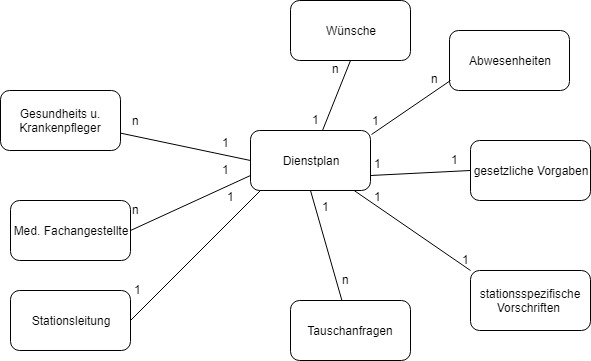
\includegraphics[width=1\textwidth]{Bilder/Domaenenmodell.jpg}
\end{figure}
\section{The Usability Engineering Lifecycle}
In diesem Kapitel wird das zu verwendende Vorgehensmodell bei der Entwicklung von Sister-Shift erläutert und die jeweiligen Schritte für das Projekt geplant. 
Der Usability Engineering Lifecycle ist in drei Phasen unterteilt. Die erste Phase ist die Analyse, danach folgt die Phase der Entwicklung und des Testens und zu Letzt folgt die Phase der Installation. In diesem Projekt wird die Phase der Installation ausgelassen, da es sich im ein Universitätsprojekt in einem simulierten Szenario handelt. Die Möglichkeit das System in einem Krankenhaus zu installieren ist nicht gegeben. Folgend werden die Phasen und die einzelnen Aktivitäten in diesen beschrieben. Nach der Planung der Aktivitäten erhält man einen Usability Project Plan nach dem Muster von Deborah Mayhew. [Deborah J. Mayhew: The Usability Engineering Lifecycle, S. 554]
\subsection{Phase 1: Analyse}
Die Analyse selbst ist wiederum in vier Stufen unterteilt. Die Ergebnisse der Analysephase sind die jeweiligen Usability Goals und ein Styleguide für das System des Projekts.

Stufe 1 – User Profiles

Ein großer Bestandteil dieser Stufe ist es Benutzerprofile zu erstellen. Durch diese soll analysiert werden, wer das System später benutzt und welche Anforderungen die verschiedenen Benutzer jeweils an das System haben. Nach Mayhew gibt es zwei Möglichkeiten die Benutzerprofile zu erstellen. Zum einen gibt es die Möglichkeit von Interviews von Personen aus der Zielgruppe selbst, oder welchen, die die Zielgruppe bestens kennen. Eine andere Möglichkeit bietet das direkte Befragen der Zielgruppe selbst durch das Erstellen und Auswerten von Fragebögen. Mögliche Interviewpartner beim Projekt Sister-Shift sind Gesundheits- und Krankenpfleger oder die Stationsleitung der Notaufnahme. Durch Interviews mit einzelnen Personen kommen allerdings nicht so viele und detaillierte Informationen über die Nutzer zu Tage, wie wenn man mehrere Personen der späteren Nutzergruppe direkt befragt. Diese Befragung erfolgt über das Aushändigen und Auswerten von Fragebögen. Da die Ergebnisse hierbei präziser und detaillierte ausfallen, werden die Benutzerprofile bei der Entwicklung von Sister-Shift über Fragebögen erstellt. [Deborah J. Mayhew: The Usability Engineering Lifecycle, S. 39]
Stufe 2 – Task Analysis

In diesem Schritt werden die Aufgaben der Stationsleitung und Krankenpfleger, die im Zusammenhang mit den Zielen des Systems Sister-Shift stehen, im Detail analysiert. Aus der Analyse können gewissen Anforderungen an das System, welche der Aufgabenerfüllung dienen, herausgestellt werden. Mayhew rät für die perfekte Task-Analyse die zukünftigen Benutzer bei der Arbeit zu begleiten und zu beobachten. Da dies auf der Station der Notaufnahme eines Krankenhauses aus Gründen der Privatsphäre der Patienten und vielen weiteren gesetzlichen Gründen nicht möglich ist, erfolgt die Task-Analysis bei diesem Projekt über Interviews mit Gesundheits- und Krankenpflegern.


Stufe 3 – Platform Capabilities and Constraints
In diesem Schritt werden die Plattformfähigkeiten und Plattformbeschränkungen der von den Nutzern eingesetzten Hardware beschrieben und analysiert. Dafür werden alle wichtigen Aspekte der zu nutzenden Plattform gesammelt und die User Interface Standards für diese untersucht. Das User Interface wird bei Sister-Shift auf den bereits bekannten UI-Standards der Plattform aufbauen und diese auf den Einsatz in der spezifischen Domäne und die jeweiligen Funktionen zuschneiden.

Stufe 4 – General Design Principles
Die vierte Stufe befasst sich mit den generellen Designprinzipien. 
Sind in einer Domäne bestimmte Design Prinzipien bereits vorhanden, so werden diese zunächst untersucht. Dazu werden Styleguides zu Software aus der Domäne, also eines Krankenhauses, betrachtet. Zusätzlich werden übergeordnete Styleguides, wie Plattform-Styleguides benutzt. Um schlussendlich die generellen Designprinzipien zu verfassen, wird auch noch wissenschaftliche Literatur hinzugezogen.
\subsection{Phase 2: Entwicklung und Testen}
 Das weitere Vorgehen in der zweiten Phase des Vorgehensmodells ist nochmals unterteilt. Es folgt eine Beschreibung der drei Level.

Level 1
Nach Erstellung des Styleguides folgt zunächst eine Überarbeitung der einzelnen Artefakte im sogenannten Work Reengineering. Diese Neuausrichtung erfolgt anhand von neu gewonnen Erkenntnissen aus der Task-Flow Analyse und der Benutzerprofile. Folgend werden im Conceptual Model Design die Machbarkeit eines konzeptionellen Modells aufgrund einer Objektanalyse überprüft. Danach werden die erste Designregeln für Ansichten verfasst. Darauf aufbauend werden anschließend verschiedene Wireframes erstellt. Diese Wireframes werden danach zu richtigen Mockups übertragen, und damit in das Design und Layout der Software überführt. Im Regelfall erfolgen hier mehrere Iterationen, um das bestmögliche Ergebnis zu erzielen. [Deborah J. Mayhew: The Usability Engineering Lifecycle, S. 249]

Level 2
In diesem Level werden als erstes die Screen Design Standards erstellt. Diese garantieren der späteren Benutzeroberfläche eine Einheitlichkeit. 

Level 3 
Als letzter Zwischenschritt erfolgt das beschreiben des finalen Detailed User Interface. Nach der Beschreibung erfolgt eine Evaluation des User Interface. Hierbei wird die Methode des Cognitive Walkthrough angewendet. Sofern Fehler erkannt werden, so werden die betroffenen Aspekte in einer Iteration überarbeitet und wiederum getestet.  
\subsection{Phase 3: Installation}
Da eine Installation in einem Krankenhaus und auf Grund der begrenzten Zeit des Projektes nicht möglich ist, wird auf eine finale Installation verzichtet. 
\section{Anforderungen}
Aus der im Konzept durchgeführten Aufgabenmodellierung und Stakeholder-Analyse ergeben sich gewisse Anforderungen, die das System zu erfüllen hat. Diese Anforderungen dienen der ebenfalls im Konzept bestimmten Ziele. Zunächst wird ein Nutzungskontext festgelegt und daraufhin werden die Anforderungen in die Kategorien funktionale, qualitative und organisatorische Anforderungen eingeteilt. 
\subsection{Nutzungskontext}
Der Nutzungskontext basiert auf der Stakeholder-Analyse.
\subsubsection{Stationsleitung}

Die Stationsleitung hat viele verschiedene Aufgaben zu erfüllen. Ein großer Aufgabenbereich ist die Personalverwaltung. Die Stationsleitung erstellt die Dienstpläne für alle Krankenpfleger der jeweiligen Station, kümmert sich bei Personalausfall um Ersatz und kümmert sich um sonstige Angelegenheiten, beispielsweise einen Schichttausch unter Kollegen. In diesem Bereich hat diese einen Berührungspunkt mit dem System.

\subsubsection{Krankenpfleger}
Krankenpfleger sind mit einer der wichtigsten Ressourcen eines Krankenhauses. Diese kümmern sich in erster Linie um Medizinische und sonstige Belange der Patienten. Berührungspunkt mit der Software bietet das Einsehen des eigenen Dienstplans, das melden von Abwesenheit und das Tauschen von Schichten mit Kollegen. 
\subsubsection{restliche Steakholder}
Die übrigen Stakeholder, welche bei der Stakeholder-Analyse ermittelt wurden, haben keine direkten Berührungspunkte mit dem System Sister-Shift. Demnach werden diese im Nutzungskontext nicht berücksichtigt. 
\subsection{Anforderungsanalyse}
Folgend werden die Anforderungen an das System beschrieben und in die jeweiligen Kategorien aufgeteilt. Die funktionalen Anforderungen sind dabei die Anforderungen, die das System erfüllen muss. Qualitative Anforderungen beschreiben die Eigenschaften des Systems. Die organisatorischen Anforderungen bezeichnen die Anforderungen, die das System erfüllen muss, damit der spätere Benutzer dieses nutzen kann.
\subsubsection{Funktionale Anforderungen}
[FA01] Das System muss Gesundheits- und Krankenpflegern die Möglichkeit bieten Ihren aktuellen Dienstplan einzusehen\\\\
[FA02] Das System muss bei der automatischen Erstellung der Dienstpläne alle gesetzlichen und Krankenhaus spezifischen Gesetze und Regelungen beachten und einhalten\\\\
[FA03] Das System sollte den Gesundheits- und Krankenpflegern die Möglichkeit bieten persönliche Wünsche zur Einsatzplanung vor der Dienstplanerstellung an dieses mitzuteilen\\\\
[FA04] Das System muss fähig sein, einen umfassenden Dienstplan für jeden Tag und mit Berücksichtigung jeglicher Schicht, und (soweit wie möglich) der individuellen Wünsche der Mitarbeiter automatisch zu generieren\\\\
[FA05] Das System muss den Mitarbeitern die Möglichkeit bieten, eine Abwesenheit zu hinterlegen\\\\
[FA06] Sobald eine Abwesenheitsmeldung vorliegt, muss das System fähig sein, automatisch einen Ersatz zu organisieren und einzuteilen\\\\
[FA07] Ist ein Ersatz für einen Personalausfall gefunden und eingeteilt, so muss das System die Dienstpläne der betroffenen Mitarbeiter automatisch anpassen, und die betreffenden Personen + die Stationsleitung über die Änderungen benachrichtigen\\\\
[FA08] Falls kein Mitarbeiter aus dem eigenen Krankenhaus als Ersatz bei Personalausfall einspringen kann, soll das System bei externen Firmen Personal für den betroffenen Zeitraum anfragen\\\\
[FA09] Das System muss den Gesundheits- und Krankenpflegern nachdem ein Dienstplan generiert wurde die Möglichkeit bieten, untereinander mit Hilfe des Systems Schichten zu tauschen\\\\
[FA10] Falls ein Schichten-Tausch angestrebt wird, darf das System nur Tausche zulassen, welche die gesetzlichen und Krankenhaus spezifischen Gesetze und Vorgaben nach dem Vollziehen dieser, immer noch erfüllen\\\\
[FA11] Das System muss der Stationsleitung die Möglichkeit bieten, Aspekte und Kenngrößen zu dem zu erstellenden Dienstplan festzulegen\\\\
\subsubsection{Qualitative Anforderungen}
[QA01] Das System muss dem Nutzer den Dienstplan und sonstige Informationen schnell und verständlich bereitstellen. Es muss leicht verständlich und gut bedienbar sein, damit auch ältere Gesundheits- und Krankenpfleger schnell den Gebrauch dieses lernen\\\\
[QA02] Das System eine hohe Systemstabilität aufweisen. Es soll also sehr wartungsfreundlich sein\\\\
[QA03] Das System soll zuverlässig sein. Die Dienste sollen immer zur Verfügung stehen\\\\
\subsubsection{Organisatorische Anforderungen}
[OA01] Das System soll über verschiedene Endgeräte genutzt werden können. Dies beinhaltet sowohl den Desktop vom Computer am Arbeitsplatz, als auch diverse mobile Endgeräte\\\\
[OA02] Das System muss jeden Mitarbeiter auffordern eine valide Kontaktmöglichkeit zu hinterlegen\\\\
[OA03] Die Daten der einzelnen Mitarbeiter und deren Dienstplänen müssen so geschützt sein, dass nicht gegen die\\\\ Datenschutzverordnung verstoßen wird
[OA04] Die Einführung des Systems sollte so kostengünstig wie möglich sein\\\\
\subsection{Priorisierung der ermittelten Anforderungen}
Die ermittelten Anforderungen sind in Bezug auf die Zielerreichung unterschiedlich zu gewichten. Folgend ist eine Tabelle mit einer Priorisierung der Anforderungen zu sehen. Die Priorisierung umfasst die Zahlen 1-5, wobei 5 die höchste Priorität darstellt.
\begin{figure}[H]
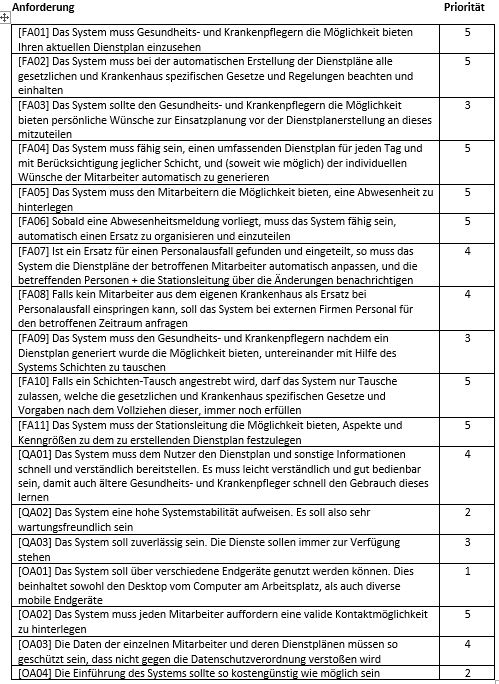
\includegraphics[width=1\textwidth]{Bilder/Tanforderungen.png}
\caption{Anforderungspriorisierung}
\end{figure}
\subsubsection{Fazit}
Die Priorisierung zeigt, dass der Schwerpunkt der wichtigen Anforderungen auf den funktionalen Anforderungen liegt. Die Benutzer des Systems sollen im Stande sein, die Hauptfunktionalitäten von Sister-Shift zu nutzen. Diese unterstützen vor allem die Stationsleitung bei der Personalplanung, erleichtern aber auch die Kommunikation zwischen Krankenpfleger und Stationsleitung. Zusätzlich werden auch die Krankenpfleger durch weniger Zeit- und Kommunikationsaufwand entlastet.
\section{User Profiles}
In diesem Kapitel werden User Profile der zukünftigen Benutzer des Systems erstellt und aus einer Umfrage [vgl. Anhang Umfrage] von Pflegepersonal der Notaufnahme Leverkusen Schlebusch Rückschlüsse auf bestimmte Anforderungen gegenüber dem System ermittelt. Dabei können die analysierten Anforderungen sowohl Technischer, Inhaltlicher und Visueller Natur sein. Die Ergebnisse ergänzen die bereits analysierten Anforderungen. Das Schema der Analyse wurde anhand von Mayhew erarbeitet. [vgl. Mayhew Chapter 2]

\subsection{Stationsleitung}
Die Stationsleitung übernimmt viele verschiedene Aufgaben. Bestandteil der wesentlichen Aufgaben ist die Personalplanung. Diese umfasst das Erstellen der Dienstpläne. In Zusammenhang damit, kümmert die Stationsleitung sich natürlich auch um die Organisation bei Personalausfall und sonstigen personellen Anliegen. 

\subsubsection{Eigenschaften}
Die Stationsleitung arbeitet überwiegend im Büro der jeweiligen Station. In die Erstellung eines Dienstplans fließt viel Zeit, da unterschiedliche Mitarbeiter viele individuelle Wünsche haben. Zusätzlich müssen große Mengen an Informationen bezüglich Arbeitsschutzgesetz und Jugendschutz vorhanden sein. Dazu kommen noch die Stationsabhängigen Besonderheiten, die eventuell eingehalten werden müssen. Die Stationsleitung nutzt aktuell Excel zur Erstellung der Dienstpläne. Sofern das neue System gut zu benutzen, zuverlässig und verständlich ist, ist die Stationsleitung aufgeschlossen, neue Methoden und Systeme anzunehmen.  

\subsubsection{Anforderungen}
Die Stationsleitung legt Wert auf den Ease of Use und den Ease of Learning, da sie bisher keine Erfahrungen mit Personalplanungssoftware hat, und sie auf jeden Fall ein besseres Ergebnis in der Personalplanung erreichen möchte. Der Einsatz von ICONS oder Grafiken unterstützt diesen Anspruch. Als Zusatz sollte die Leitung Verwaltungs-Optionen bereitgestellt bekommen um das Personal ausreichend einzuplanen.
\subsection{Krankenpfleger}
Die Krankenpfleger haben die Hauptaufgabe, die Patienten für die Behandlung durch die Ärzte vorzubereiten. Anschließend unterstützen sie die Ärzte bei der weiteren Versorgung der Patienten. Die Behandlung ist in einen internistischen und einen chirurgischen Bereich zu unterteilen. Internistisch muss den Patienten beispielsweise eine Blutprobe entnommen werden, ein EKG geschrieben werden oder Medikamente verabreicht werden. Im chirurgischen Bereich müssen Patienten mit Verletzungen versorgt werden, das beinhaltet z.B. das gipsen von Brüchen oder das reinigen und nähen von Wunden. Nicht zu unterschätzen ist die Reanimation eines Patienten, die höchste Priorität hat, und meist körperlich sehr anstrengend ist. Falls ein Patient mit einem Rettungswagen eingeliefert wird, ist es die Aufgabe der Krankenpfleger diesen Patienten im Computer System aufzunehmen und die Behandlung dort zu dokumentieren. Falls der Patient selbständig in die Notaufnahme gekommen ist, muss nur die Behandlung dokumentiert werden. Aus Organisatorischer Sicht müssen sich die Krankenpfleger so früh wie möglich abwesend melden, falls sie verhindert sind, und auf Ersatzanfragen Antworten, falls Sie diese erhalten. Falls Krankenpfleger Schichten untereinander Tauschen geschieht dies auf einem privaten Kanal.
\subsubsection{Eigenschaften}
Die Krankenpfleger haben bereits längere Erfahrungen mit verschiedener Software, wie z.B. KIS der Nexus AG, die sie täglich am Arbeitsplatz nutzen. Sie fühlen Sich durch den Computer in ihrer Arbeit unterstützt, und stehen diesem auch weitestgehend positiv gegenüber. Die Auffassung für Änderungen am Arbeitsplatz ist ebenso positiv. Jedoch ist die Bereitschaft für neue Software nur gegeben, falls diese einen deutlich unterstützenden Beitrag im Arbeitsalltag leistet. Eine Weitsichtigkeit ist nur geringfügig vorhanden. Der Bildungsgrad ist durchwachsen von Berufsschulabschlüssen über Realschulabschlüssen und dem Abitur.
\subsubsection{Anforderungen}
Die Krankenpfleger umfassen das gesamte Arbeitsspektrum von der Aufnahme eines Patienten bis zur Entlassung. Zwar haben die Pfleger Erfahrungen mit Software, jedoch keiner, der der Organisation der Personalplanung dient. KIS beispielsweise ist eine Software für die Dokumentation von Patienten Prozessen. Dies Bedeutet, das Sister Shift als Software etwas komplett Neues für die Pfleger ist, wodurch ein besonders einfaches und leicht zu verstehendes Design nötig sein wird, um die Lernkurve möglichst niedrig zu halten und den Pflegern keine zusätzliche Belastung zuzumuten. 
Infolgedessen bietet es sich an, besonders gängige ICONS und Grafiken zur Vereinfachung des Verständnisses zu verwenden.

\subsection{Medizinische Fachangestellte}
Die Medizinischen Fachangestellten sind primär für die Aufnahme neuer Patienten am Empfang zuständig, Sie entscheiden wie gravierend ein Notfall ist, und legen die Reihenfolge der Patienten die als nächstes behandelt werden fest. Außerdem organisieren sie den Patiententransport auf andere Stationen, dies beinhaltet die Anfrage an die jeweilige Verlegungsstation und den Auftrag an den Patiententransport für die Abholung des Patienten. 
\subsubsection{Eigenschaften}
Die Medizinischen Fachangestellten sehen den Computer, anders als die Krankenpfleger, als ihr primäres Arbeitsutensil an. Sie fühlen sich durch den Computer effizienter und mögen die Arbeit mit ihm weitestgehend. Neuer Software stehen Sie erstmal kritisch gegenüber, aber sie sind lernbereit sobald sie eine Unterstützung durch das System sehen. Die Erfahrungen mit Computer Software sind hier noch stärker als bei den Krankenpflegern aber wieder dominiert hier die Software KIS von der Nexus AG. Eine Kurzsichtigkeit ist verbreitet sowie der mittlere Bildungsgrad.
\subsubsection{Anforderungen}
Die Medizinischen Fachangestellten, haben wie die Krankenpfleger keine Erfahrungen mit einer Personalplanungssoftware, woraus sich dieselben Anforderungen bezüglich der Übersichtlichkeit und Einfachheit ergeben.
\subsection{Zusammenfassung}
Die Folgende Tabelle fast die wichtigen Anforderungen bezüglich der Benutzerfreundlichkeit nach Benutzerkategorien zusammen.\\\\
Die Anforderungen sind:\\\\
Ease of Learning – Wie schnell und einfach kann ein Benutzer die neue Computersoftware erlernen?\\\\
Ease of Use – Wie schnell und effizient kann ein Benutzer eine Aufgabe mit der Computersoftware bearbeiten?\\\\
Simplicity - Wird ein hoher Grad an Einfachheit benötigt, um Aufgaben zu bewältigen?\\\\
Visuals/ICONS – Sollten Informationen mithilfe von Icons oder Grafiken visualisiert werden?\\\\
Minimize typing – Wie stark sind die Tipp Fähigkeiten an der Tastatur? Ist ein Point and select einem remember and Type bevor Zuzügen?\\\\
Color vision deficit- Wie verbreitet ist Farbenblindheit unter den Benutzern?\\\\
Other vision deficit – Wie verbreitet sind andere Sehschwächen unter den Benutzern?\\\\
\begin{figure}[H]
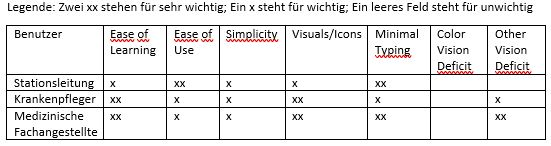
\includegraphics[width=1\textwidth]{Bilder/tabelleAuswert.jpg}
\caption{Auswertung}
\end{figure}
\section{Task Analyse}
Im Folgenden werden die für unser System wichtigen Aufgaben inklusive der Arbeitsschritte beschrieben. Die Analyse erfolgte in zusammen Arbeit mit einer Krankenpflegerin der Ambulanz des Klinikums Leverkusen. Zunächst wird die Aufgabe genannt, dann werden die Akteure genannt, dann der Ablauf der Aufgabe, dann die Zeitlichen Rahmenbedingungen und anschließend die Anforderungen an das Benutzer-Interface. Die Medizinischen Fachangestellten wurde im Folgenden nicht genannt, da sie die exakt selben schritte wie die Krankenpfleger bezüglich folgender Tasks übernehmen würden.
\subsection{Task Einreichen einer Krank-/Abwesenheitsmeldung}
Actor\\\\
Krankenpfleger; Stationsleitung\\\\
Flow\\\\
Krankenpfleger\\\\
Ein Mitarbeiter meldet sich in der Notaufnahme bei einem seiner Kollegen krank bzw. abwesend.\\\\
1.	Der Krankenpfleger, der das Telefonat angenommen hat, notiert sich schriftlich die Informationen des sich krankmeldenden Kollegen auf einem Zettel.\\\\
2.	Diese Notiz übermittelt der Krankenpfleger nun an die Stationsleitung, ist diese nicht im Haus, wird die Notiz an einen Kollegen der nächsten Schicht übergeben. Dies wiederholt sich so oft bis die Notiz die Stationsleitung erreicht, die sich dann um die nächsten Schritte kümmern kann.\\\\
Zusatz: Ist die Stationsleitung oder deren Vertretung aus Gründen wie Krankheit länger nicht zu erreichen, werden die Folgenden schritte von einer regulären Pflegekraft übernommen.\\\\
Stationsleitung\\\\
1.	Die Stationsleitung erreicht die Information, dass es einen Ausfall in einer zukünftigen Schicht gibt. Sie trägt dies Im Dienstplan der Abwesenden Person ein. \\\\
2.	Sie ermittelt welche Mitarbeiter an diesem Tag frei haben.\\\\
3.	Kandidaten die 11 bzw. 10 Stunden Arbeitsunterbrechung bei Übernahme nicht erreichen schließt sie zusätzlich aus.\\\\
4.	Bei den übrig gebliebenen Kandidaten fragt sie eine Übernahme an.\\\\
5.	Sobald sich der erste mit einer Zusage meldet trägt Sie dies in den Dienstplan des übernehmenden Mitarbeiters ein. Und bestätigt ihm die Übernahme.\\\\
Zusatz: Ist eine Person mehr als einen Tag krank bzw. abwesend, wiederholen sich Schritt 2 bis 5 für jeden Tag der Abwesenheit. Kommt es zu dem Fall, das sich kein interner Ersatz findet, wird Ersatz über eine Zeitarbeitsfirma organisiert.\\\\
Task Closure\\\\
Die Dauer einer Instanz dieses Szenarios, ist von der Anwesenheit der Stationsleitung, der Meldung eines Ersatzes und dem Zeitpunkt der Abwesenheit abhängig. Ist die Stationsleitung anwesend erreicht Sie die Nachricht innerhalb der ersten zehn Minuten nach Eingang. Ist sie es nicht und ist die Abwesenheit noch ausreichend weit entfernt kann es zwischen und 8 und 16 Stunden dauern, das die Stationsleitung oder deren Vertretung die Nachricht über den Ausfall erhält. Die Zeitspannen bis sich ein Ersatz meldet kann ebenso sehr stark variieren. Aufgrund dieser vielen Variablen kann man keine genaue Angabe machen wie lange dieses Szenario durchschnittlich andauert. Wenn alle Personen anwesend sind und sich ein Ersatz schnell findet, kann dies in unter einer Stunde geschehen, ansonsten kann dies aber auch mehrere Tage andauern.\\\\
User-Interface Requirements 
Den Krankenpflegern muss es ermöglicht werden sich über das Interface abwesend zu melden, zu dem haben Sie den Anspruch andere Abwesenheiten einzusehen, um einen überblick darüber zu haben mit wem sie gemeinsam Dienst haben.\\\\
Die Stationsleitung muss einen überblick darüber haben wer sich wann und für wann abwesend gemeldet hat und für wen bereits Ersatz gefunden wurde, für wen bereits Ersatz angefragt wurde und für wen noch nicht. Außerdem ist für sie der Grund der Abwesenheit wichtig. Bezüglich der Ersatzfindung muss es ihr möglich sein, die für den Ersatz bereitstehenden Mitarbeiter einzusehen und diese ggf. zu selektieren, bevor sie diese Anfragt.\\\\
\subsection{Task Verfassen des Dienstplans}
Actor\\\\
Krankenpfleger; Stationsleitung \\\\
Flow\\\\
Krankenpfleger \\\\
1.Der Krankenpfleger äußert über ein in der Station ausgelegtes Buch, seine Wünsche bezüglich der Dienstplangestaltung für den übernächsten Monat.\\\\
Stationsleitung\\\\
1.Nach Ablauf der Frist für die Wunschäußerung, nimmt die Leitung das Wunschbuch an sich.\\\\
2.Sie beginnt die Wünsche zu analysieren und notiert sich potenzielle Konflikte.\\\\
3.Sie trägt nicht konfliktäre Wünsche in den Dienstplan ein.\\\\
4.Interpersonelle Konflikte werden von der Stationsleitung versucht zu lösen und daraufhin in den Dienstplan eingetragen.\\\\
5.Die Leitung notiert alle Wünsche die nicht berücksichtigt werden können.\\\\
6.Die Stationsleitung beginnt das Personal auf die restlichen Schichten des Dienstplans zu verteilen. Dabei achtet Sie darauf, dass die Verteilung fair verläuft, dies bedeutet das eine ausgeglichene Verteilung der Schichtenarten, der Wochenendschichten und der freien Tage eingehalten wird.\\\\
7.Sie überprüft ob der Dienstplan gesetzliche aber auch Krankenhaus spezifische Rahmenbedingungen einhält, falls nicht, passt sie diesen an.\\\\
8.Die Stationsleitung informiert die Mitarbeiter deren Wünsche nicht erfüllt werden konnten, falls dies nicht schon unter Punkt 4 geschehen ist.\\\\
9.Sie hängt den Dienstplan für die Krankenpfleger aus.\\\\

Task Closure
Die Dauer des Verfassens des Dienstplanes hängt von der Anzahl der Wünsche und die damit zusammenhängenden Konflikte ab. Dieser Vorgang dauert zwischen 6 und 10 Stunden.\\\\
User-Interface Requirements
Den Krankenpfleger muss es ermöglicht werden ihre Wünsche über das Interface zu äußern.\\\\
Der Stationsleitung muss es möglich sein diese Wünsche einzusehen. Es sollte hervorgehoben werden welche Wünsche Konfliktär sind, welche erfüllbar oder nicht erfüllbar sind. Nach der Erstellung des Dienstplans durch das System unter der Einhaltung aller Rahmenbedingungen, sollte eine Liste, der nicht erfüllten Wünsche, der Stationsleitung bereitstehen, um auf Rückfragen des Personals antworten zu können. Zu dem soll das Personal über nicht erfüllte Wünsche informiert werden.
Der Dienstplan soll daraufhin von der Stationsleitung für das Personal veröffentlich werden können.\\\\
\subsection{Task Tausch einer Schicht}
Actor\\\\
Krankenpfleger; Stationsleitung \\\\
Flow \\\\
Krankenpfleger\\\\
1.Private Absprache mit einem Kollegen über einen Schichtentausch.\\\\
2.Der Pfleger übermittelt der Stationsleitung den Wunsch des Tauschs.\\\\
Stationsleitung\\\\
1.Die Stationsleitung nimmt den Wunsch entgegen.\\\\
2.Sie prüft ob der Tausch gesetzlich aber auch Krankenhaus spezifisch vollzogen werden darf.\\\\
3.Sie ändert den Dienstplan der beiden tauschenden Pfleger, und holt sich die Bestätigung bei beiden ein.\\\\
Task Closure\\\\
Nach Absprache der Kollegen, kann je nach Anwesenheit der Stationsleitung oder deren Vertretung der Tausch der Schicht zwischen 15 Minuten und 16 Stunden dauern.\\\\
User-Interface Requirements\\\\
Den Krankenpflegern soll es ermöglicht werden ihre Schichtauschanfrage über das System zu äußern. Das System soll darauf autonom prüfen ob dieser möglich wäre, falls dies möglich ist soll dieser Tausch vollzogen werden. Daraufhin sollen Krankenpfleger und Stationsleitung über dieses Ereignis informiert werden. Stellt sich heraus das ein Tausch zwischen den Krankenpflegern nicht möglich ist, sollen diese darüber informiert werden und potentielle andere Tauschpartner vorgeschlagen bekommen.
\subsection{Fazit}
Mit Hilfe dieser Analyse konnten, die vom System zu übernehmenden Arbeitsschritten bezüglich dieser Tasks identifiziert werden. Das System wird eine viel transparentere Personalplanung für alle Mitarbeiter ermögliche. Zu dem wird die Kommunikation vereinfacht und wichtige Informationen wie die Wünsche oder der Dienstplan visualisiert.
\section{Usability Goals}
Folgend werden die Ergebnisse aus der Benutzermodellierung und der Task-Analyse ausgewertet und die Usability Goals, welche für das Design des Systems relevant sind ermittelt. 
\subsection{Qualitative Usability Goals}
Die qualitativen Ziele an das User-Interface stellen allgemeine Ziele an das Interface dar, auch wenn diese nicht messbar sind. [Deborah J. Mayhew: The Usability Engineering Lifecycle, S.126] 
Als Grundlage zur Ermittlung der genannten Ziele, dient die Benutzermodellierung und die daraus entstandenen User-Profiles. Die Task-Analyse dient als Zusatz.
\begin{figure}[H]
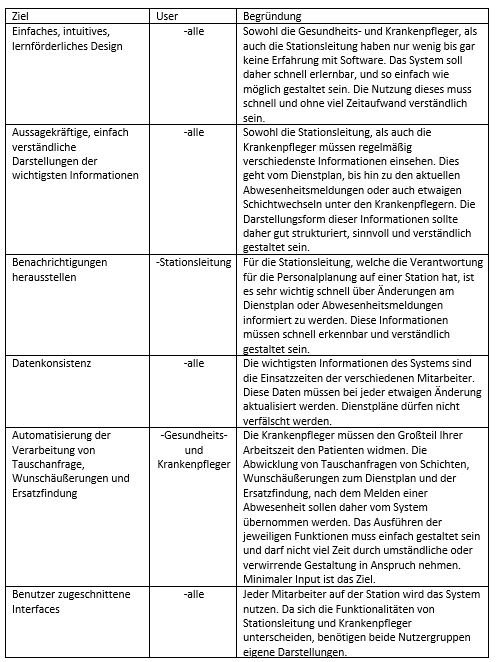
\includegraphics[width=1\textwidth]{Bilder/qualiUser.jpg}
\caption{Qualitative Usability Goals }
\end{figure}
\subsection{Quantitative Goals}
\subsubsection{Dienstplanerstellung / -abfrage}
Die Erstellung und vor allem das Abrufen des Dienstplanes ist eine der Hauptfunktionen. Die Stationsleitung erstellt mit Hilfe des Systems Dienstpläne, welche alle domänenspezifischen und gesetzlichen Bedingungen einhalten. Das System soll außerdem Mitarbeiterwünsche mit einpflegen. Anschließend werden diese Dienstpläne von allen Benutzern des Systems abgerufen. Die Priorität dieses Ziels ist somit sehr hoch.
\begin{figure}[H]
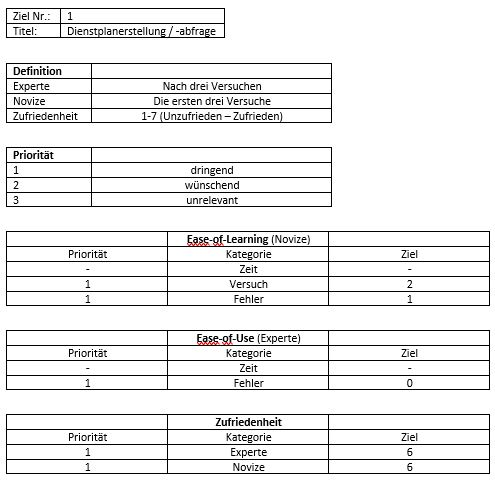
\includegraphics[width=1\textwidth]{Bilder/dienstplanAbfrage.jpg}
\end{figure}
\subsubsection{Melden von Abwesenheit}
Das Melden einer Abwesenheit ist für die Gesundheits- und Krankenpfleger eine wichtige Funktion, da hier eine Menge Arbeit auf das System umgeleitet werden kann. Das Finden eines Ersatzes soll vom System übernommen werden. Demnach ist das Ease-of-Use hier besonders hoch priorisiert, weil die Gesundheits- und Krankenpfleger als hoch motivierte User gelten um diese Funktion zu nutzen.
\begin{figure}[H]
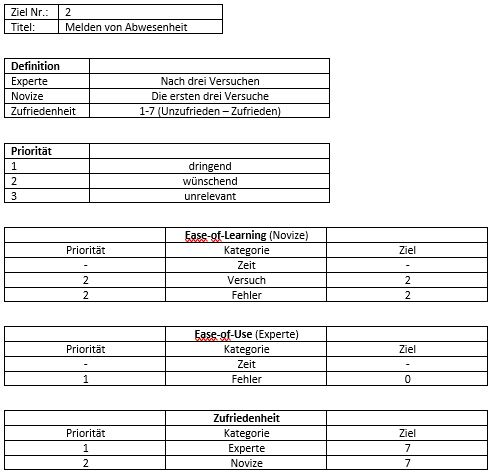
\includegraphics[width=1\textwidth]{Bilder/meldenAbwesen.jpg}
\end{figure}
\subsubsection{Schichttausch}
Diese Funktion wird ebenfalls mit einem hohen Ease-of-Use priorisiert, da die Gesundheits- und Krankenpfleger mit dieser unabhängig von der Stationsleitung Ihren Dienstplan, sofern möglich, individualisieren können. Mit dieser Funktion können Kollegen Schichten untereinander tauschen, sofern die automatische Prüfung des Systems auf Einhaltung der domänenspezifischen und gesetzlichen Bedingungen dies zulässt. Somit sind diese auch hier wieder motivierte User der Funktion.
\begin{figure}[H]
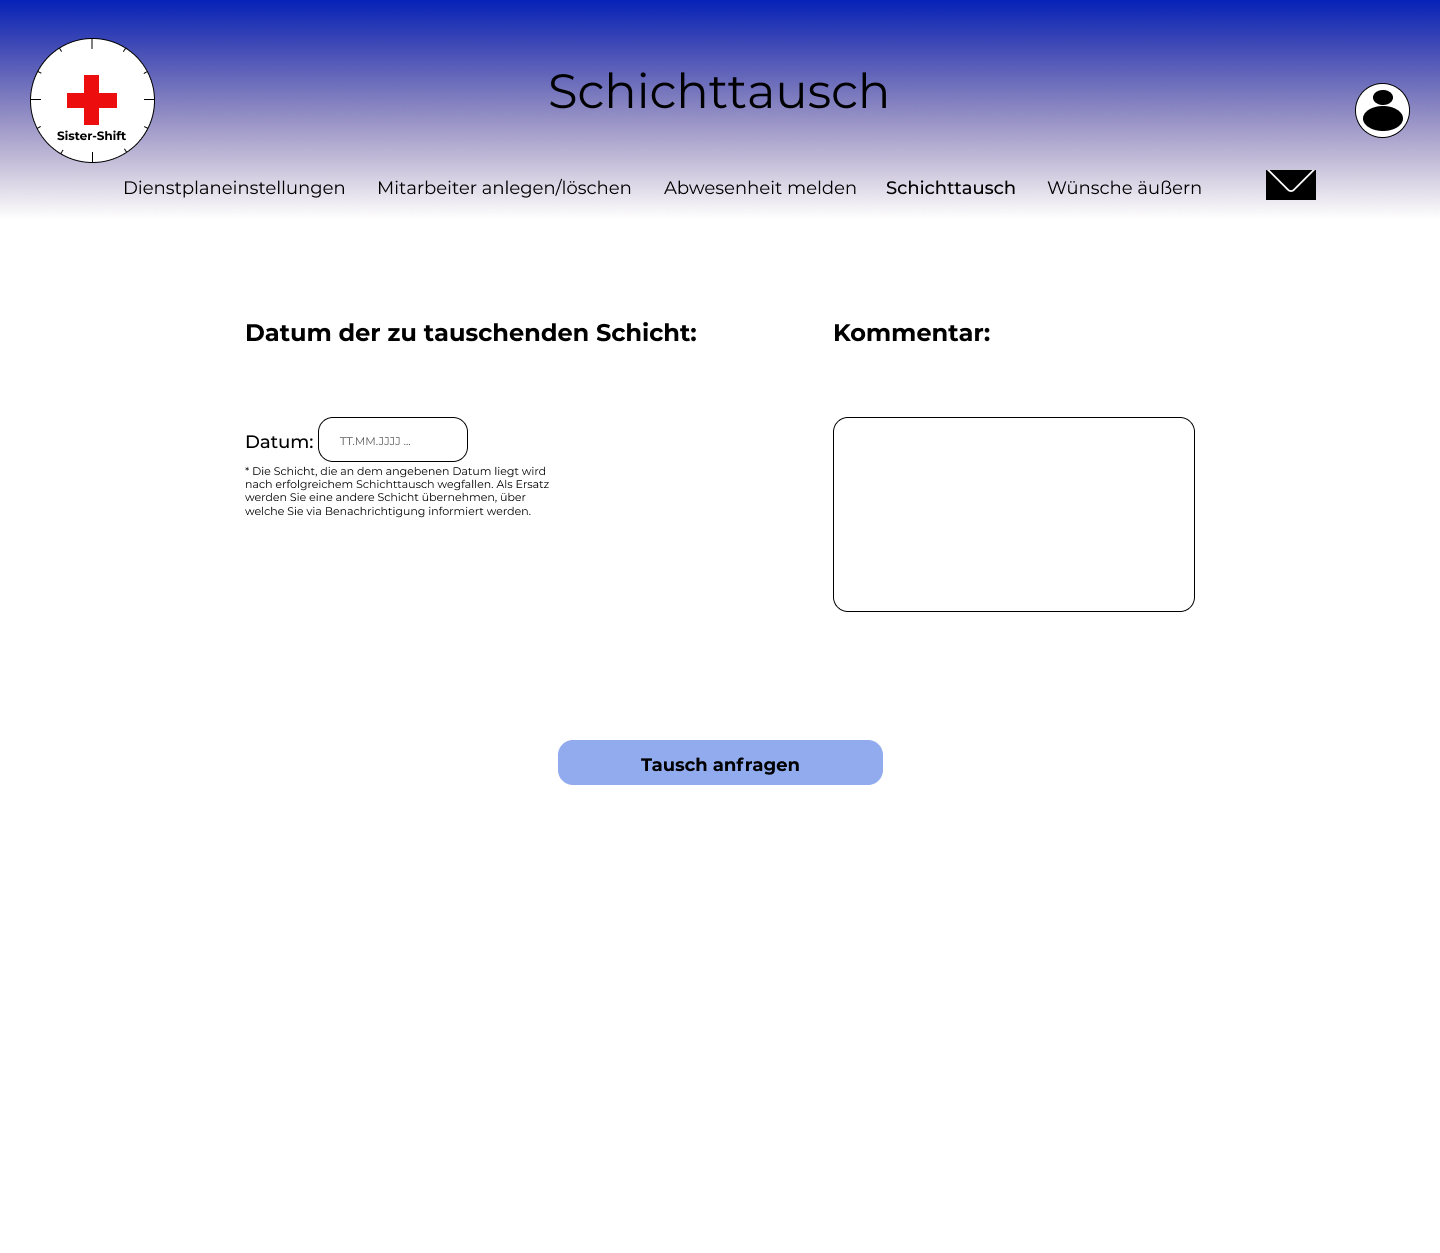
\includegraphics[width=1\textwidth]{Bilder/Schichttausch.jpg}
\end{figure}
\subsubsection{Eintragen von Wünschen zur Schichtplanung}
Die Mitarbeiter sollen die Möglichkeit haben Wünsche zur Dienstplanung an das System mitzuteilen, welche dann von diesem bei der Dienstplanerstellung berücksichtigt werden sollen. Auch hier ist eine hoher Ease-of-Use zu verzeichnen und dementsprechend zu priorisieren. Da der Dienstplan aber auch so erstellt wird, ist die Priorität etwas geringer.
\begin{figure}[H]
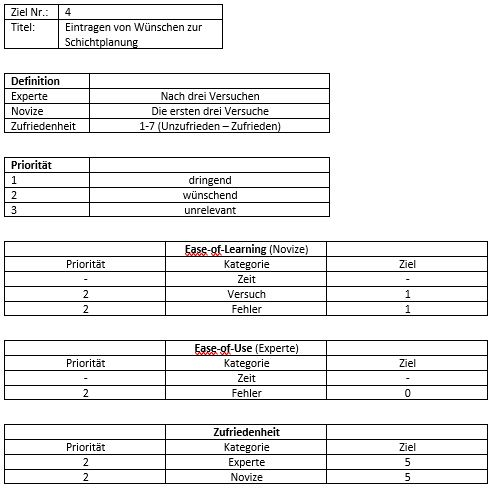
\includegraphics[width=1\textwidth]{Bilder/wuensche.jpg}
\end{figure}
\section{Platform Capabilities and Constraints}
\subsection{Anwendung für Gesundheits- und Krankenpfleger Personal und die Stationsleitung}
Die Anwendung wird sowohl für die Gesundheits- und Krankenpfleger, als auch die Stationsleitung für Desktop-Computer und/oder Laptops konzipiert. Durch die Festlegung auf diese Plattform, ergeben sich spezielle Rahmenbedingungen. Zusätzliche Bedingungen ergeben sich durch die Umsetzung als Web-Anwendung und der damit verbundenen Nutzung verschiedener Hard- und Softwareplattformen.
\subsection{Bildschirmgröße}
Eine spezielle Bildschirmgröße ist durch die Umsetzung als Web-Anwendung mit einem responsiven Design nicht zu beachten. In einer Notaufnahme eines Krankenhauses sind die Computer, welche für die Gesundheits- und Krankenpfleger zur Verfügung stehen, mit ausreichend großen Monitoren 
versehen.
\subsection{Browser}
Um die Anwendung Sister-Shift nutzen zu können, wird ein Browser benötigt. Dieser sollte HTML5 fähig sein. Vorinstallierte Browserplugins sind für die Nutzung der Anwendung nicht erforderlich.
\subsection{Anbindung}
Die Anwendung erfordert nur eine Schmalbandverbindung zum Internet, da keine Videos oder Livestreams ausgetauscht werden. Demnach wird keine Breitbandverbindung vorausgesetzt. Da der Dienstplan übersichtlich und in passender Form dargestellt werden muss, wird auf eine “Nur-Text-Version” der Anwendung verzichtet.
\subsection{Ein- und Ausgabegeräte}
Die primären Eingabegeräte sind Maus und Tastatur. Etwaige Touchscreens gelten nicht als primäre Eingabequelle. Als primäres Ausgabegerät dient der jeweilige Bildschirm oder Laptop. Weitere Ein- oder Ausgabegeräte zur Nutzung von Sister-Shift sind nicht geplant.
\section{General Design Principles}
Folgend werden die generellen Design Prinzipien untersucht. Dies ist wichtig, um die Benutzbarkeit des Systems für den Nutzer zu gewährleisten und um die Anforderungsanalyse des Usability Engineering Lifecycles abzuschließen. Nach Mayhew ist diese Untersuchung in zwei Schritte zu gliedern. 
Im ersten Schritt erfolgt die Untersuchung von High Level-Styleguides. Hierbei werden übergeordnete Style-Guides im Unternehmen selbst angeschaut. Diese vermitteln ein gemeinsames Aussehen und Gefühl. Zusätzlich wird durch diese ein einheitliches Corporate Image für die Organisation selbst sichergestellt.
Im zweiten Schritt erfolgt die Hinzunahme anderer Quellen. Dazu zählen Fachzeitschriften, Bücher oder sonstige Erzeugnisse, welche sich mit General Design Principles beschäftigen. Die anderen Quellen sollten nicht mit den High Level-Styleguides in Beziehung stehen. Mayhew beschreibt unter diesem Punkt benutzerspezifische Prinzipien, welche beachtet werden müssen. [Deborah J. Mayhew: The Usability Engineering Lifecycle, S.163]

Der Aufbau der Applikation des Systems Sister-Shift wird sich an einem Framework orientieren, da es keine übergeordneten Styleguides und auch keine Basis-Styleguide in der Notaufnahme eines Krankenhauses gibt. Das zu benutzende Framework wird Semantic UI sein, da es laut Mayhew keine User-Interface-Standards für das Web gibt. [Deborah J. Mayhew: The Usability Engineering Lifecycle, S.166]
\subsection{Abwägung des zu verwendenden Frameworks}
Wie o.g. handelt es sich bei Semantic UI um ein User-Interface Framework. Mit diesem es einfach zeitgemäße und responsive Webseiten und Webanwendungen zu erstellen. Semantic UI hebt sich durch eine gute Strukturierung und eine gute Lernförderlichkeit von anderen ähnlichen Frameworks ab. Ein großer Vorteil gegenüber z.B. Bootstrap und wichtig für den begrenzten Projektzeitraum, ist das Vorhandensein von verschiedenen UI- Elementen, wie Dropdownmenüs und eine einfache Klassenbenennung.
\subsection{Andere Quellen}
Mayhew gibt hier durch eine List von Fachliteratur Hilfestellung bei der Findung der geeigneten Quelle. [Deborah J. Mayhew: The Usability Engineering Lifecycle, S.163]
\section{Styleguide}
\subsection{Farbpalette}
Eine der wichtigsten Faktoren im Design sind die verwendeten Primär- und Sekundärfarben. Da das System schnell erlernbar und einfach zu verwenden sein soll, müssen die gewählten Farben dies wiederspiegeln. Die Farben müssen präzise festgelegt sein, um einen einheitlichen Look und eine Wiedererkennbarkeit zu gewährleisten. Als Primärfarbe ist Blau und als Sekundärfarbe ist Grün festgelegt. Die Akzentfarbe ist dabei blau. Die Farbe steht für Leichtigkeit und Schwerelosigkeit. Diese Attribute sollen die einfache Bedienung und das schnelle Erlernen des Systems repräsentieren. Die Sekundärfarbe Grün steht für Hoffnung und hat eine entspannende Wirkung. Sie ist somit positiv geprägt. Grün dient, in geringerem Maße eingesetzt, dem Hervorheben und Ergänzung der Primärfarbe Blau. Bei Texten kommt schwarz zum Einsatz. Um weiter die Übersichtlichkeit und Einfachheit zu unterstützen, ist die Hintergrundfarbe reines weiß.
\subsection{Farbfond}
Für Farbflächen gibt es einen Farbfond. Dieser wird bei großen Flächen und neben den Akzentfarben eingesetzt. Der definierte Blauverlauf ist auch auf größeren Flächen angenehm für den Betrachter. Er vermittelt eine edle Optik und eine gewisse Leichtigkeit. Zusätzlich vermittelt der gewählte Fond eine abwechslungsreiche Dynamik. Er ist wie folgt definiert: 
\begin{figure}[H]
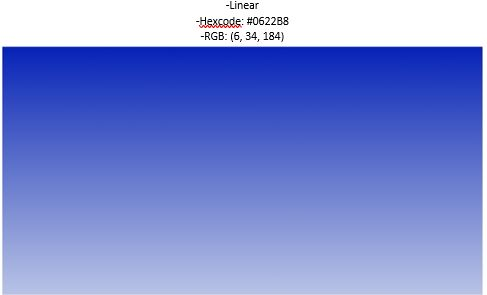
\includegraphics[width=1\textwidth]{Bilder/farbfont.jpg}
\caption{Farbfond}
\end{figure}
\subsection{Hintergrundfarben}
\begin{figure}[H]
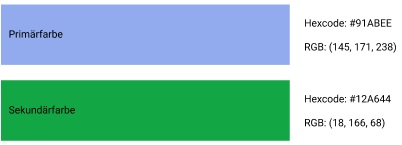
\includegraphics[width=1\textwidth]{Bilder/Hintergrundfarben.jpg}
\caption{Hintergrundfarben}
\end{figure}
\subsection{Textfarbe}
\begin{figure}[H]
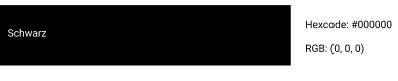
\includegraphics[width=1\textwidth]{Bilder/Textfarben.jpg}
\caption{Textfarbe}
\end{figure}
\subsection{Typographie}
Der im System verwendetet Schriftart ist Montserrat. Diese bietet verschiedene Schnitte, welche von Extra Light bis Bold reichen, und ist damit umfangreich ausgestattet.
\begin{figure}[H]

\includegraphics[width=1\textwidth]{Bilder/Typographie.jpg}
\caption{Typographie}
\end{figure}
\subsection{Logo}
Das Logo der Anwendung Sister-Shift wurde extra für diese entworfen. 
\begin{figure}[H]
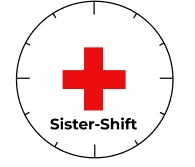
\includegraphics[width=1\textwidth]{Bilder/Logo.jpg}
\caption{Logo}
\end{figure}
\subsection{Webfont}
Die Schriftart Montserrat ist unter Google Fonts gelistet und zu finden. Demnach kann jede Plattform diese als Webfont lizensieren und einsetzen. Somit wird plattformübergreifend das gleiche Schriftbild gewährleistet.
\subsection{Schriftgröße}
Die Schriftgröße von Montserrat ist in Fließtexten auf 11 mit einem angemessenen Zeilenabstand zu setzen. Überschriften sind von der Schriftgröße her frei skalierbar. Überschriften von Fließtexten sollten jedoch im Verhältnis zur oben genannten Schriftgrößte des Textes sein. Der Zeilenabstand ist gering zu halten, sodass Headline und Fließtext ein kompaktes Gesamtbild ergeben. Es sollte jedoch drauf geachtet werden, dass die Zeilen immer noch unterscheidbar sind. Die Schriftgröße bei der Benennung von Eingabefeldern ist ebenfalls variabel, sollte aber im Verhältnis der Eingabefelder stehen.
\subsection{Symbole und Icons}
Symbole und Icons erleichtern das Verständnis von System ungemein. Da ein Mensch Symbole schneller verarbeiten kann, als einen Text, wird mit diesen die Lernförderlichkeit und Produktivität der Arbeit mit dem System gesteigert. Das zu verwendende Framework semantic UI beinhaltet ein umfangreiches Icon-Set. Die Icons sind als Vector-Grafiken hinterlegt, welches die responsive Gestaltung unterstützt.
\section{Work Reengineering}
In diesem Kapitel wird nach der erfolgreichen Erstellung der User Profiles und der Task-Analyse, die Machbarkeit der Automatisierung geprüft. Bereits erstellte Artefakte werden gegenübergestellt und bei Bedarf neu ausgerichtet.
\subsection{Abwesenheitsmeldung}
Die umständliche Meldung und Informationsweitergabe einer Abwesenheitsmeldung, das aufwendige manuelle Suchen einer Ersatzperson, und das Anpassen der jeweiligen Dienstpläne, welche in der Task-Analyse herausgestellt wurde, wird in Zukunft vom System übernommen.
\subsection{Dienstplanerstellung}
Die Stationsleitung muss bei der bisherigen Vorgehensweise eine Menge Informationen bereithalten und zusammenführen, um einen rechtmäßigen Dienstplan zu erstellen. Das manuelle Sammeln und Abwägen von Wünschen, die Einbringung aller Krankenhausspezifischer und gesetzlicher Rahmenbedingungen, die faire Verteilung der Dienste auf alle Mitarbeiter und das veröffentlichen des Dienstplans wird in Zukunft vom System übernommen. Zusätzlich bietet das System den Krankenpflegern die Möglichkeit eigenständig Wünsche in das System einzutragen. Alle Benutzer können den erstellten Dienstplan zu jeder Zeit abrufen und einsehen.
\subsection{Schichttausch}
Die in der Task-Analyse herausgestellte Kommunikation, der manuelle Abgleich der Machbarkeit eines Tausches und das Anpassen der betreffenden Dienstpläne werden in Zukunft ebenfalls vom System übernommen.
\subsection{Fazit}
Die Task-Analyse und Benutzerprofile ergeben ein stimmiges Bild in Bezug auf die zu erledigen Aufgaben, welche im Bezug zum System stehen. Das System ist in der Lage die gezeigten Arbeitsschritte zu übernehmen und dadurch zu vereinfachen. Eine Automatisierung ist möglich, und lässt eine Menge überzähliger Kommunikationswege entfallen. Zudem entlastet es alle Benutzer. Durch das Festlegen auf einen hohen Wert von Einfachheit und Lernförderlichkeit werden die Benutzer große Bereitschaft zeigen das System zu benutzen.
\section{Conceptual Model Design}
Einfachheit und eine Konsistenz bei der Gestaltung von Benutzeroberflächen sind sehr wichtig. Diese Bedingungen an die Benutzeroberfläche werden durch das Conceptual Model Design gewährleistet. Durch die Erstellung eines konzeptionellen Modells und der darauf aufbauenden Gestaltung der Benutzeroberflächen soll die Anwendung aufgeräumt, verständlich, einfach und übersichtlich werden.
\subsection{Produkt- und Prozessorientierung}
Das System Sister-Shift ist prozessorientiert einzuordnen. Es unterstützt die Stationsleitung bei dem Prozess der Dienstplanerstellung. Gleichzeitig werden Krankenpfleger und auch die Stationsleitung beim Einsehen des aktuellen Dienstplanes unterstützt. Des Weiteren unterstützt das System die Gesundheits- und Krankenpfleger bei dem Prozess des Wünsche-Äußerns zum nächsten Dienstplan, beim Tauschen von Schichten unter Kollegen und dem Melden von Abwesenheiten. Mit eingehen einer Krankmeldung hilft das System zusätzlich bei dem Prozess der Ersatzfindung und der Einplanung dieser. Zu guter Letzt übernimmt das System bei vielen der genannten Aufgaben das Melden der Informationen zwischen den verschiedenen Benutzern.
\subsection{Objektabalyse Sister Shift}
Folgend werden die vom Nutzer sichtbaren Objekte der Anwendung aufgezählt. Diese haben jeweils Attribute und können verschiedene Operationen auslösen.
\subsubsection{Objekte}
Das zentrale Objekt des Systems ist der Dienstplan. In diesem werden die verschiedenen Schichten der Krankenpfleger eingetragen. Die Stationsleitung, welche das Erstellen des Dienstplanes initialisiert ist ein Objekt. Krankenpfleger sind somit auch Objekte. Die etwaigen Tauschanfragen und Abwesenheitsmeldungen bezüglich der Schichten sind ebenfalls Objekte. Zu dem Objekt des Dienstplans gehören unteranderem die Mitarbeiterwünsche zur Dienstplanung. Nicht aufgabenbezogene Objekte, wie Datenbanken werden ausgelassen. 
\subsubsection{Attribute}
Ein Dienstplan ist durch eine eindeutige ID zu identifizieren. Er beinhaltet für jeden Tag eines Monats vier Schichten. Er hat zudem die Attribute Dienstplanbeginn, Dienstplanende, die verschiedenen Wochentage und die Uhrzeiten. Den Schichten werden die zur Verfügung stehenden Mitarbeiter zugewiesen. Mitarbeiter haben einen Namen und eine eindeutige ID. Tauschanfragen, und Mitarbeiterwünsche haben eine eigene ID, den betreffenden Tag und die betreffende Schicht als Attribute. Eine Abwesenheitsmeldung hat ebenfalls eine eigene ID, den betreffenden Tag und die betreffende Schicht als Attribute.
\subsubsection{Operationen}
Dienstpläne können erstellt, gelöscht und eingesehen werden. Zusätzlich können sie sich im Falle einer Abwesenheit oder einer erfolgreichen Tauschanfrage aktualisieren. Krankenpfleger haben die Möglichkeit Wünsche zur Dienstplanung, Abwesenheiten und Tauschanfragen einzureichen. Zusätzlich können diese Ersatzdienste oder ausstehende Tauschanfragen akzeptieren. Die Stationsleitung kann neue Mitarbeiter im System anlegen, und die Erstellung eines Dienstplans initialisieren.
\subsection{Identifikation von Ansichten}
Login-Ansicht\\\\
Auf dieser Seite wird der Benutzer aufgefordert sich mit seinem Namen und dem passenden Kennwort beim System anzumelden.\\\\
Dienstplaneinstellungen – Ansicht\\\\
Auf dieser Seite, welche nur für die Stationsleitung zugänglich ist, können Eckdaten für den vom System zu erstellenden Monatsdienstplan festgelegt werden. Zu den einzutragenden Daten gehört zum einen die jeweilige Anzahl von Krankenpflegern der vier Schichten (Früh, Mittel, Spät und Nacht), zum anderen der Monat und das Jahr, für welchen ein Dienstplan erstellt werden soll. Über einen Button “Dienstplan generieren” kann nach dem Eingeben aller Eckdaten ein neuer Dienstplan erstellt werden.\\\\
Mitarbeiter anlegen/löschen – Ansicht\\\\
Dies ist eine weitere exklusiv für die Stationsleitung zugängliche Seite. Hier kann diese neue Mitarbeiter im System anlegen. Dabei stehen folgende Datenfelder zu Verfügung: \\\\

-Name \\
-Vorname\\
-Anrede\\
-Beschäftigungsart\\
-Rolle\\
-Beschäftigungsbeginn\\

Über einen Button “Mitarbeiter anlegen” \\\\ wird nach dem Ausfüllen der Felder ein neuer Mitarbeiter im System angelegt. Über diverse Eingabefelder kann ein Mitarbeiter auch gelöscht werden.\\\\
Dienstplan - Kalendersicht\\\\
Das Hauptfenster besteht aus einem Kalender, welcher immer eine Kalenderwoche umfasst. Zu sehen sind die Mitarbeiter, die Uhrzeiten der jeweilige Tag und die Daten der Woche. In den Kalender sind die verschiedenen Schichten eingetragen. Über Buttons kann die Anzeige der einzelnen Wochen eines Monats durchgewechselt werden. Die eingetragenen Schichten machen beim drüber Schweben mit der Maus darauf aufmerksam, dass diese anklickbar sind.\\\\
Schichtdetail – Ansicht\\\\
Durch Klicken auf eine Schicht im Kalender gelangt man auf diese Seite. Hier werden folgende Informationen Übersichtlich dargestellt:\\\\
-Kollegen derselben Schicht \\
-Uhrzeit (Schichtbeginn, Schichtende)\\
-Station\\
-Übergabezeitpunkte\\

Durch einen Button “zurück zur Übersicht” gelangt der Benutzer wieder auf die Dienstplan-Kalenderansicht.\\\\
Wunschäußerung - Ansicht\\\\
Auf dieser Seite können Mitarbeiter Wünsche zur Dienstplanung an das System mitteilen. Dazu muss das Datum angegeben werden, an dem der Mitarbeiter wünscht nicht eingeteilt zu werden. Zusätzlich muss über ein Dropdown-Menü angegeben werden, an welcher Schicht er am ehesten arbeiten wollte, falls ein komplett freier Tag nicht in Frage kommt. Ein Kommentarfeld bietet die Möglichkeit für Anmerkungen und Begründungen. Über den Button “Wunsch äußern” werden die Daten in das System eingespeist.\\\\
Abwesenheitsmeldung – Ansicht\\\\
Auf dieser Seite können Mitarbeiter Abwesenheitsmeldungen an das System melden. Dazu muss der Zeitraum angegeben werden, in dem der Mitarbeiter nicht erscheinen kann. Ein Kommentarfeld bietet die Möglichkeit für Bemerkungen. Durch den Button “Abwesenheit melden” wird die Abwesenheit in das System gespeist. Also Zusatz kann man über einen Anhang-Button etwaige Dokumente mit an die Abwesenheitsmeldung hängen.\\\\
Tauschanfrage – Ansicht\\\\
Auf dieser Seite können Mitarbeiter Tauschanfragen für Schichten generieren. Dazu muss das Datum angegeben werden, an dem die zu tauschende Schicht liegt. Ein Kommentarfeld bietet die Möglichkeit für Bemerkungen. Über den Button “Tausch anfragen” wird die Tauschanfrage an das System übertragen. Sofern ein Tausch vollzogen werden kann, wird der Mitarbeiter diese Schicht nicht mehr in seinem Dienstplan haben, und dafür eine Schicht an einem anderen Tag hinzubekommen.\\\\
Benachrichtigungen-Ansicht\\\\
Auf dieser Seite werden Benachrichtigungen des Systems an den jeweiligen Benutzer angezeigt. Die Benachrichtigungen werden in einer Dialogbox aufgelistet. Bei diesen handelt es sich zum einen um Bestätigungen bei erfolgreichem Melden einer Abwesenheit oder einem erfolgreichen Schichttausch. Zum anderen dienen die Benachrichtigungen aber auch als Ersatzdienst-Anfragen, welche die Mitarbeiter beantworten müssen, damit ein Ersatz für einen abwesenden Kollegen in der jeweiligen Schicht gefunden werden kann. Bei einer Abwesenheitsmeldung, dem erfolgreichen Finden eines Ersatzes und einem erfolgreichen Schichttausch erhält die Stationsleitung immer eine Benachrichtigung mit allen nötigen Informationen.
\subsection{Designregeln der jeweiligen Hauptfenster}
Grundlage für das Design bildet das eingesetzte SemanticUI-Framework und die damit inbegriffenen Elemente. \\\\

Menüzeile\\\\
Bestandteil jeder Ansicht ist die Menüzeile, welche permanent zu sehen ist und am oberen Bildschirmrand platziert ist. Auch bei einem etwaigen Scrollen einer Seite bleibt diese fest am oberen Rand und überlagert somit beim Scrollen Seiteninhalt.\\\\

Dialogboxen\\\\
Öffnen sich Dialogboxen, so legen diese sich über das aktuelle Hauptfenster. Interaktionen mit der darunterliegenden Seite sind solange nicht möglich, bis die Aktion, welche in Zusammenhang mit der Dialogbox steht, abgeschlossen ist. Dies geschieht als Bestätigung nach Ausführung einer Funktion, um den User Feedback zu geben, oder um eine Bestätigung für den jeweiligen Vorgang einzuholen. 
\subsection{Wireframe}
Die gezeigten Wireframes zeigen den schematischen Aufbau des Hauptfensters der Dienstplan-Kalendersicht und die Anordnung der Elemente bei Ansichten, die eine Benutzereingabe ermöglichen. Das Hauptfenster wird dem Benutzer nach dem erfolgreichen einloggen in das Mitarbeiter-Konto angezeigt. Es besteht aus einem Kalender, welcher immer eine Woche mit den einzelnen Tagen anzeigt. Zu sehen sind außerdem die Buttons, mit denen zwischen den angezeigten Wochen gewechselt werden kann. Zusätzlich ist schon die Menüzeile, die der Navigation zu den verschiedenen Funktionen im System dient, zu sehen. Hier ist besonders der Reiter “Benachrichtigungen” wichtig, welcher mit einem Brief-Icon dargestellt wird.
\begin{figure}[H]
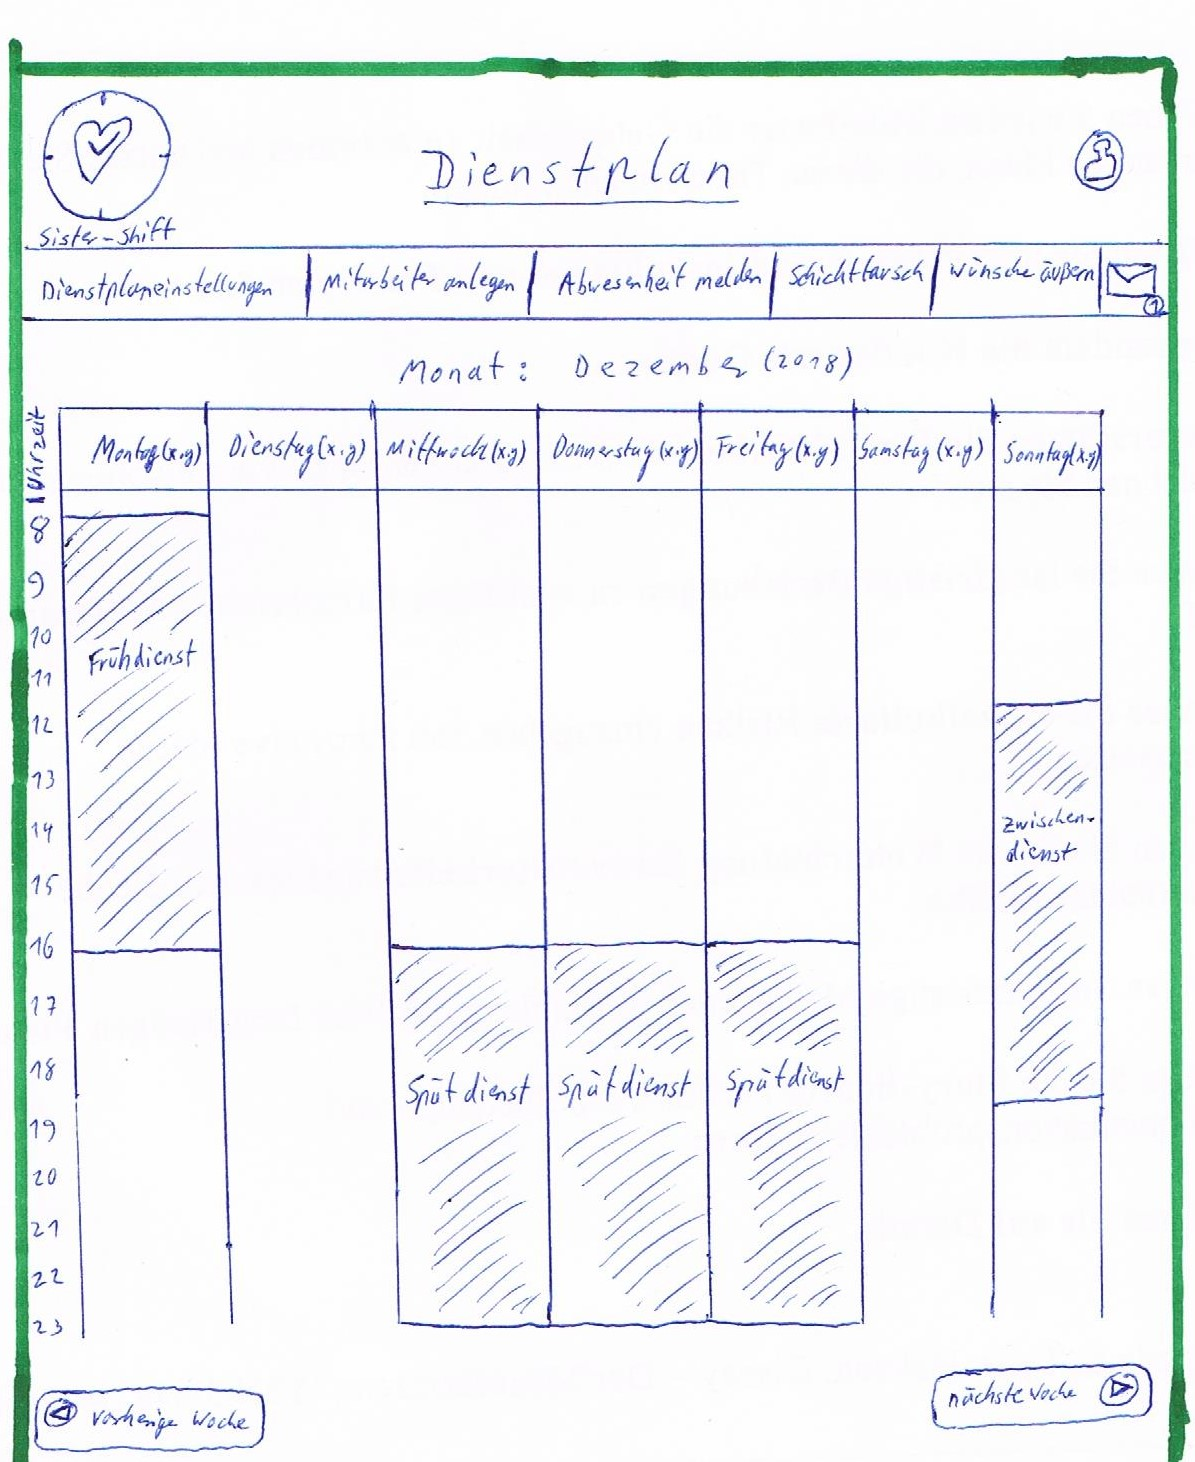
\includegraphics[width=1\textwidth]{Bilder/Wireframe.jpg}
\caption{Wireframe Dienstplan}
\end{figure}
\begin{figure}[H]
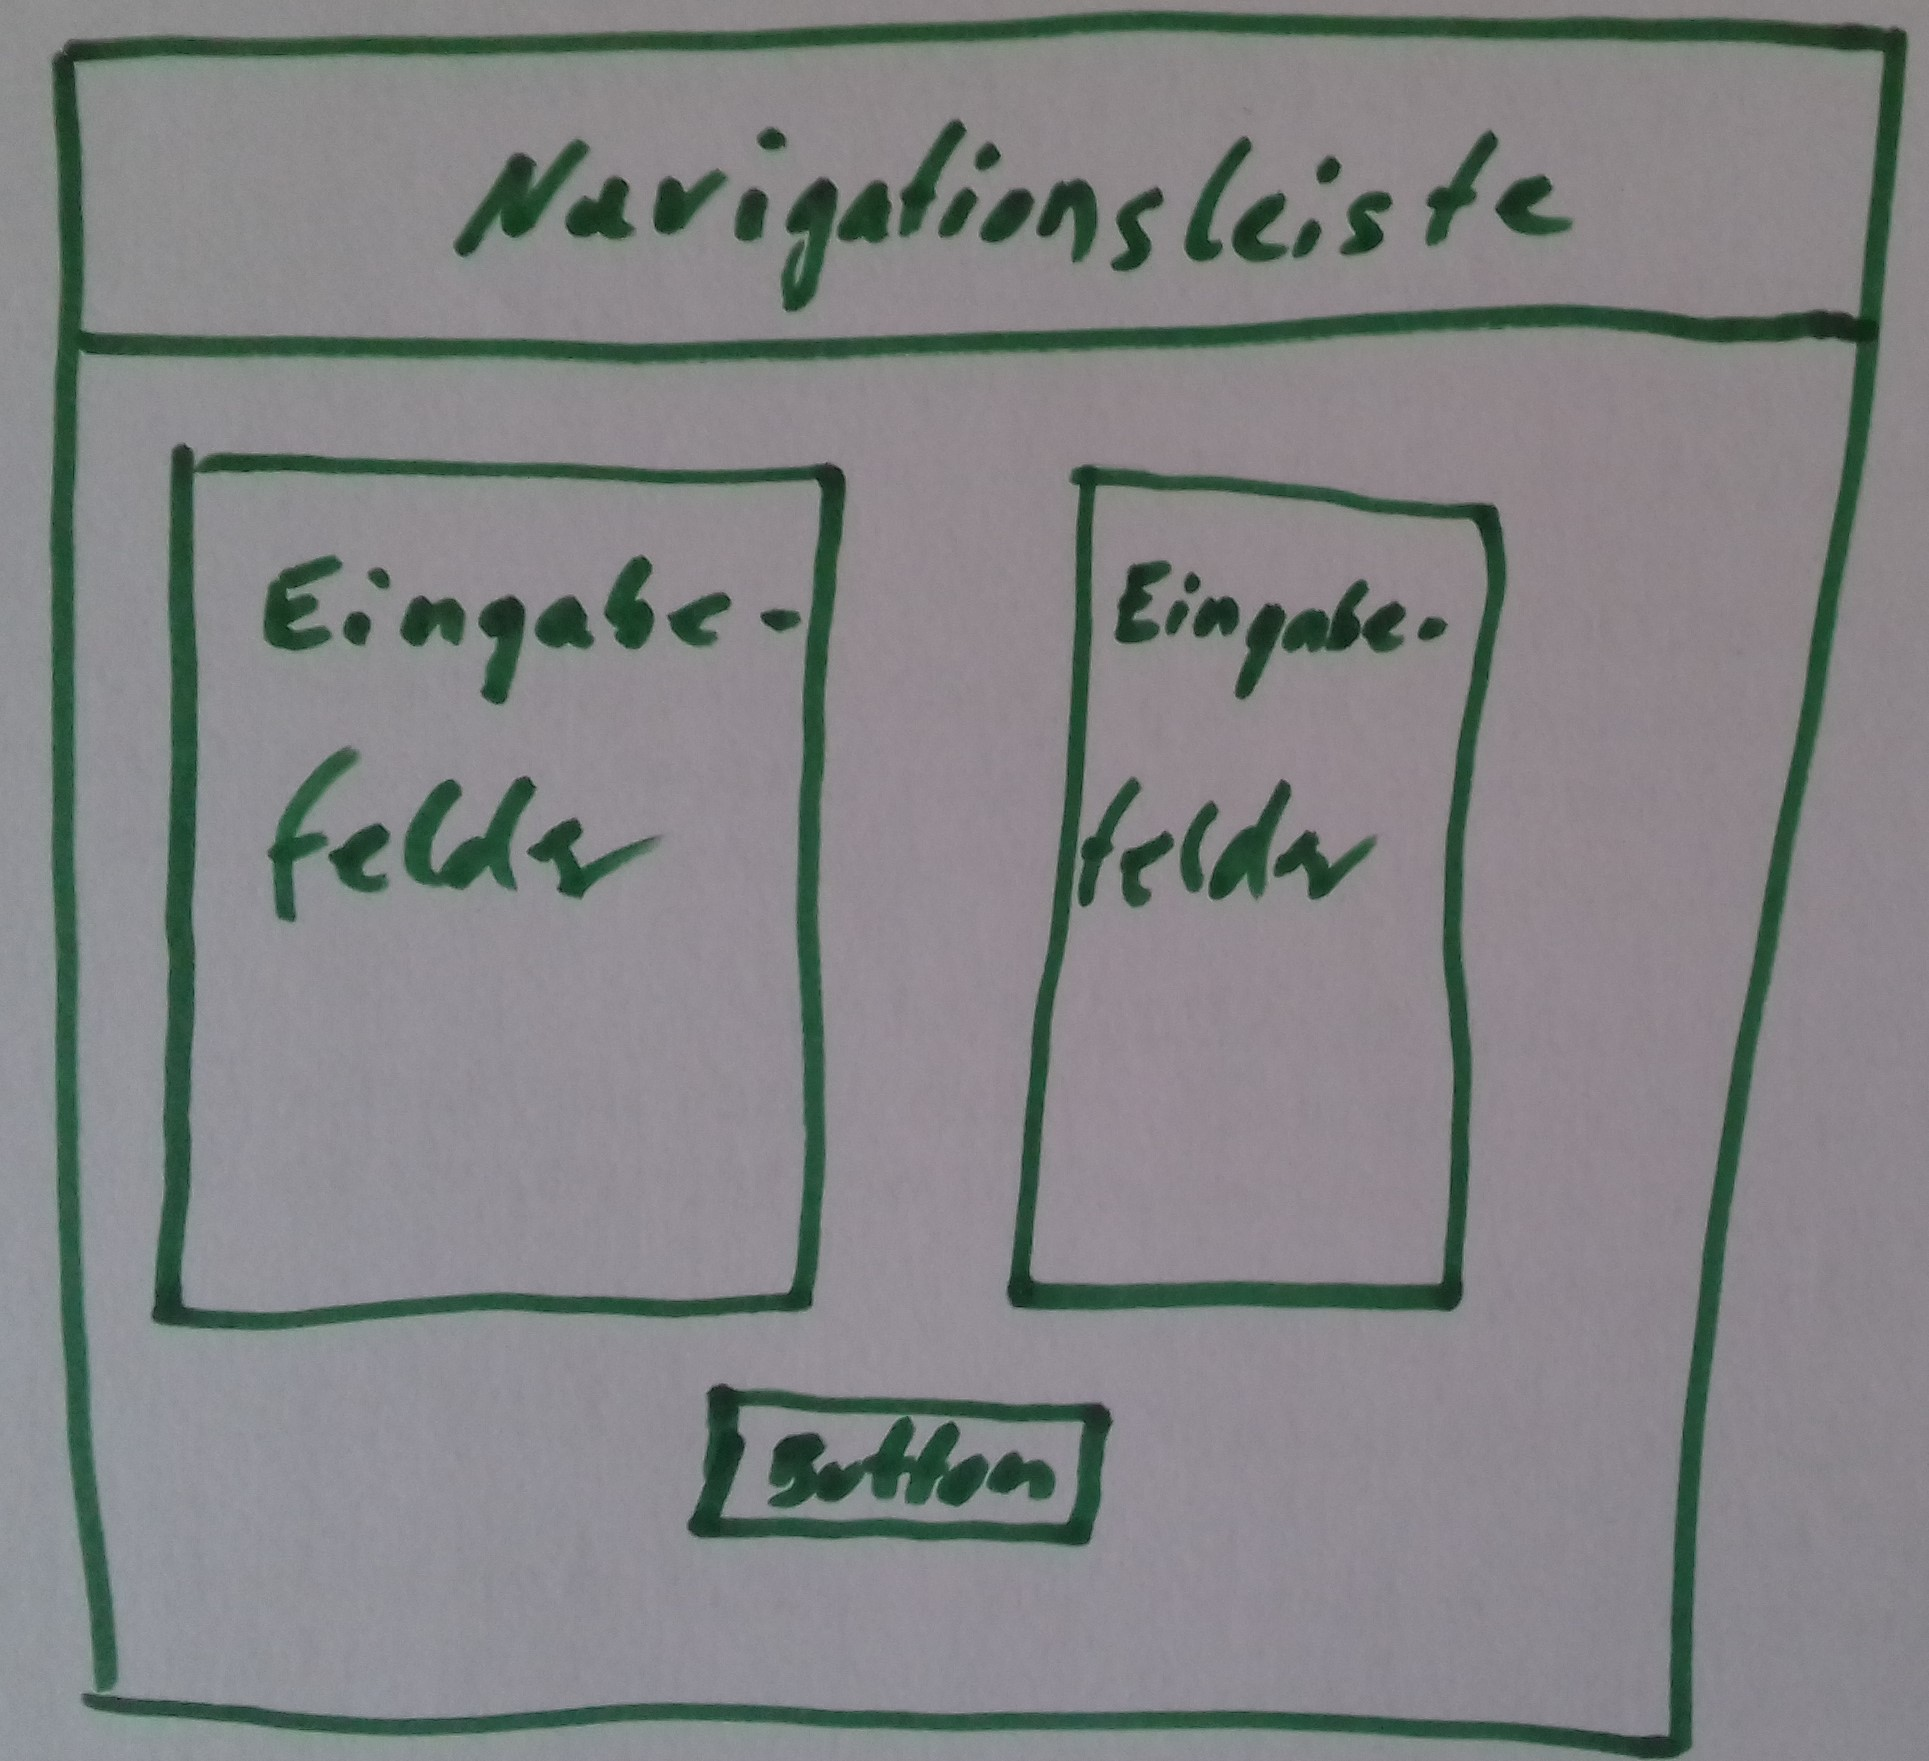
\includegraphics[width=1\textwidth]{Bilder/Wireframe2.jpg}
\caption{Wireframe Sonstige Screens}
\end{figure}
\subsection{Fazit}
Ein konzeptionelles Modell bildet die Grundlage des Designs für das User-Interface. Zusätzlich gibt es einen grundlegende Implementierungsanweisung und dient als Dokumentationsgrundlage. Somit spielt ein konzeptionelles Modell eine wichtige Rolle bei der Entwicklung und vor allem der Gestaltung des Systems.
\section{Mockups}
Ein Mockup ist eine erste Visualisierung der späteren Website. Das Design ist hierbei erst einmal unrelevant. Bei Mockups geht es darum, die verschiedenen Elemente einer Website anzuordnen und somit einen optimalen Userflow zu realisieren. Die Planung der Interaktionsmöglichkeiten und Funktionen der Website steht dabei im Mittelpunkt.
Folgende Ansichten sind auf den erstellten Mockups zu sehen: \\\\
-Login\\
-Dienstplaneinstellungen\\
-Mitarbeiter anlegen/löschen\\
-Dienstplan-Kalender (Hauptfenster)\\
-Schichtdetails\\
-Wunschäußerung, Tauschanfrage und Abwesenheitsmeldung (Zusammengefasst auf Grund des ähnlichen Aufbaus)\\
-Benachrichtigungen\\
-Dialogbox\\
\subsection{Allgemein}
Die Navigation zwischen den einzelnen Funktionen des Systems erfolgt über eine Menüleiste. Diese ist permanent zu sehen und fixiert. Durch Klicken auf das Logo kommt man zurück zur Hauptansicht “Dienstplan - Kalender”. Diese Ansicht ist das Hauptfenster, auf welches der Nutzer auch nach dem erfolgreichen Einloggen gelangt.
\subsection{Login}
Der Login-Screen erfordert nur einen Benutzernamen und das passende Passwort für das genannte Konto. Über einen Login-Button kann sich eingeloggt werden.
\begin{figure}[H]
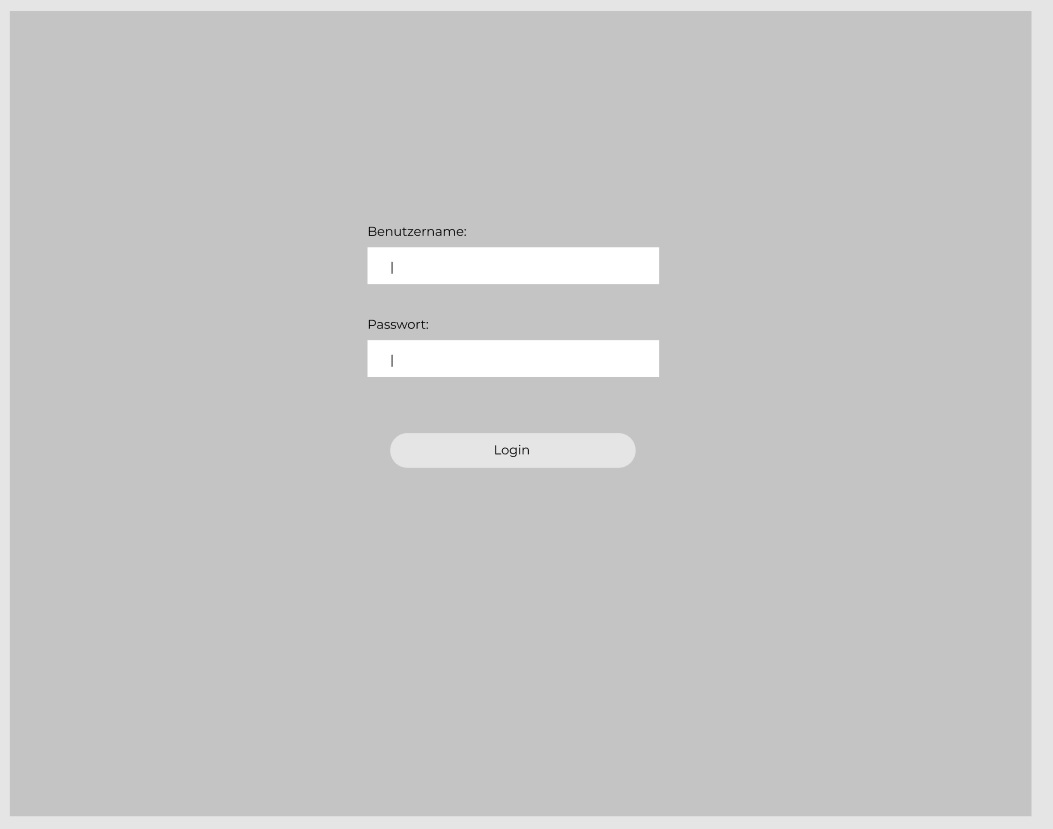
\includegraphics[width=1\textwidth]{Bilder/Login.jpg}
\caption{Login}
\end{figure}
\subsection{Dienstplaneinstellungen}
In dieser Ansicht müssen vor der automatischen Generierung eines Dienstplans die zu sehenden Eckdaten gesetzt werden. Hat der User alle Eckdaten gesetzt, kann durch den Button “Dienstplan generieren” ein neuer Dienstplan vom System generiert werden.
\begin{figure}[H]
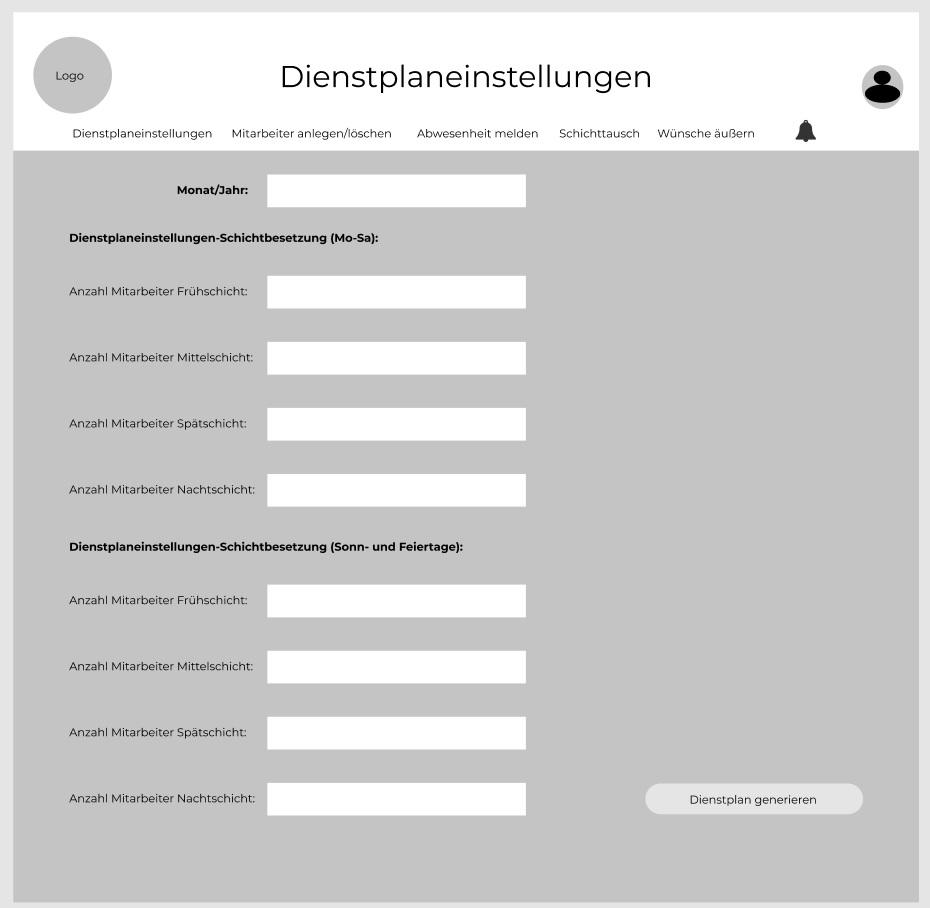
\includegraphics[width=1\textwidth]{Bilder/Dienstplanerstellung.jpg}
\caption{Dienstplanerstellung}
\end{figure}
\subsection{Mitarbeiter anlegen/löschen}
Auf dieser Ansicht kann die Stationsleitung einen neuen Mitarbeiter in das System einpflegen. Dafür müssen die zu sehenden Datenfelder ausgefüllt werden. Zusätzlich kann auch ein Mitarbeiter aus dem System entfernt werden. Die Buttons “Mitarbeiter anlegen” und “Mitarbeiter löschen” bestätigen den jeweiligen Vorgang.
\begin{figure}[H]
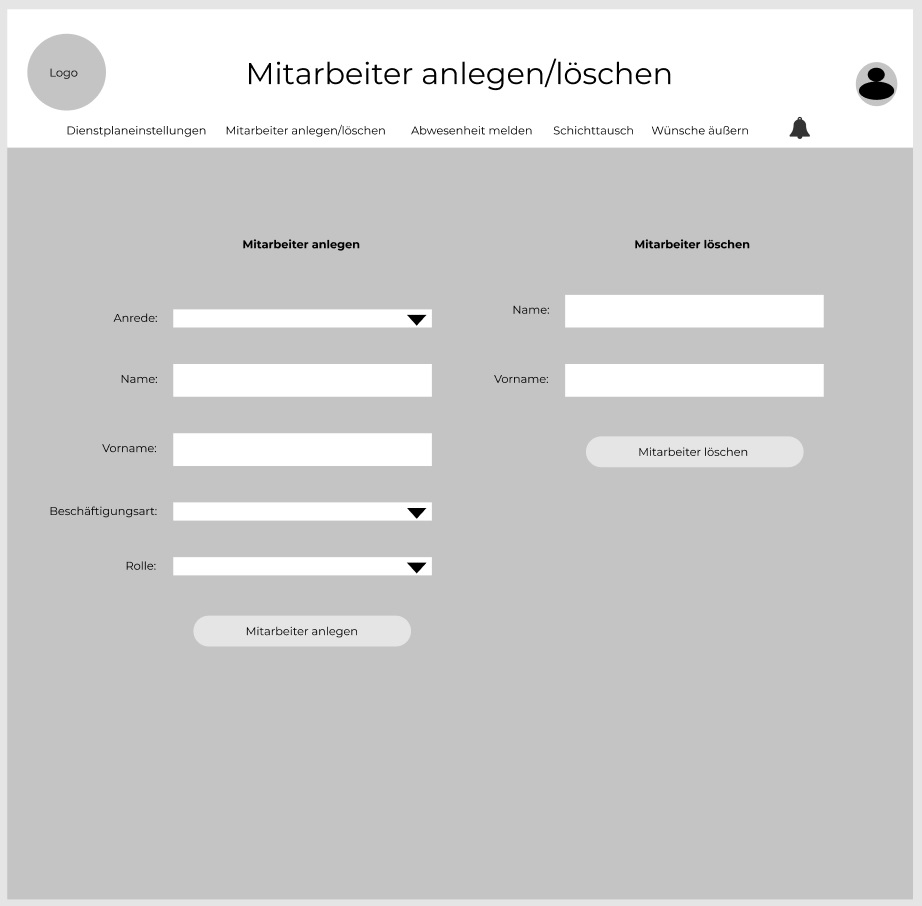
\includegraphics[width=1\textwidth]{Bilder/Mitarbeiteranlegen_loeschen.jpg}
\caption{Mitarbeiter anlegen/löschen}
\end{figure}
\subsection{Dienstplan-Kalender}
In dieser Ansicht kann ein Benutzer den für sich relevanten Dienstplan einsehen. Gezeigt wird immer eine Woche. Über die Buttons “Nächste Woche” und “Vorherige Woche” kann der weitere Dienstplan der anderen Wochen eingesehen werden.
\begin{figure}[H]
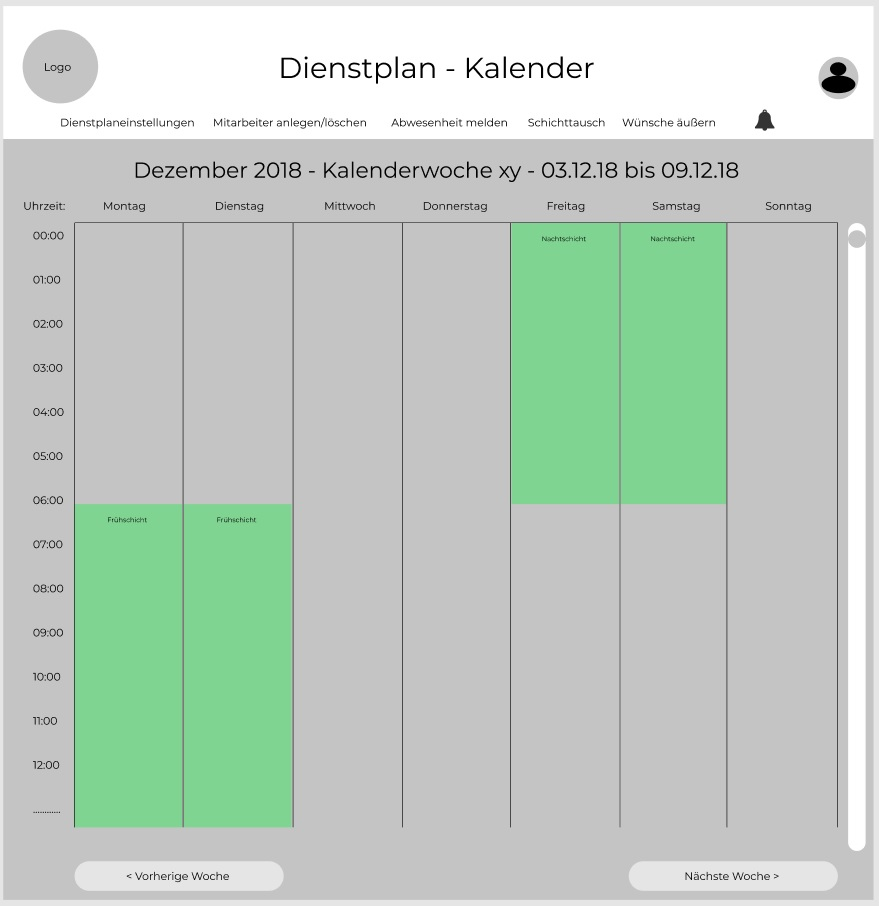
\includegraphics[width=1\textwidth]{Bilder/Dienstplan-Kalender.jpg}
\caption{Dienstplan Kalender}
\end{figure}
\subsection{Schichtdetails}
Zu dieser Ansicht gelangt der Nutzer, sobald er eine Schicht aus der Dienstplan-Kalender Ansicht anklickt. Hier werden Details der betreffenden Schicht angezeigt. Über den Button “Zurück zur Übersicht” gelangt der Nutzer wieder auf die Ansicht des Dienstplan-Kalenders. 
\begin{figure}[H]
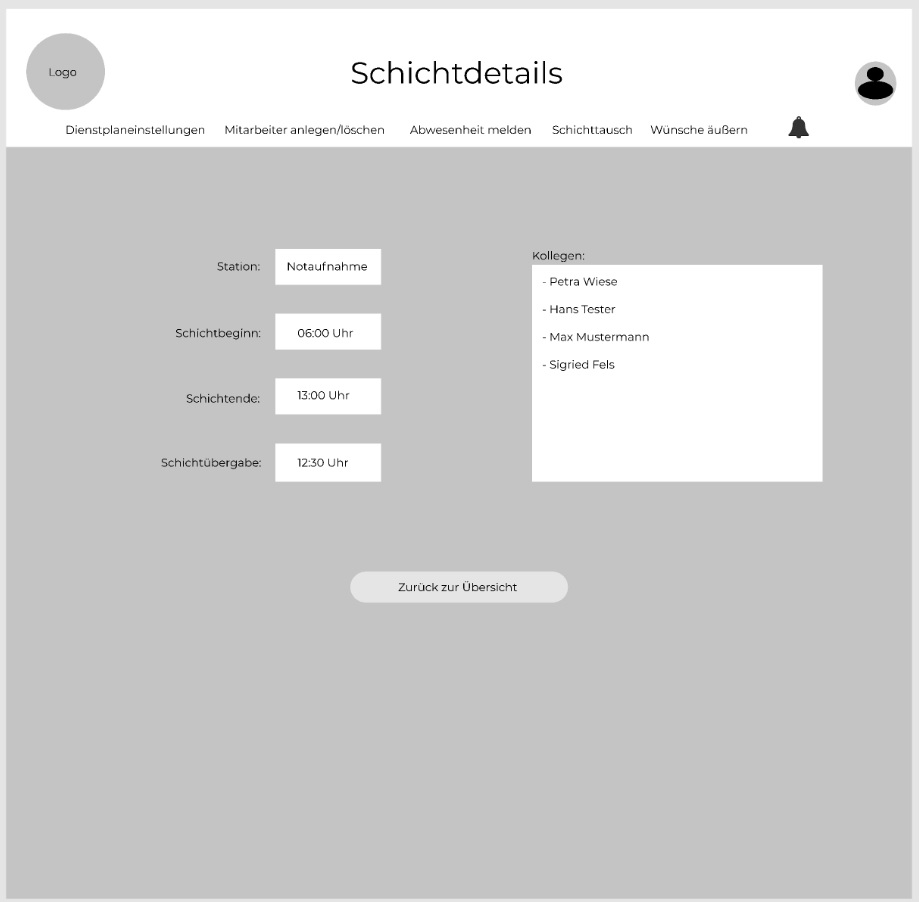
\includegraphics[width=1\textwidth]{Bilder/Schichtdetails.jpg}
\caption{Schichtdetails}
\end{figure}
\subsection{Wunschäußerung, Tauschanfrage und Abwesenheitsmeldung}
Das Mockup dieser drei Ansichten wurde auf Grund der Ähnlichkeiten zusammengefasst. Auf den verschiedenen Ansichten können Wünsche zur weiteren Dienstplanung, Tauschanfragen zu Schichten und Abwesenheitsmeldungen an das System übermittelt werden. Bei jeder dieser Funktionen muss ein Datum und eine Schicht spezifiziert werden. Ausnahmen, bzw. detaillierte Beschreibungen zum Thema Datums- und Schichtangabe bezüglich der jeweiligen Funktion folgt im Kapitel Detailed User Interface. Bei jeder der Funktionen ist die Möglichkeit gegeben einen Kommentar mit an das System zu übermitteln. Über einen entsprechenden Button kann die jeweilige Funktion ausgeführt werden. Bei der Funktion Abwesenheit melden gibt es zusätzlich den Button, der es erlaubt Dokumente, wie z.B. eine Krankmeldung direkt mit anzuhängen. 
\begin{figure}[H]
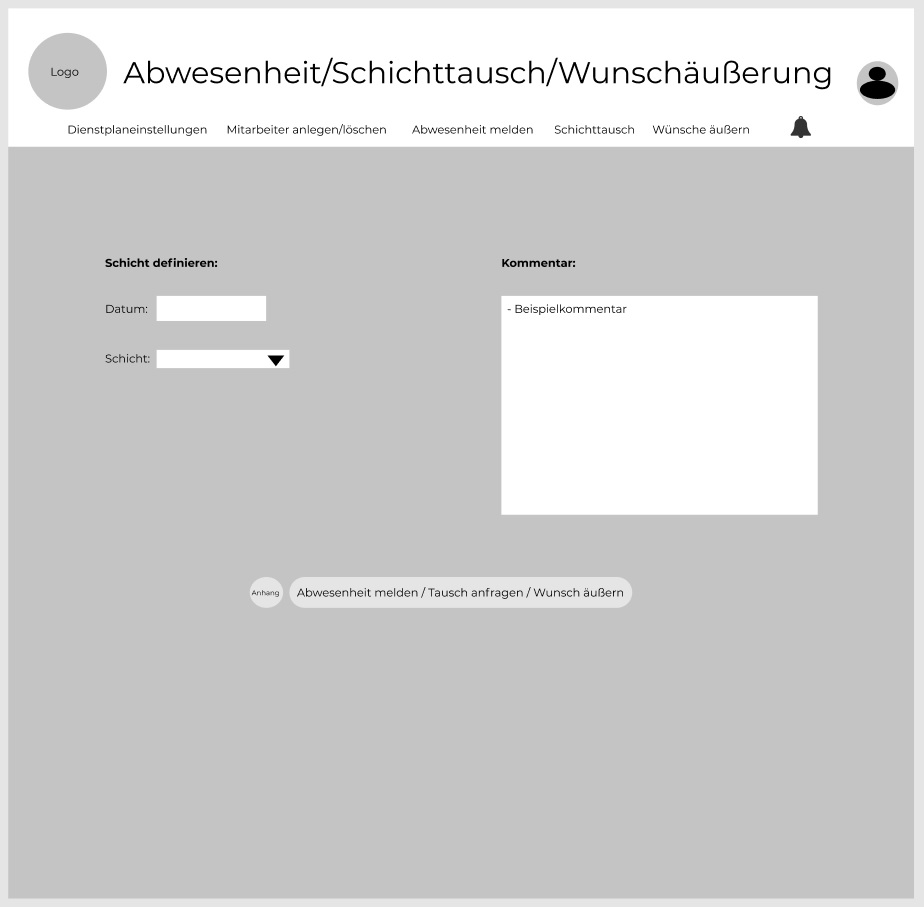
\includegraphics[width=1\textwidth]{Bilder/Abwesenheit_Schichttausch_Wunsch.jpg}
\caption{Diverse Funktionen}
\end{figure}
\subsection{Benachrichtigungen}
Auf dieser Ansicht können die Benachrichtigungen des jeweiligen Nutzers eingesehen werden. Durch Klicken auf das Navigationselement, öffnet sich eine Dialogbox, in der die Nachrichten erscheinen. Klickt man in dieser eine Nachricht an, öffnet sich die gesamte Nachricht nach unten hin in diesem Dialogfenster. Durch den “Schließen”-Button kann man die Dialogbox schließen.
\begin{figure}[H]
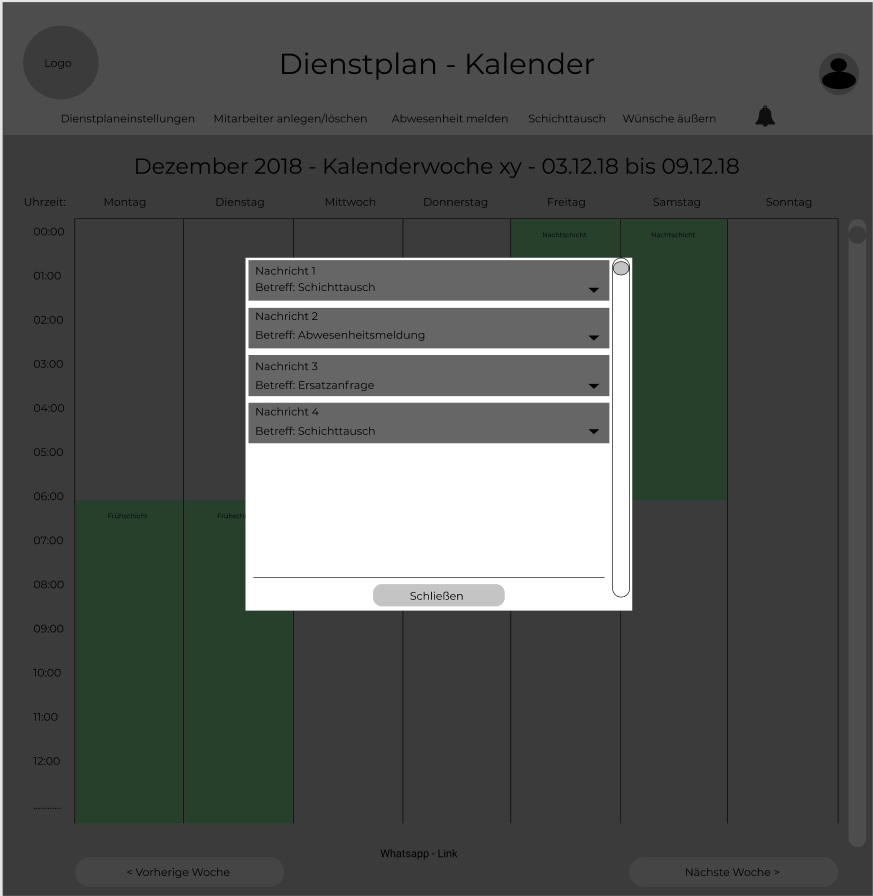
\includegraphics[width=1\textwidth]{Bilder/Benachrichtigungen-Mockup.jpg}
\caption{Benachrichtigungen}
\end{figure}
\subsection{Dialogbox}
Auf dieser Ansicht ist die Anordnung und Gestaltung einer Dialogbox zu sehen. Diese Art des User Feedbacks erfolgt nach dem Ausführen einer vom System bereitgestellten Funktion. Durch Bestätigen mit einem Button, schließt sich die Dialogbox, und der User kann wieder navigieren.
\begin{figure}[H]
\includegraphics[width=1\textwidth]]{Bilder/Dialogbox-Mockup.jpg}
\caption{Dialogbox}
\end{figure}
\section{Screen Design Standards}
Um eine Konsistenz und Einfachheit bei der Gestaltung des User-Interface des Systems sicherzustellen, werden Screen Design Standards benötigt. Die beiden Attribute tragen zur Erhöhung der Benutzerfreundlichkeit und der Erlernbarkeit bei. Laut Mayhew erwarten die Benutzer des Systems eine Konsistenz und sind anfällig für Fehlerhaftes Verhalten, falls Inkonsistenzen auftreten.
\subsection{Kontrollelemente Standards}
Menü-/Navigationsleiste\\\\
Die Primärnavigation im System erfolgt über die Navigationsleiste. Diese befindet sich immer am oberen Rand der Webseite.\\\\
Buttons\\\\
Mit Buttons können verschiedene Aktionen und Funktionen vom Benutzer ausgelöst werden. Beispielsweise das Einreichen einer Abwesenheitsmeldung erfolgt nach der Angabe aller erforderlichen Daten über einen Button. Die Buttons befinden sich immer am unteren Rand der Webseite, unter dem Hauptinhalt. \\\\
Textfelder\\\\
Damit der Nutzer diverse Texteingaben tätigen kann, werden Textfelder eingesetzt. Die Möglichkeit auf eine Texteingabe ist z.B. beim Äußern eines Wunsches zum nächsten Dienstplan möglich. \\\\
Datumsfelder\\\\
Datumsfelder werden für den Benutzer zur Eingabe verschiedener Daten benutzt. Dies ist z.B. bei der Meldung einer Abwesenheit sehr wichtig. \\\\
Dropdown-Menü\\\\
Bei User-Eingaben, bei denen es nur eine sehr begrenzte, und festgeschriebene Anzahl an Auswahlmöglichkeiten gibt, wird ein Dropdown-Menü verwendet.\\\\
Kalender\\\\
Der Kalender des Hauptfensters, in dem der Dienstplan einzusehen ist, bietet eine gewisse Kontrollfunktion. Er gewährleistet dies, indem der Inhalt dieses anklickbar ist. Durch Klicken auf eine Schicht, kann ein Nutzer die jeweiligen Schichtdetails einsehen.\\\\
\subsection{Layout Standards}
Das Layout von Designelementen ist durch die Nutzung des Frameworks Semantic UI auf den Stil dieses beschränkt. Dazu gehören z.B. die Elemente Navigationsleiste, Buttons, Schrift, Textfelder und ähnliches.
\subsection{Interaktionsstandards}
Das System hat gewisse Interaktionsstandards, welche im Folgenden festgelegt werden. Der Nutzer hat die gezeigten Interaktionsmöglichkeiten: \\\\

1. Klicken: \\\\
Der Nutzer kann alle oben genannten Kontrollelemente anklicken, um die entsprechenden Funktionen auszuführen. Dies geschieht durch das klicken der linken Maustaste. \\\\
2. Schreiben:\\\\
Der Nutzer kann durch die Tastatur in der Anwendung schreiben. Beispielsweise kann er so, das Kommentarfeld bei der Funktion ‘Schichttausch’ ausfüllen. Vor dem Schreiben muss das jeweilige Element durch Klicken ausgewählt werden. \\\\
3. Informationen senden:\\\\
Der Nutzer sendet nach einem Schichttausch oder einer Abwesenheit Benachrichtigungen an die Stationsleitung über die Änderungen. Dies geschieht automatisch und ohne Nutzerinteraktion.\\\\
4. Benachrichtigungen bearbeiten:\\\\
Die Benutzer des Systems erhalten verschiedene Benachrichtigungen. Handelt es sich nicht nur um ein Statusupdate zur Personalplanung, so handelt es sich um Ersatzanfragen. Diese können durch Klicken auf die jeweilige Nachricht und auf dem entsprechenden Screen eingesehen und bearbeitet werden. Ersatzanfragen werden durch Klicken bestätigt oder abgelehnt.
\subsection{Feedback Standards}
Feedback Standards bilden eine Art Antwort für den Nutzer. Dies erfolgt z.B. bei einer erfolgreichen Eingabe. Folgende Standards bietet das System:\\\\
1. Dialogboxen:\\\\
Dialogboxen legen sich über die aktuelle Webseite um Informationen anzuzeigen, oder eine Userinteraktion zu erzwingen. Die Informationsdarstellung kann jeglicher Form entsprechen. Die Dialogboxen haben Buttons, die der Nutzerinteraktion dienen. Diese Art von Feedback erfolgt nach jeder erfolgreichen Ausführung einer der vom System angebotenen Funktionen. Der User erhält somit ein direktes Feedback zur Ausführung. Das Feedback soll in der Form von Dialogboxen erfolgen, da der Nutzer so aufgefordert ist, die Informationen des Systems zu lesen, bevor dieser eine weitere Aktion ausführen kann.\\\\
2. Aktives Menüelement:\\\\
Die vom Nutzer aktuell ausgewählte Seite wird als Überschrift in der Navigationsleiste verwendet. Zusätzlich wird der aktive Menüpunkt besonders hervorgehoben. Somit weiß der Nutzer immer auf welcher Seite er sich gerade befindet.\\\\
3. Aktualisierung Kontrollelement:\\\\
Durch Klicken auf einen Interaktionsbutton verändert und aktualisiert sich ein Element der Webseite. Dies gewährt dem Nutzer direktes Feedback. Bei der Kalenderübersicht des Dienstplans ist dies der Fall, wenn der Nutzer durch die verschiedenen Wochen eines Monats blättert.
\subsection{Responsive Design}
Ein responsives Webdesign passt sich automatisch der Größe und Auflösung des aktuellen Endgeräts an. Es verändert einzelne Elemente, wie z.B. die Navigationsleiste und passt diese der jeweiligen Größe an. HTML 5 und CSS3 sind moderne Webstandards, welche die technische Basis dafür bieten. Das verwendete Framework Sementic UI setzt bereits entsprechende Techniken um, und ist somit für responsives Webdesign ausgelegt und ausgestattet. Durch ein responsives Design kann die Anwendung Sister-Shift auch von verschiedenen Endgeräten genutzt werden, solange diese einen internetfähigen Webbrowser aufweisen.
\subsection{Effizienz und Geschwindigkeit}
Die Effizienz und Geschwindigkeit werden durch die Verwendung von AJAX stark verbessert. AJAX bietet Möglichkeit Informationen auf einer Webseite nur partiell zu aktualisieren. Ein Laden der gesamten Seite wird damit vermieden. Dadurch wird die Dauer der Ladevorgänge minimiert und ermöglicht den Nutzern eine schnellere Benutzung der Anwendung. Dies ist bei der Aktualisierung des Dienstplan-Kalenders sehr wichtig.
\subsection{Dokumentation}
Die Navigation und die Nutzung der Funktionen der Webseite sollen ohne weitere Dokumentation oder Hilfestellungen erfolgen können. 
\subsection{Fazit}
Die formulierten Standards erleichtern das Erreichen von Konsistenz und Einfachheit im finalen Design. Die Standards ersparen bei der späteren Entwicklung viel Zeit.
\section{Detailed User Interface}
Das System ist als eine Webapplikation umgesetzt. Somit kann diese mit einem Webbrowser der eigenen Wahl geöffnet und bedient werden. Folgend werden die Identifizierten Ansichten im finalen und detaillierten User Interface gezeigt. Es wurden stets die Screen Design Standards und Vorgaben aus dem Styleguide beachtet und umgesetzt.
\subsection{Login}
\begin{figure}[H]
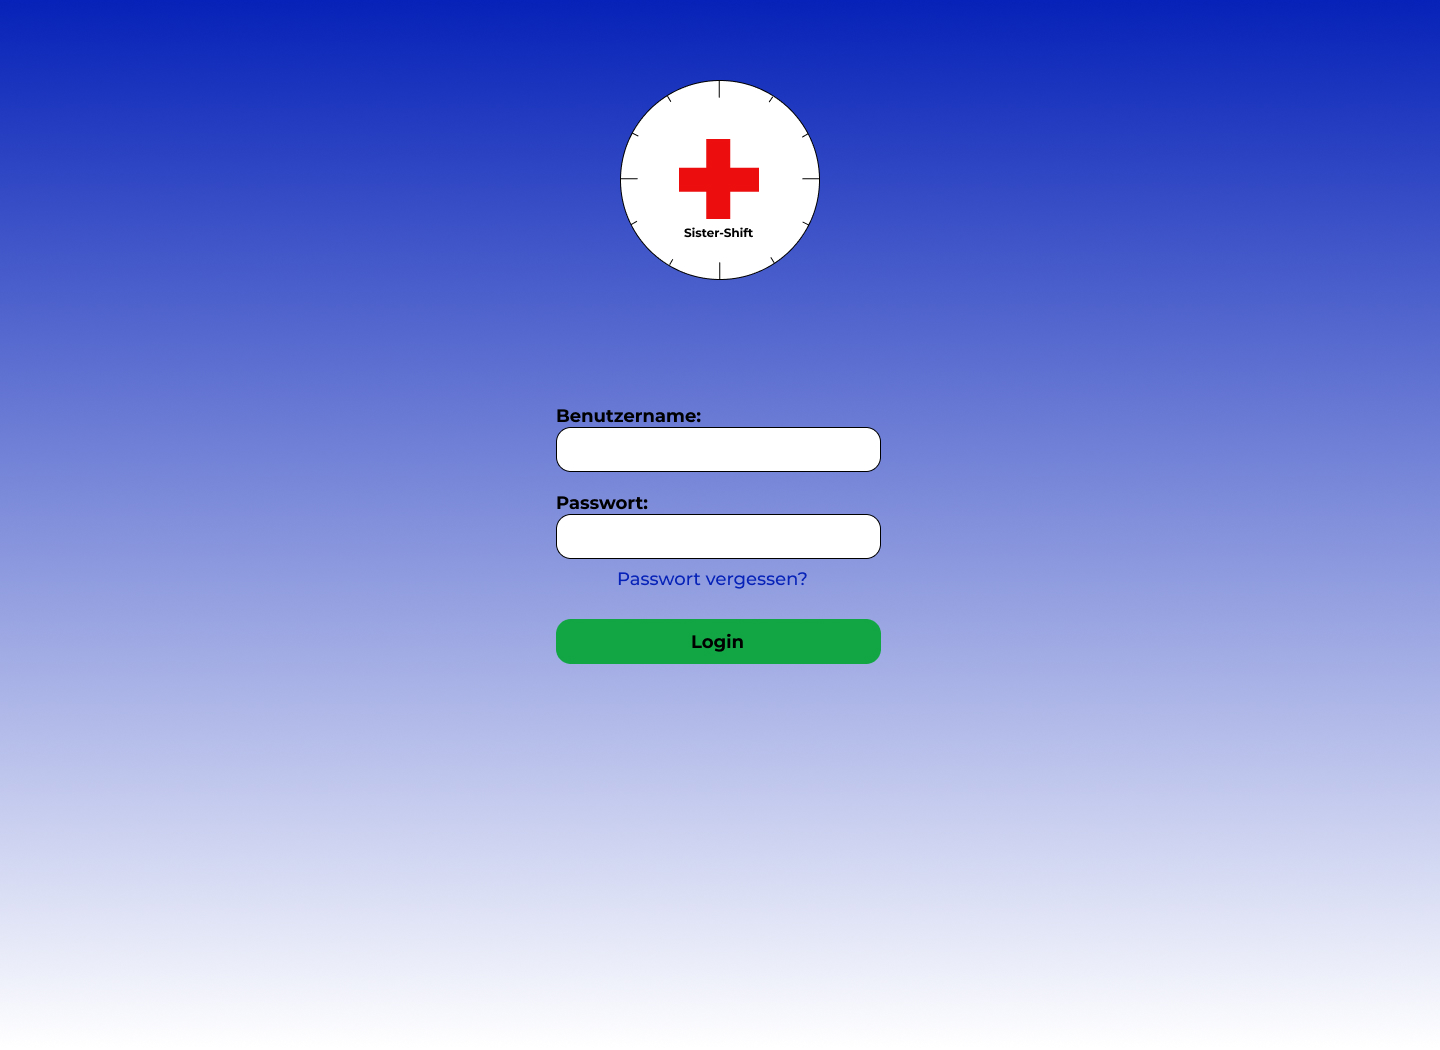
\includegraphics[width=1\textwidth]{Bilder/Screens/Login-Screen.jpg}{\centering}
\caption{Login-Screen}
\end{figure}
Der Login Screen ist sehr einfach und in den Farben der vorher im Styleguide festgelegten Farben gehalten. Durch erfolgreiches einloggen gelangt der jeweilige Benutzer zur Dienstplanübersicht.
\subsection{Dienstplan – Kalender (Hauptansicht)}
\begin{figure}[H]
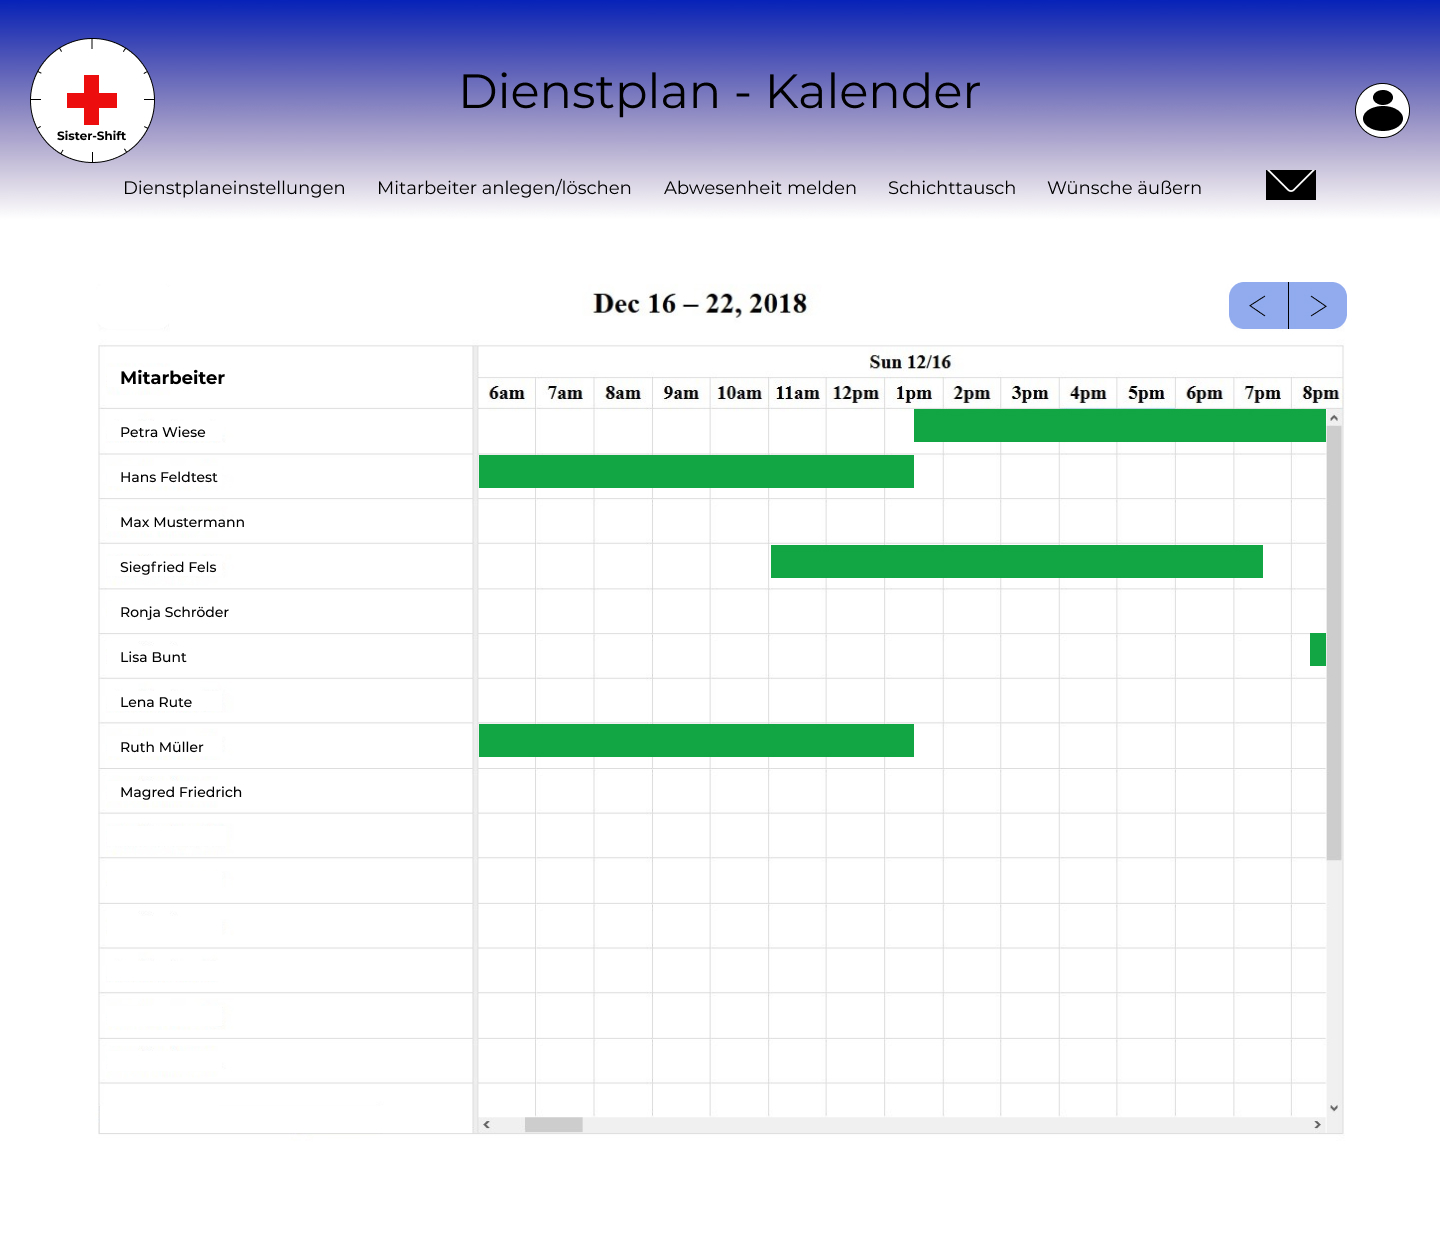
\includegraphics[width=1\textwidth]{Bilder/Screens/Hauptfenster-Kalender.jpg}{\centering}
\caption{Dienstplan Kalender}
\end{figure}
Auf dem Hauptscreen können die Benutzer Ihren Dienstplan einsehen. Dieser ist in Wochen unterteilt. Durch die Buttons können die Wochen durchgeschaltet werden. Die einzelnen Tage der Woche kann ein Nutzer durch scrollen nach Links oder Recht im Kalender einsehen. Schichten, in denen ein Mitarbeiter eingeteilt ist, sind in der im Styleguide gesetzten Sekundärfarbe eingefärbt. In diesen Kalender werden automatisch Schichten vom System eingetragen, gelöscht und hinzugefügt. Die einzelnen Schichten sind anklickbar. Durch auswählen einer Schicht gelangt der User zu den Schichtdetails.
\begin{figure}[H]
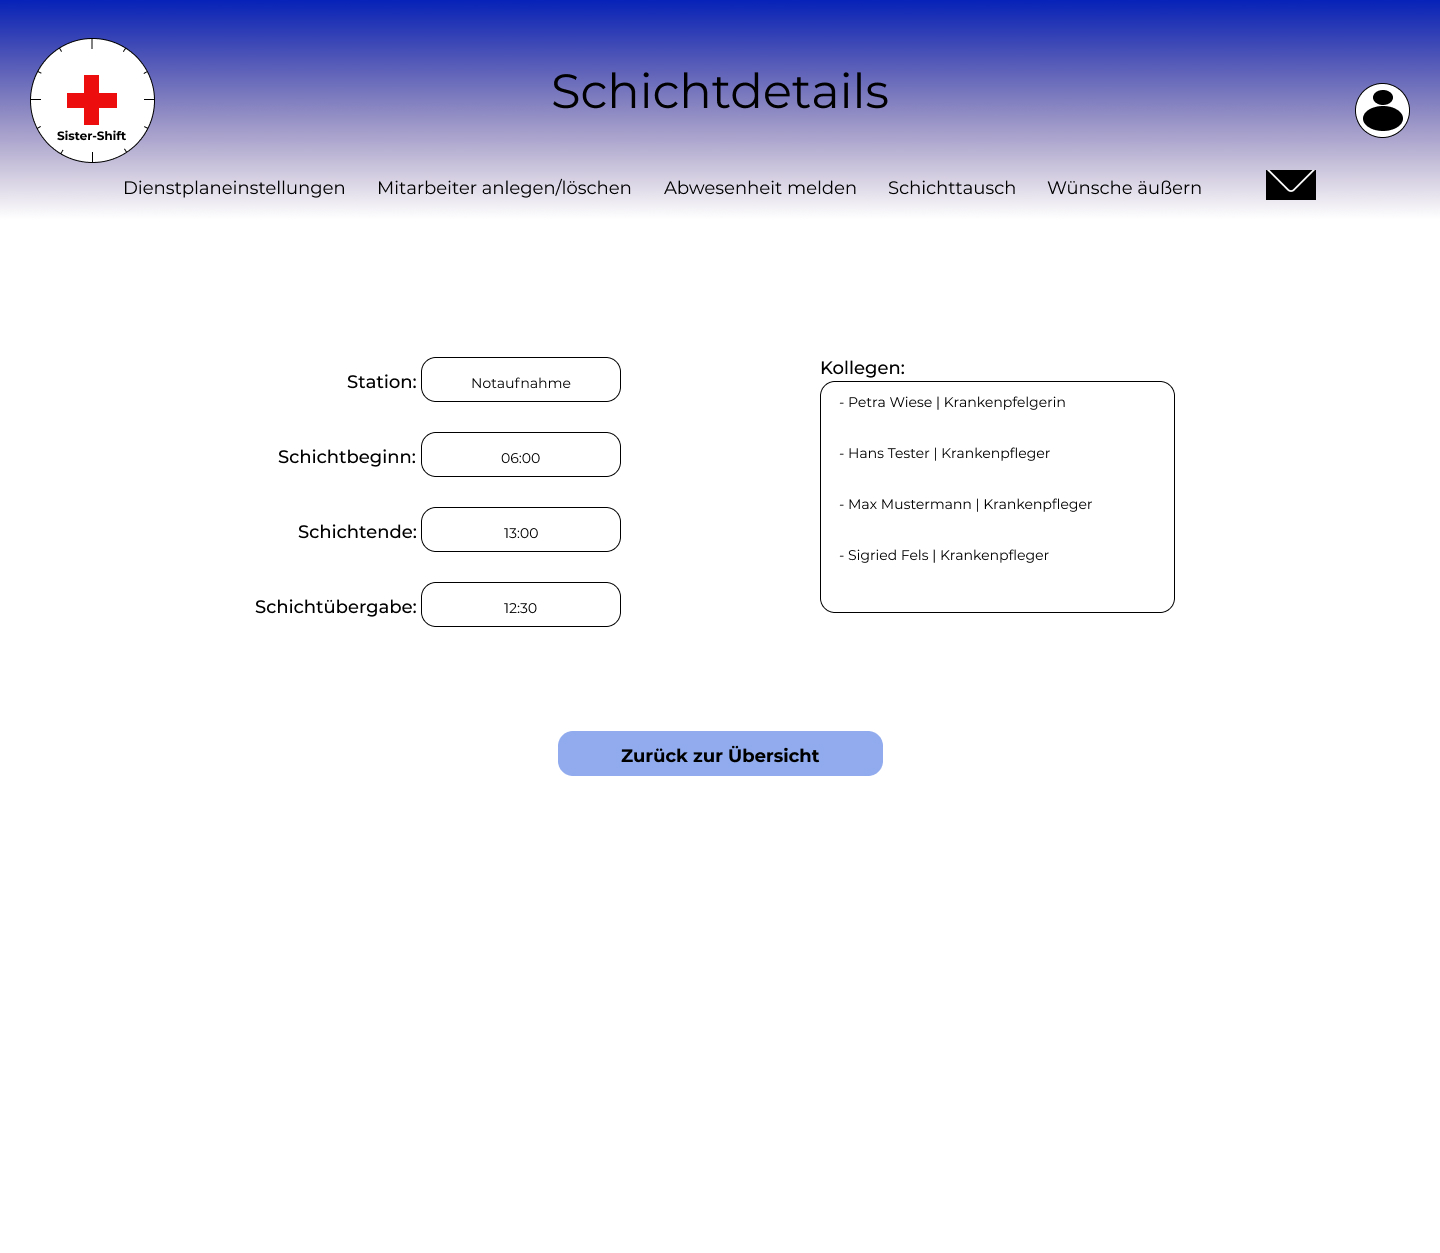
\includegraphics[width=1\textwidth]{Bilder/Screens/Schichtdetails.jpg}{\centering}
\caption{Schichtdetails-Screen}
\end{figure}
Durch das Klicken auf den Button ‘Zurück zur Übersicht’ gelangt der User wieder auf den Dienstplan-Kalender-Screen. Zu sehen ist außerdem die Navigations- beziehungsweise Menüleiste. Durch Klicken auf das Logo der Anwendung gelangt der Benutzer immer auf den Dienstplan-Kalender-Screen. Die anderen Menüpunkte bilden Funktionen des Systems ab. Durch Klicken auf diese gelangt man zu den jeweiligen Screens. ‘Dienstplaneinstellungen’ und ‘Mitarbeiter anlegen/löschen’ sind nur für die Stationsleitung zugänglich.  Es erfolgt eine entsprechende Information, falls ein anderer Benutzer versucht die Funktionen auszuführen. 
\begin{figure}[H]
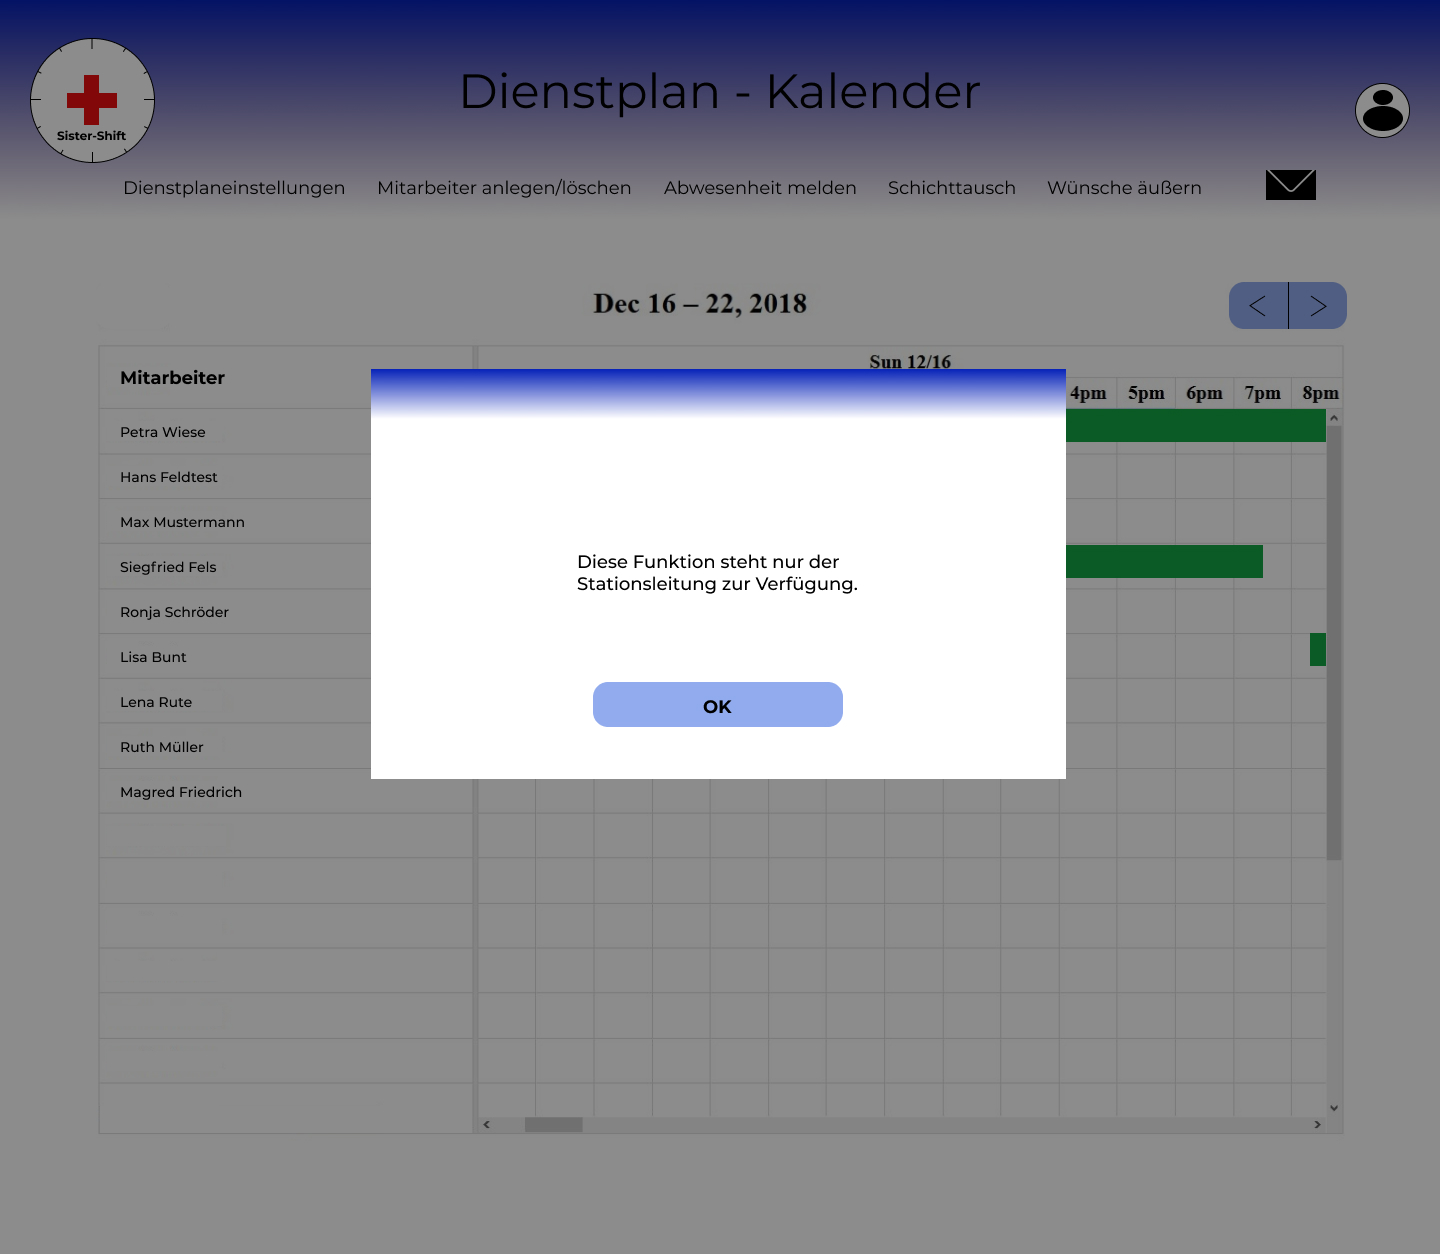
\includegraphics[width=1\textwidth]{Bilder/Screens/Hauptfenster-Kalender-Nutzungsrechte.jpg}{\centering}
\caption{Dialogbox Information Nutzungsrecht}
\end{figure}
Die zu sehenden Icons sind zum einen für Benachrichtigungen (Brief-Icon) und für Benutzerkontoeinstellungen (User-Icon) zuständig. Ungelesene Nachrichten werden durch eine Rote Zahl am Brief-Icon angezeigt.
\begin{figure}[H]
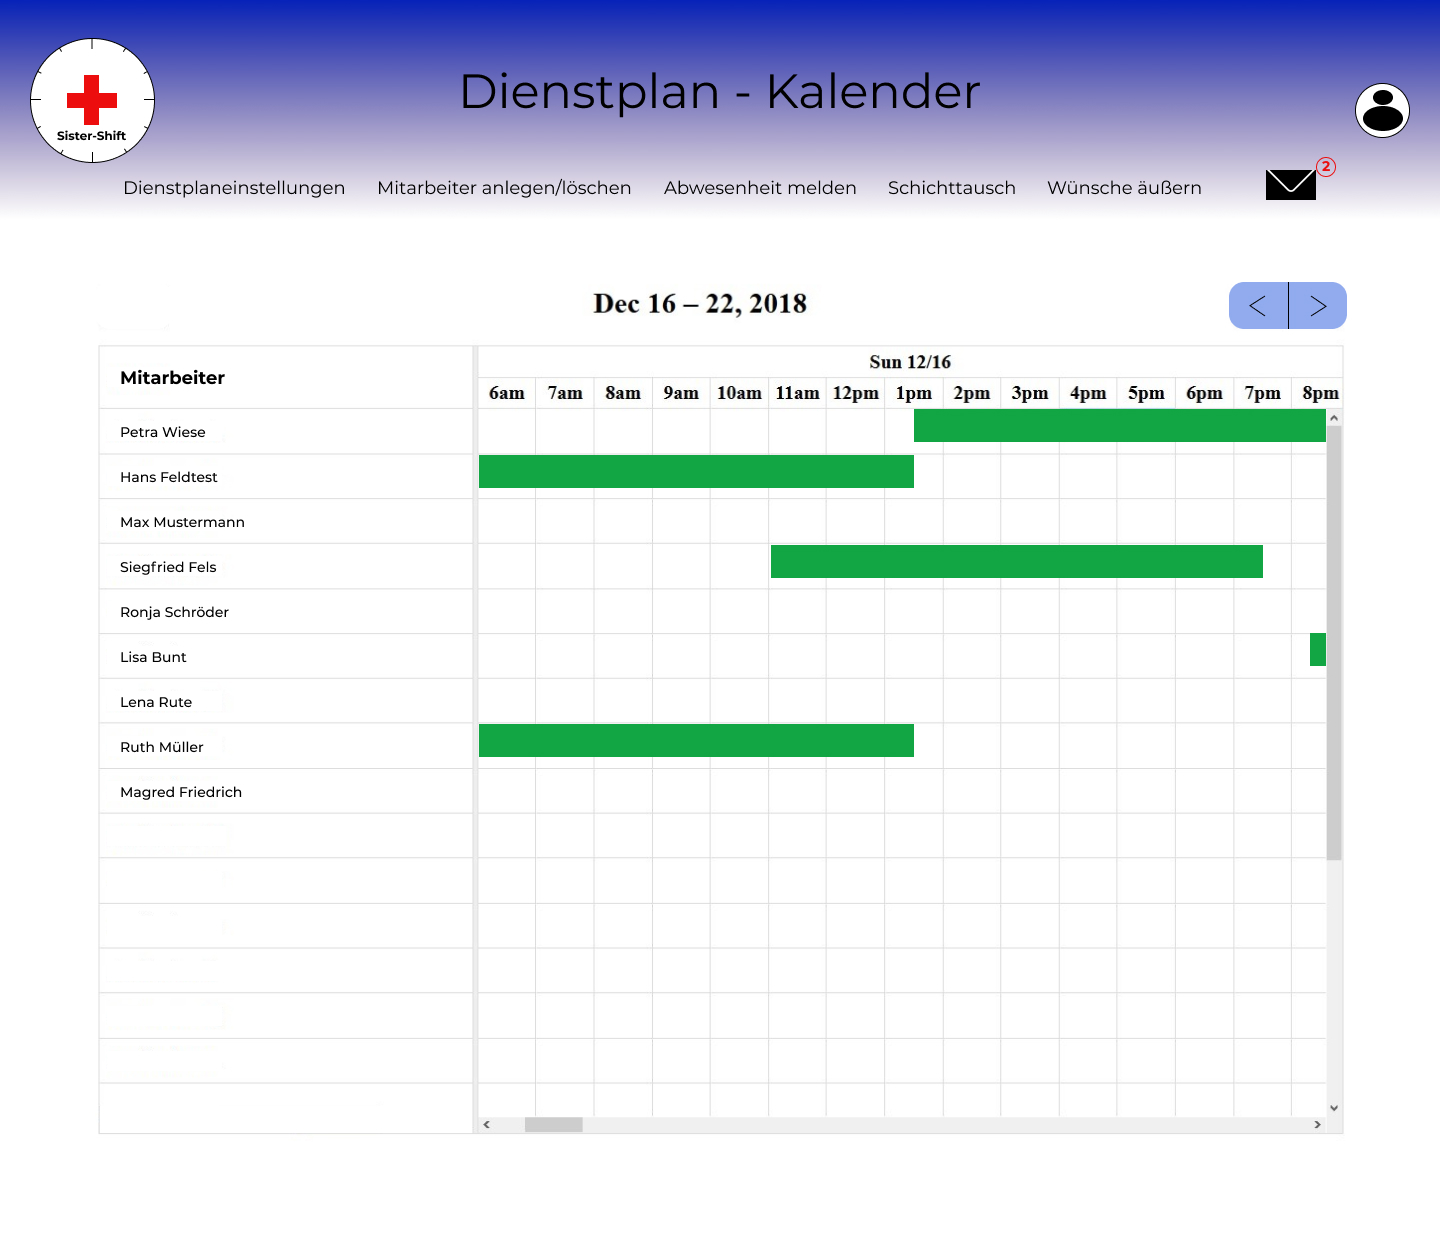
\includegraphics[width=1\textwidth]{Bilder/Screens/Hauptfenster-Kalendermit2Nachrichten.jpg}{\centering}
\caption{Hauptfenster - Kalender mit 2 Nachrichten
}
\end{figure}
Durch Klicken auf das Benachrichtigungs-Icon öffnet sich eine Dialogbox, welche alle Benachrichtigungen mit dem jeweiligen Betreff anzeigt. 
\begin{figure}[H]
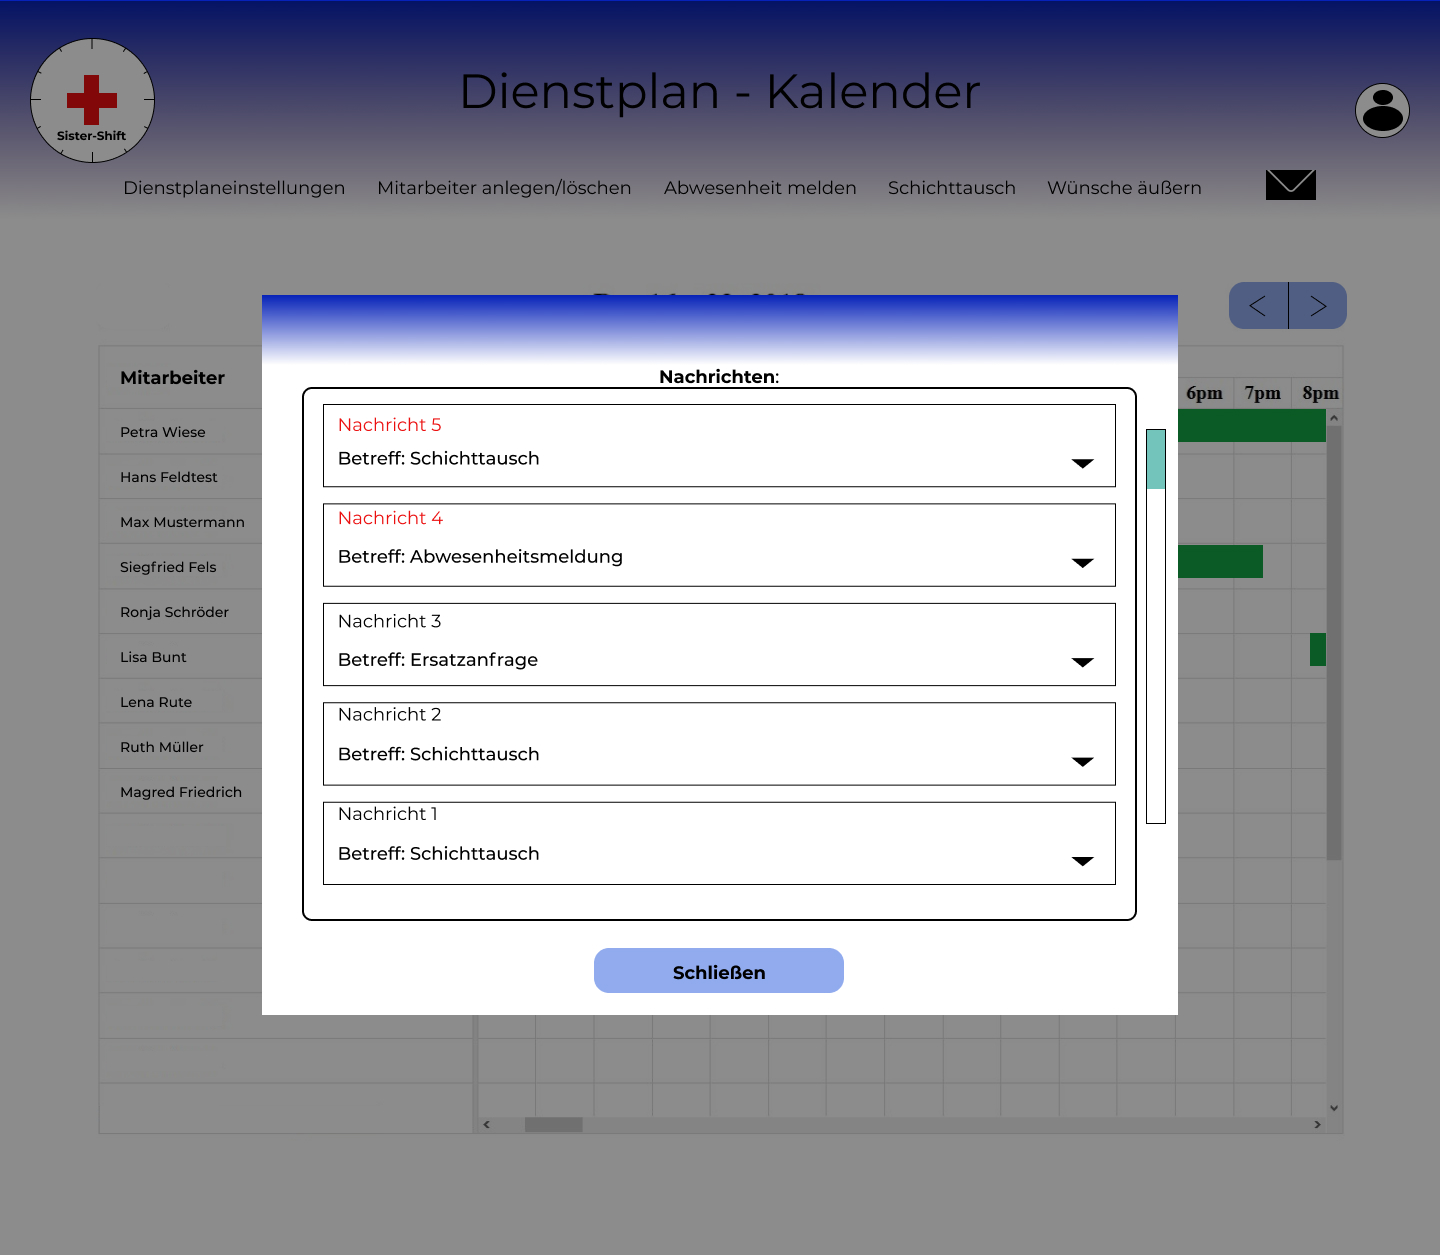
\includegraphics[width=1\textwidth]{Bilder/Screens/Benachrichtigungen-Screen.jpg}{\centering}
\caption{Benachrichtigungen}
\end{figure}
Durch Klicken auf eine Nachricht, klappt diese sich in Richtung unterer Bildschirmrand hin aus und der Benutzer kann diese lesen. Es folgen die verschiedenen Nachrichtentypen, die ein Benutzer mit der Rolle Gesundheits- und Krankenpfleger oder Medizinischer Fachangestellter erhalten kann.
\begin{figure}[H]
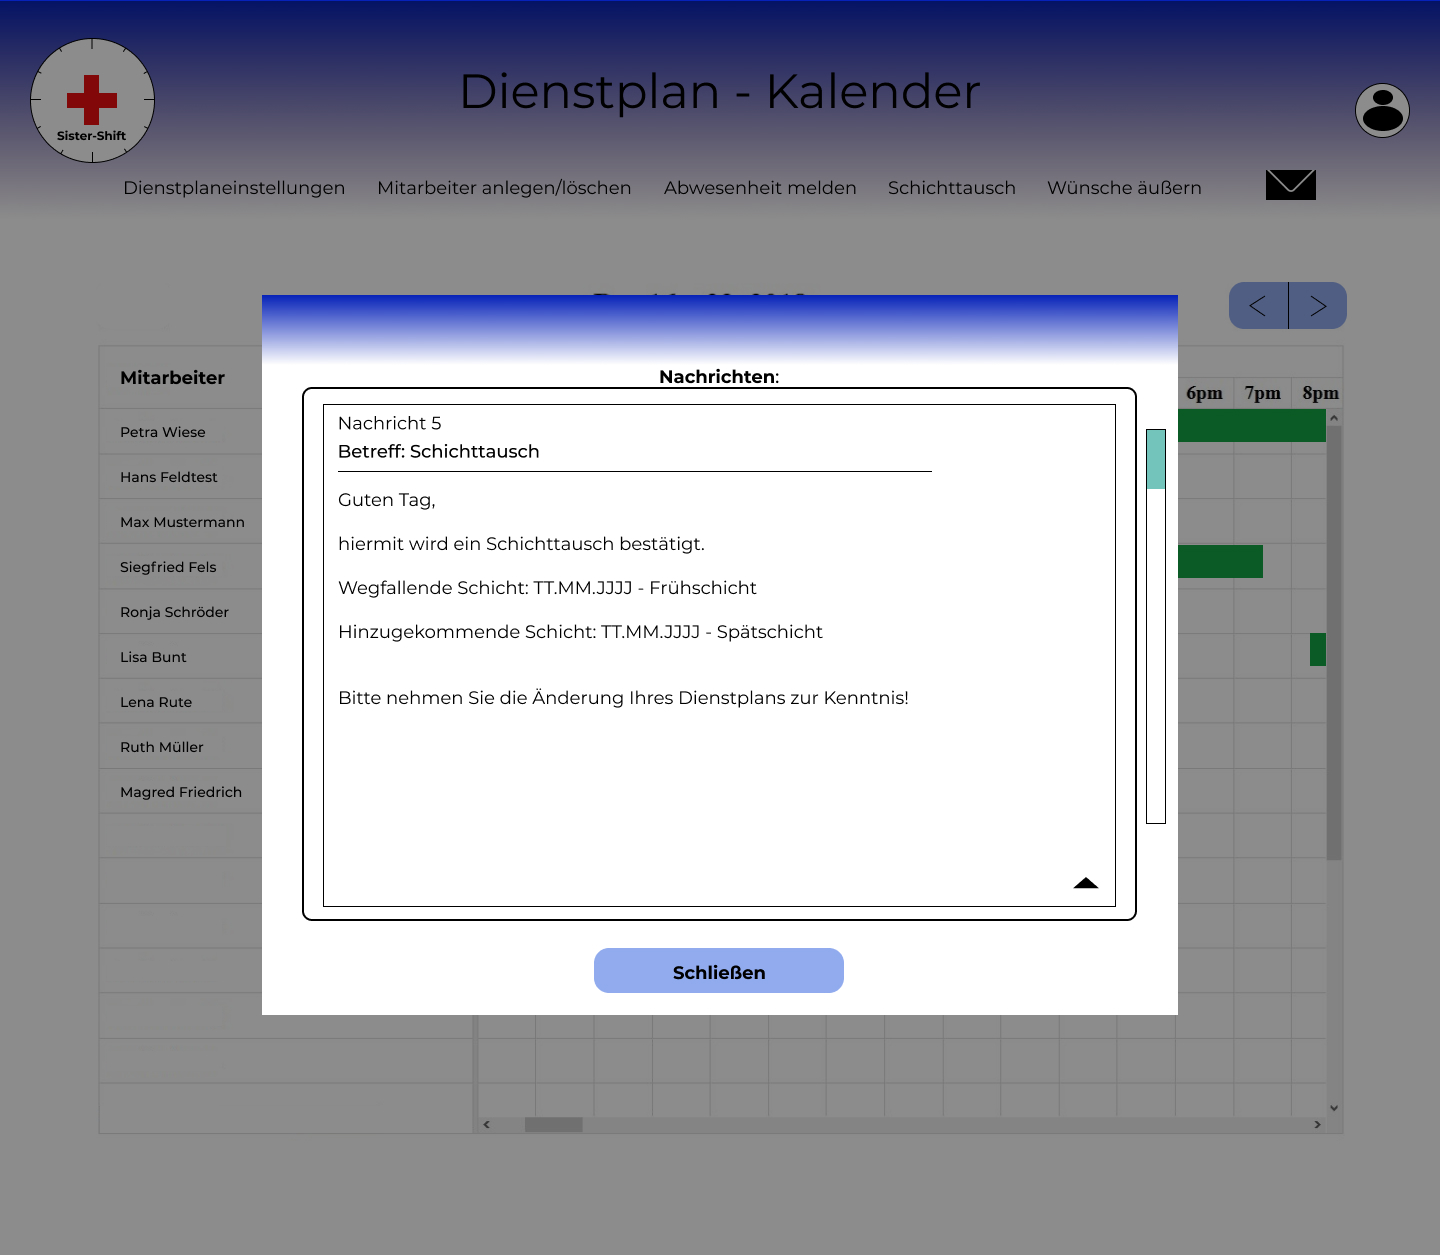
\includegraphics[width=1\textwidth]{Bilder/Screens/NachrichtKrankenpflegerSchichttausch.jpg}{\centering}
\caption{Nachricht Schichttausch}
\end{figure}
\begin{figure}[H]
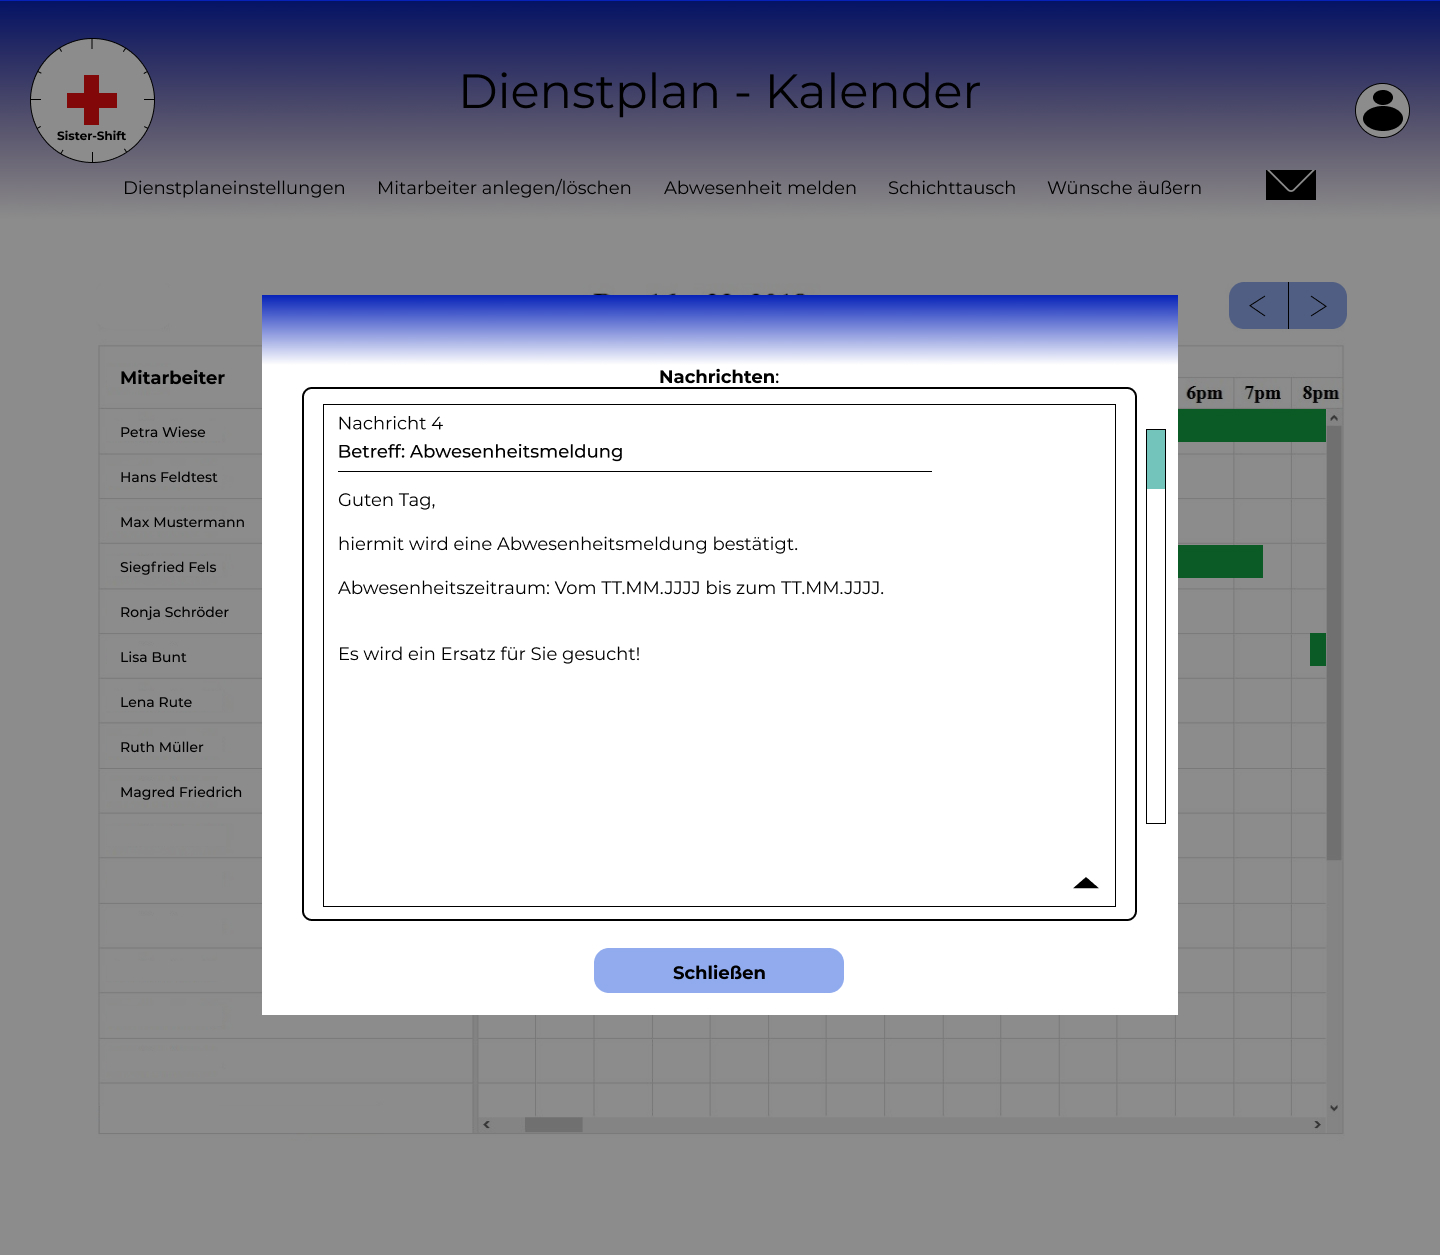
\includegraphics[width=1\textwidth]{Bilder/Screens/NachrichtKrankenpflegerAbwesenheitsmeldung.jpg}{\centering}
\caption{Nachricht Abwesenheitsmeldung}
\end{figure}
\begin{figure}[H]
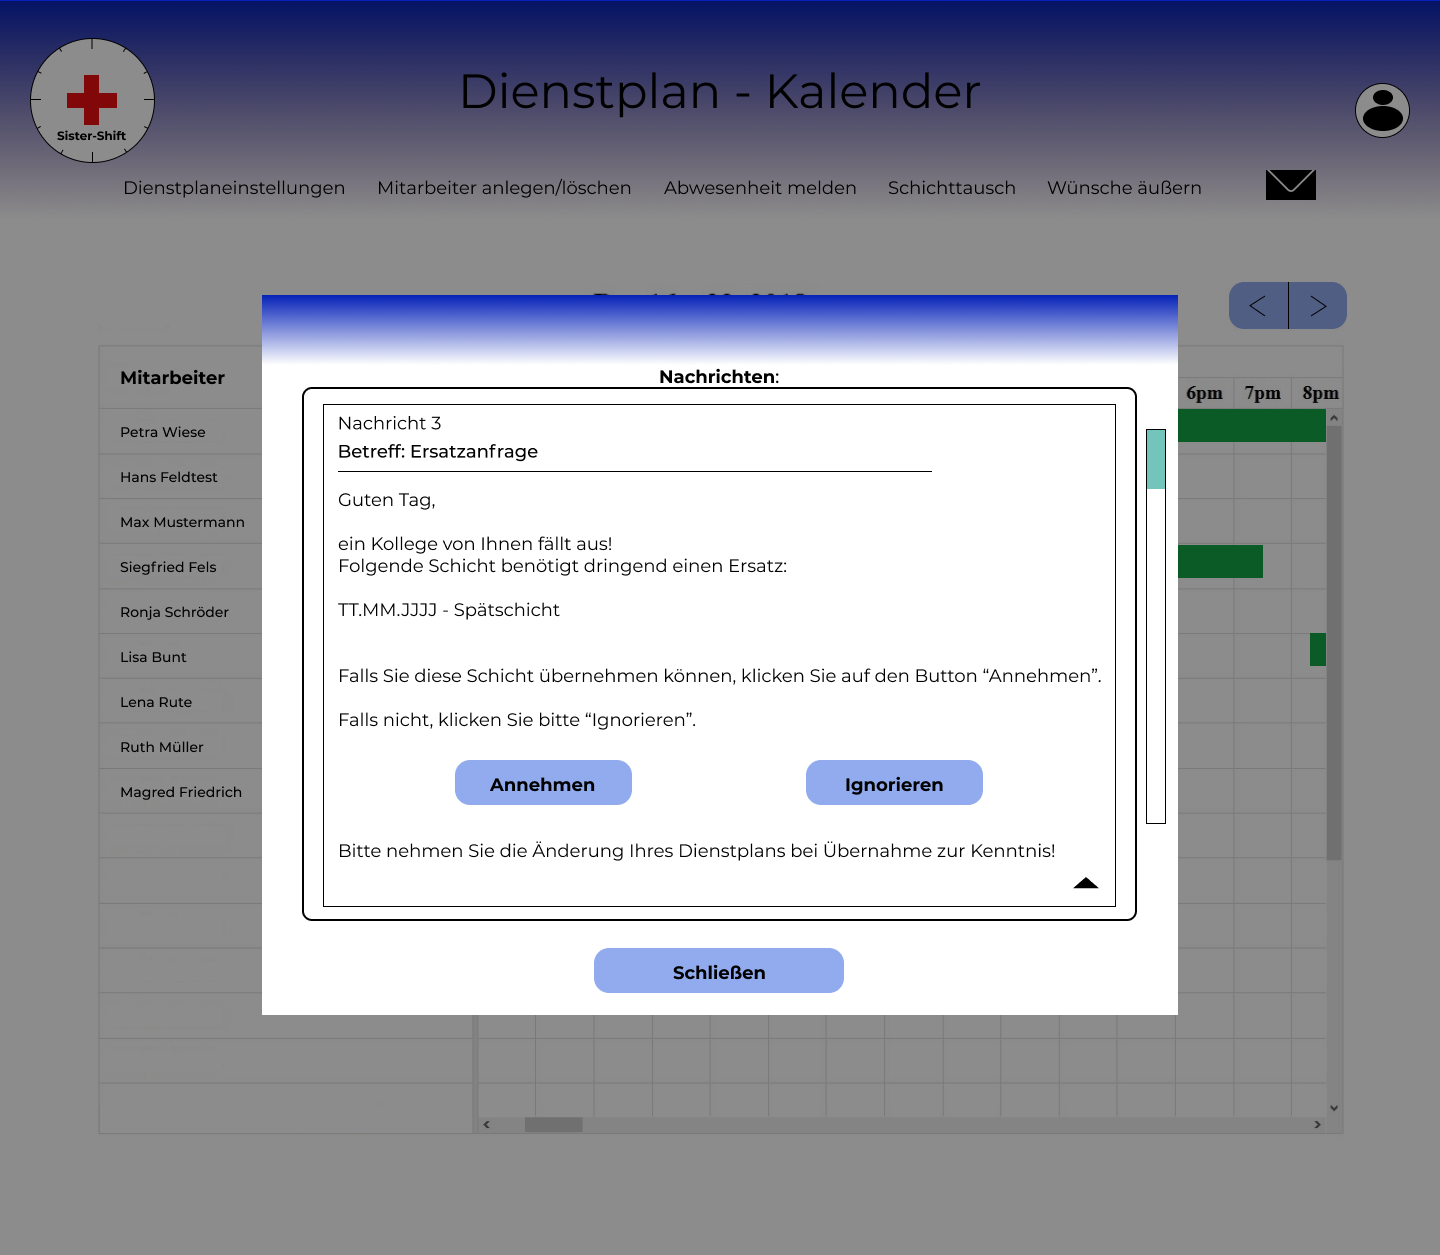
\includegraphics[width=1\textwidth]{Bilder/Screens/NachrichtKrankenpflegerErsatzanfrage.jpg}{\centering}
\caption{Nachricht Ersatzanfrage}
\end{figure}
Durch Klicken auf ‘Annehmen’ oder ‘Ignorieren’ wird die Entscheidung dem System mitgeteilt und für den User durch einfärben des jeweiligen Buttons deutlich gemacht.
\begin{figure}[H]
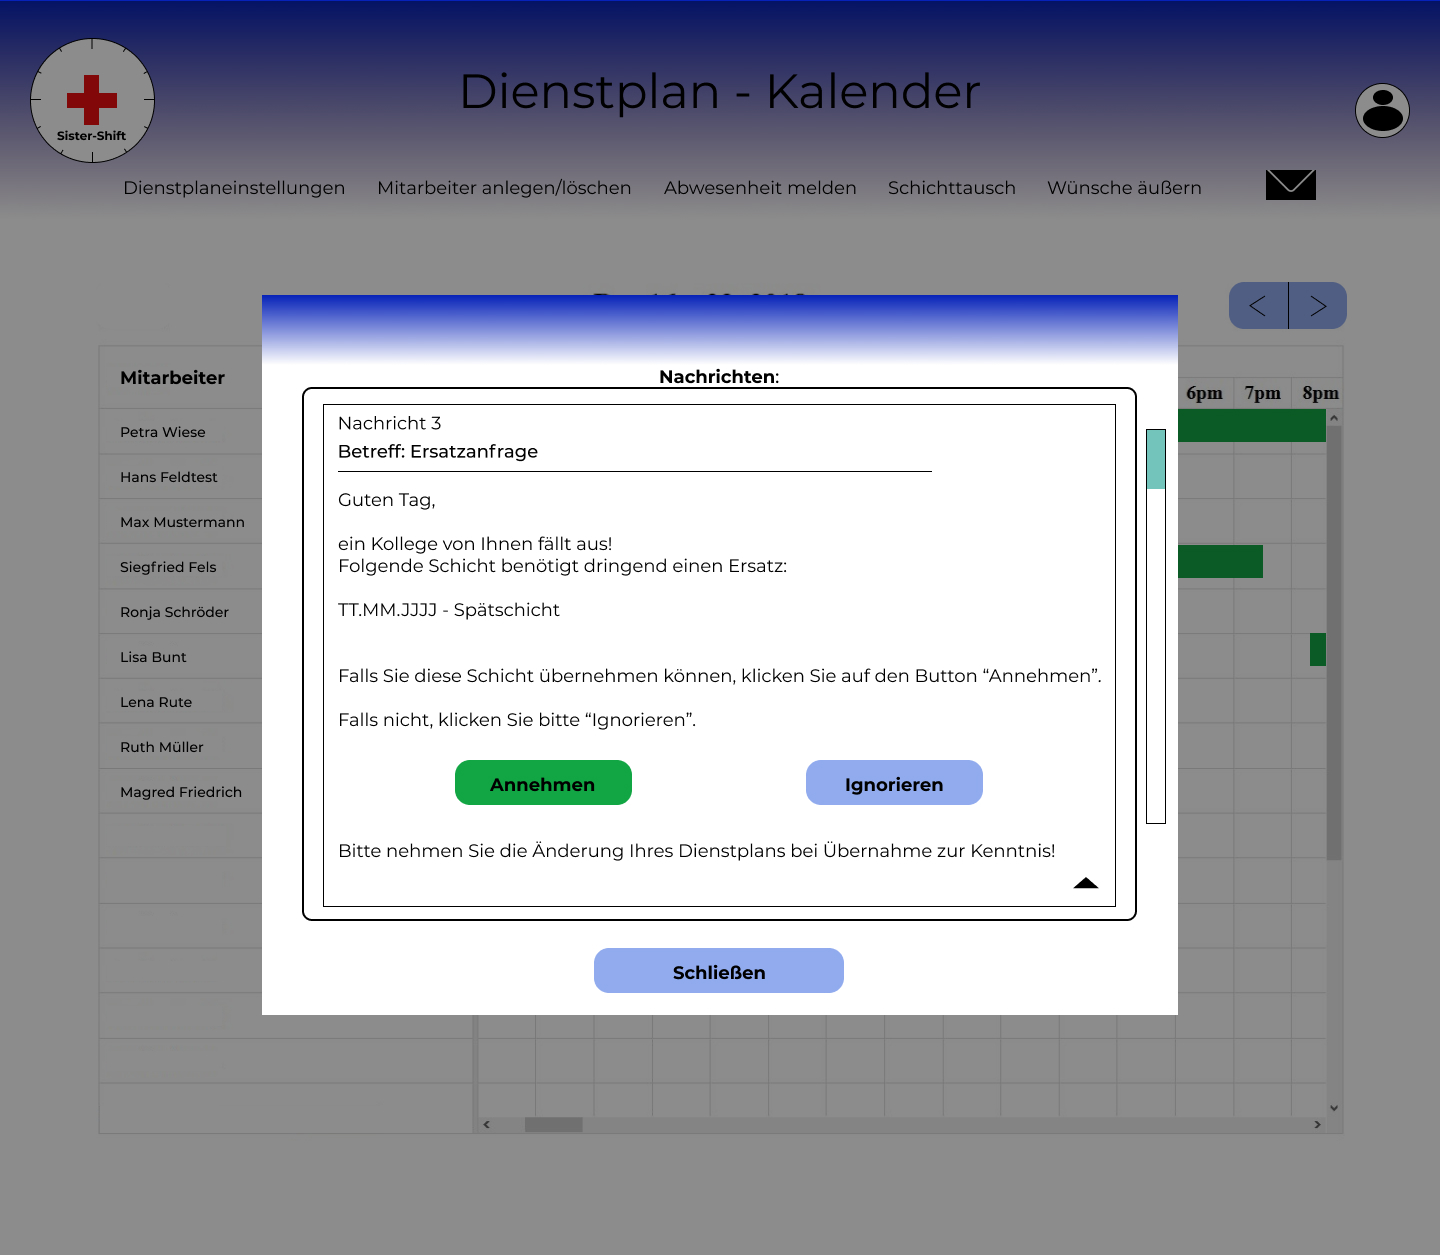
\includegraphics[width=1\textwidth]{Bilder/Screens/NachrichtErsatzanfrageangenommen.jpg}{\centering}
\caption{Nachricht Ersatzanfrage Angenommen}
\end{figure}
\begin{figure}[H]
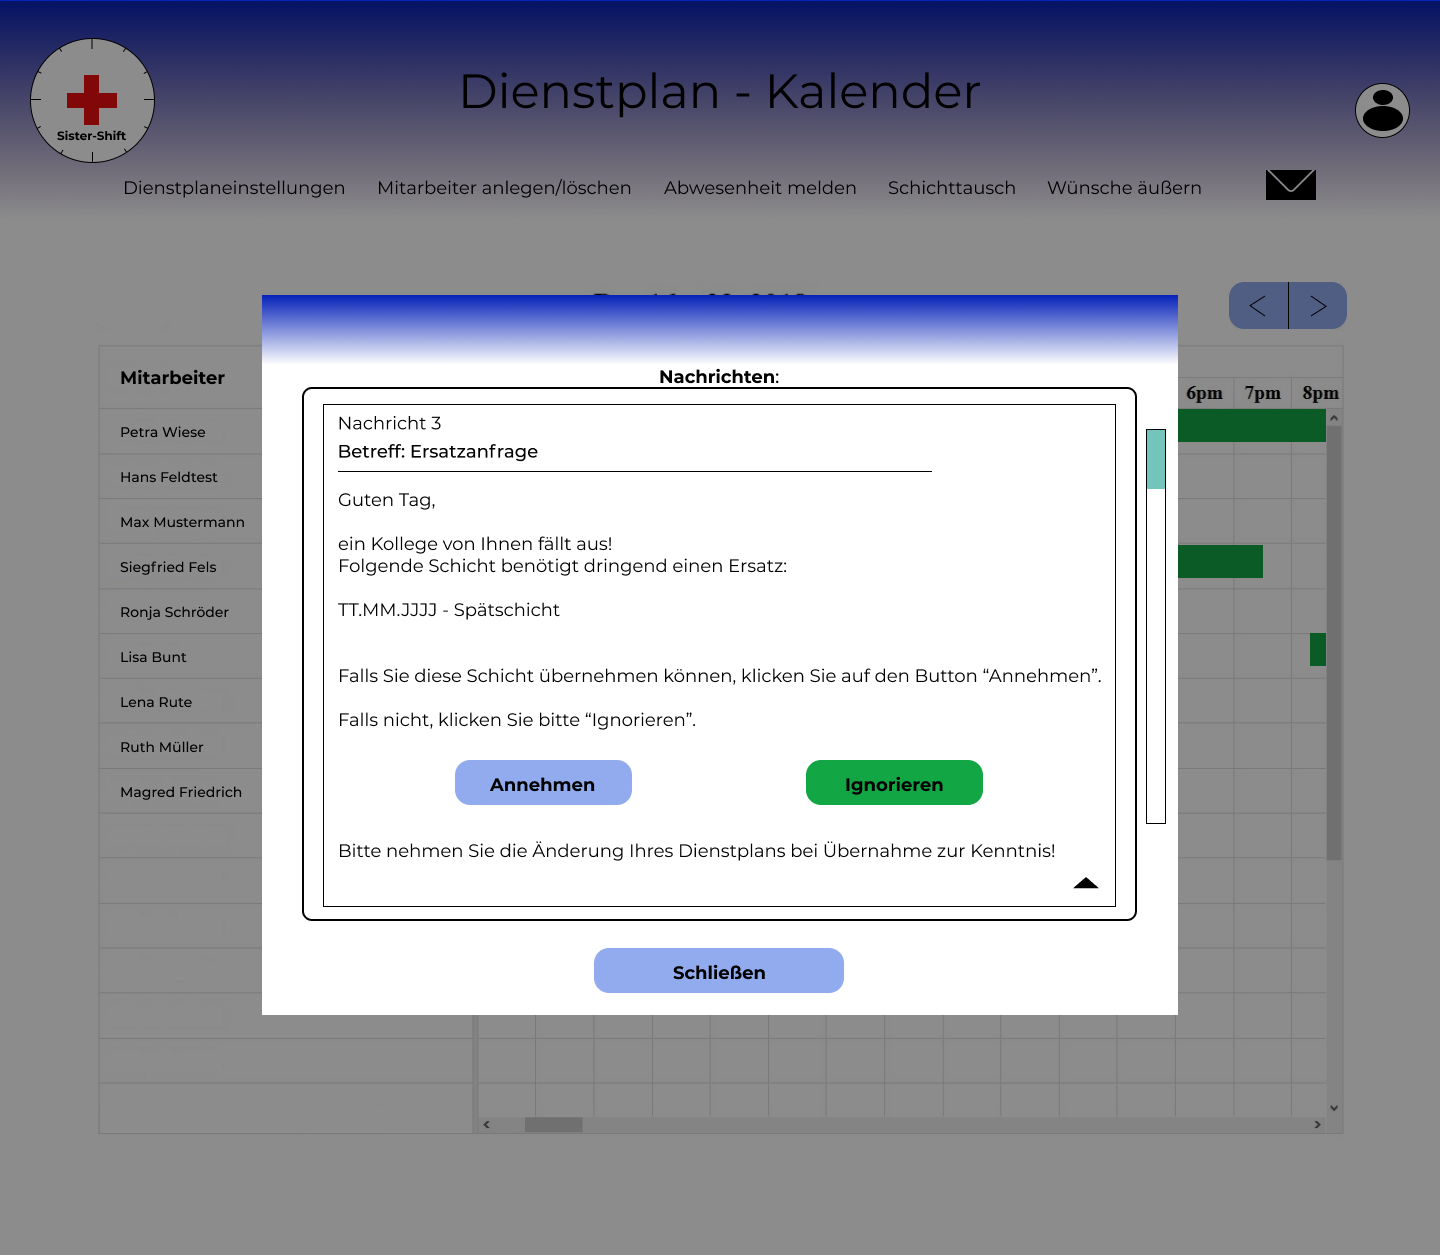
\includegraphics[width=1\textwidth]{Bilder/Screens/NachrichtErsatzanfrageabgelehnt.jpg}{\centering}
\caption{Nachricht Ersatzanfrage Abgelehnt}
\end{figure}
Die Benachrichtigungen eines Benutzers mit der Rolle Stationsleitung unterscheiden sich von den oben gezeigten Nachrichten. Es folgen die Nachrichten der Stationsleitung.
\begin{figure}[H]
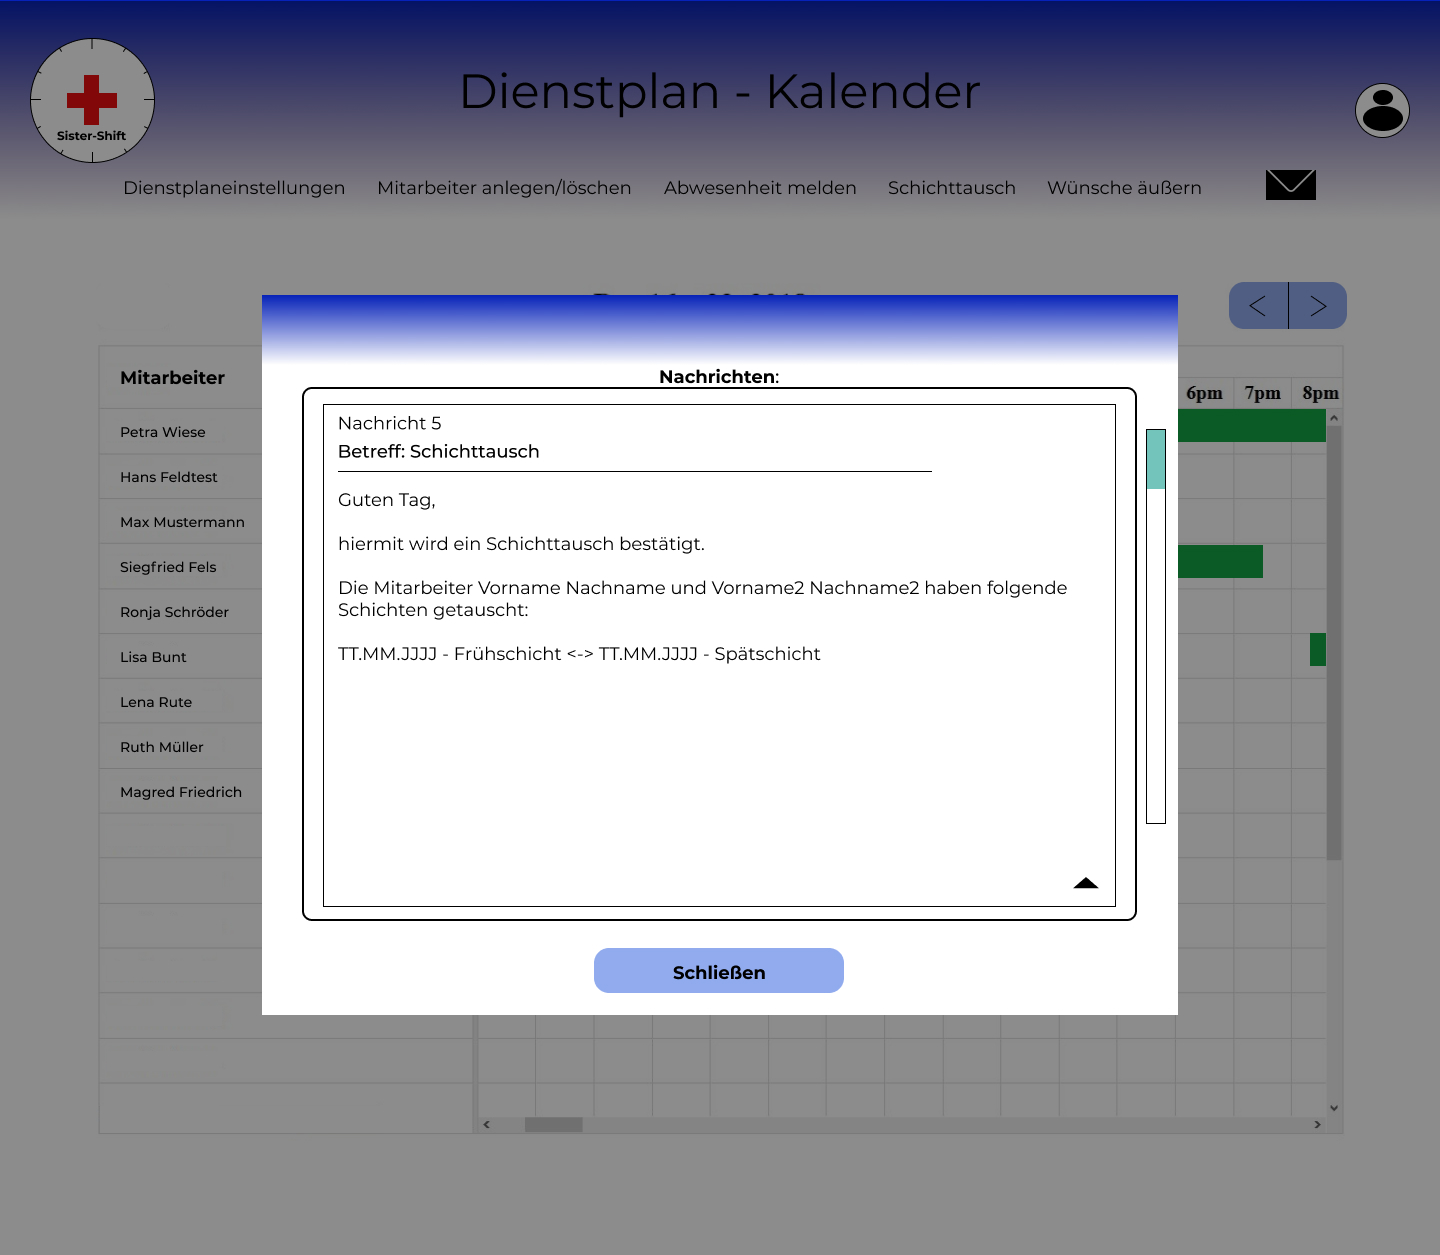
\includegraphics[width=1\textwidth]{Bilder/Screens/NachrichtStatleitungSchichttausch.jpg}{\centering}
\caption{Nachricht Schichttauschnotifikation}
\end{figure}
\begin{figure}[H]
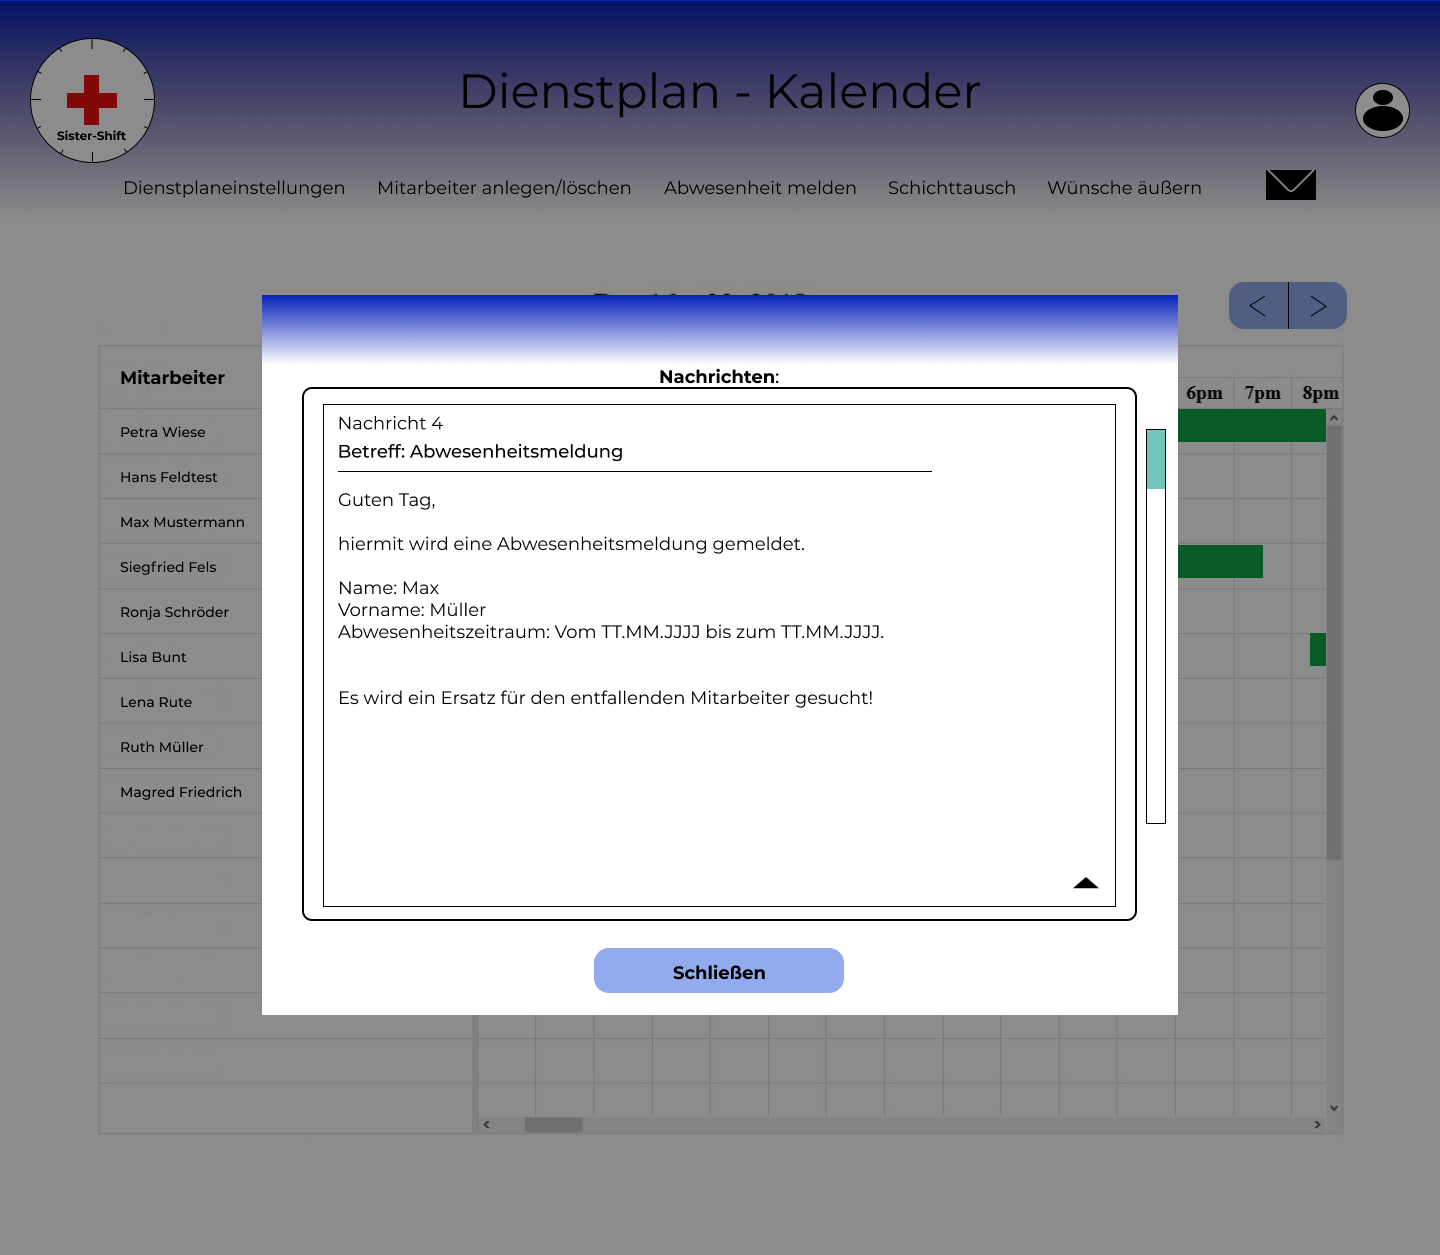
\includegraphics[width=1\textwidth]{Bilder/Screens/NachrichtStatleitungAbwesenheit.jpg}{\centering}
\caption{Nachricht Abwesenheitsnotifikation}
\end{figure}
\begin{figure}[H]
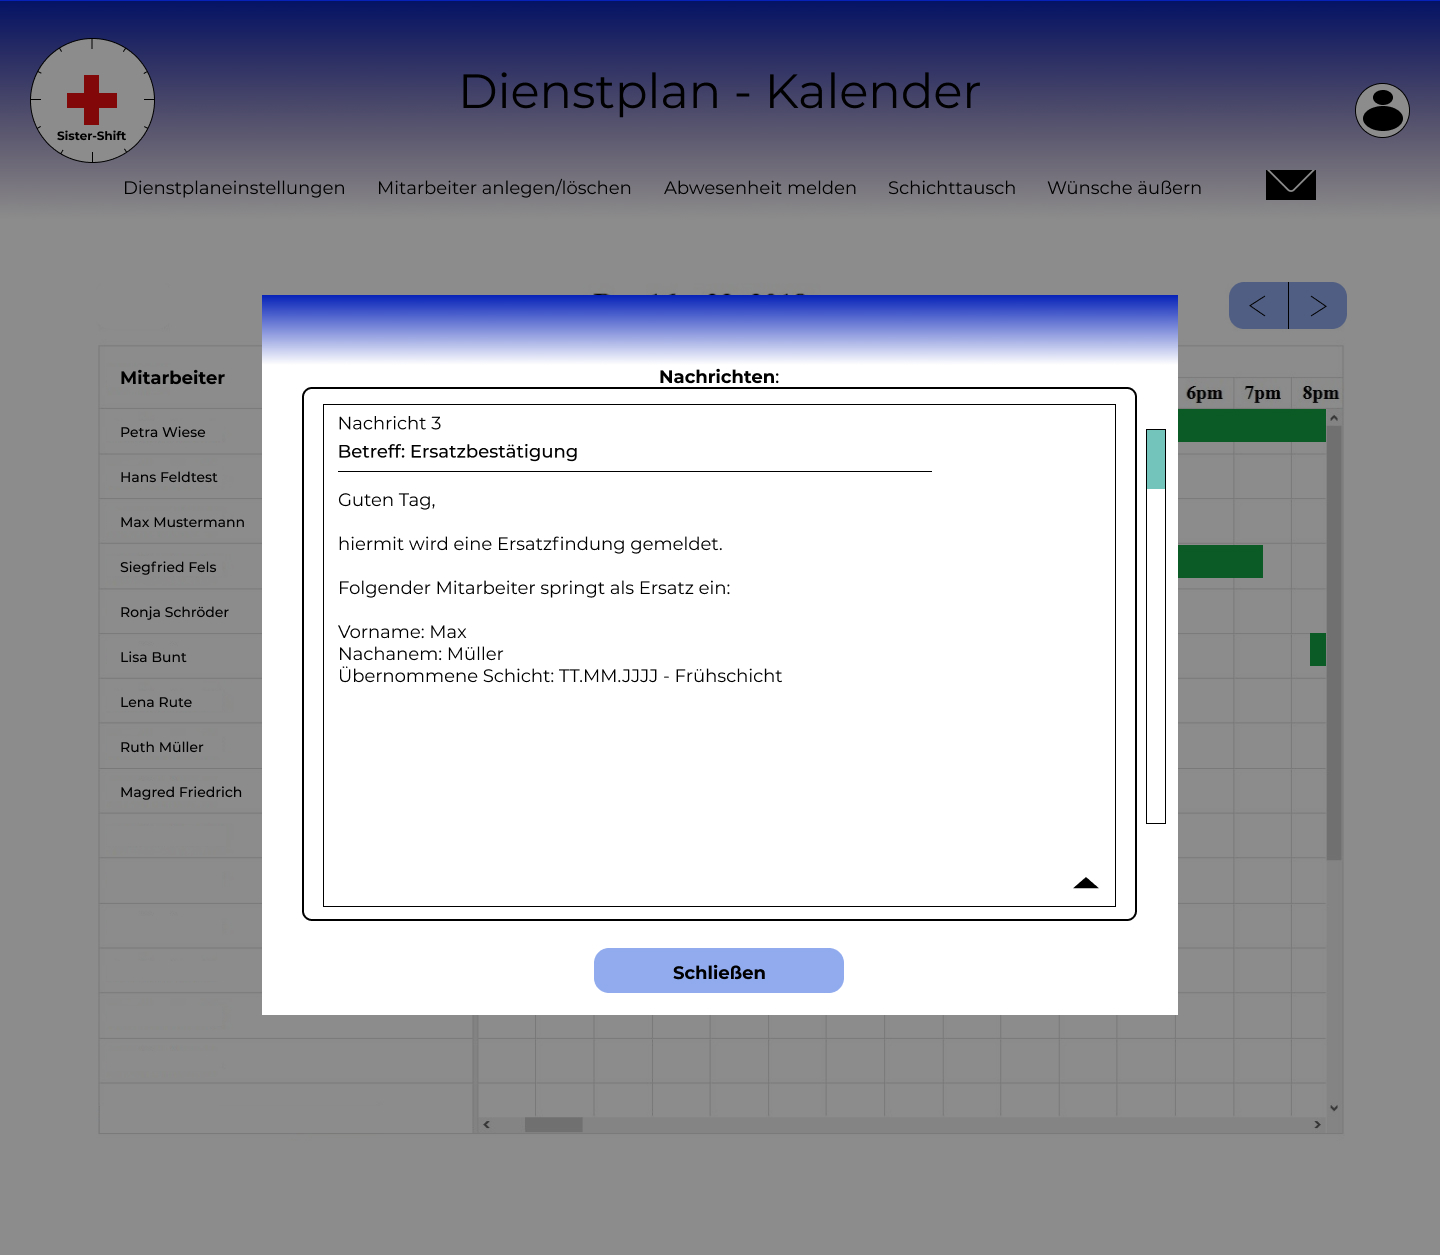
\includegraphics[width=1\textwidth]{Bilder/Screens/NachrichtStatleitungErsatzbestaetigung.jpg}{\centering}
\caption{Nachricht Ersatzbestätigung}
\end{figure}
\begin{figure}[H]
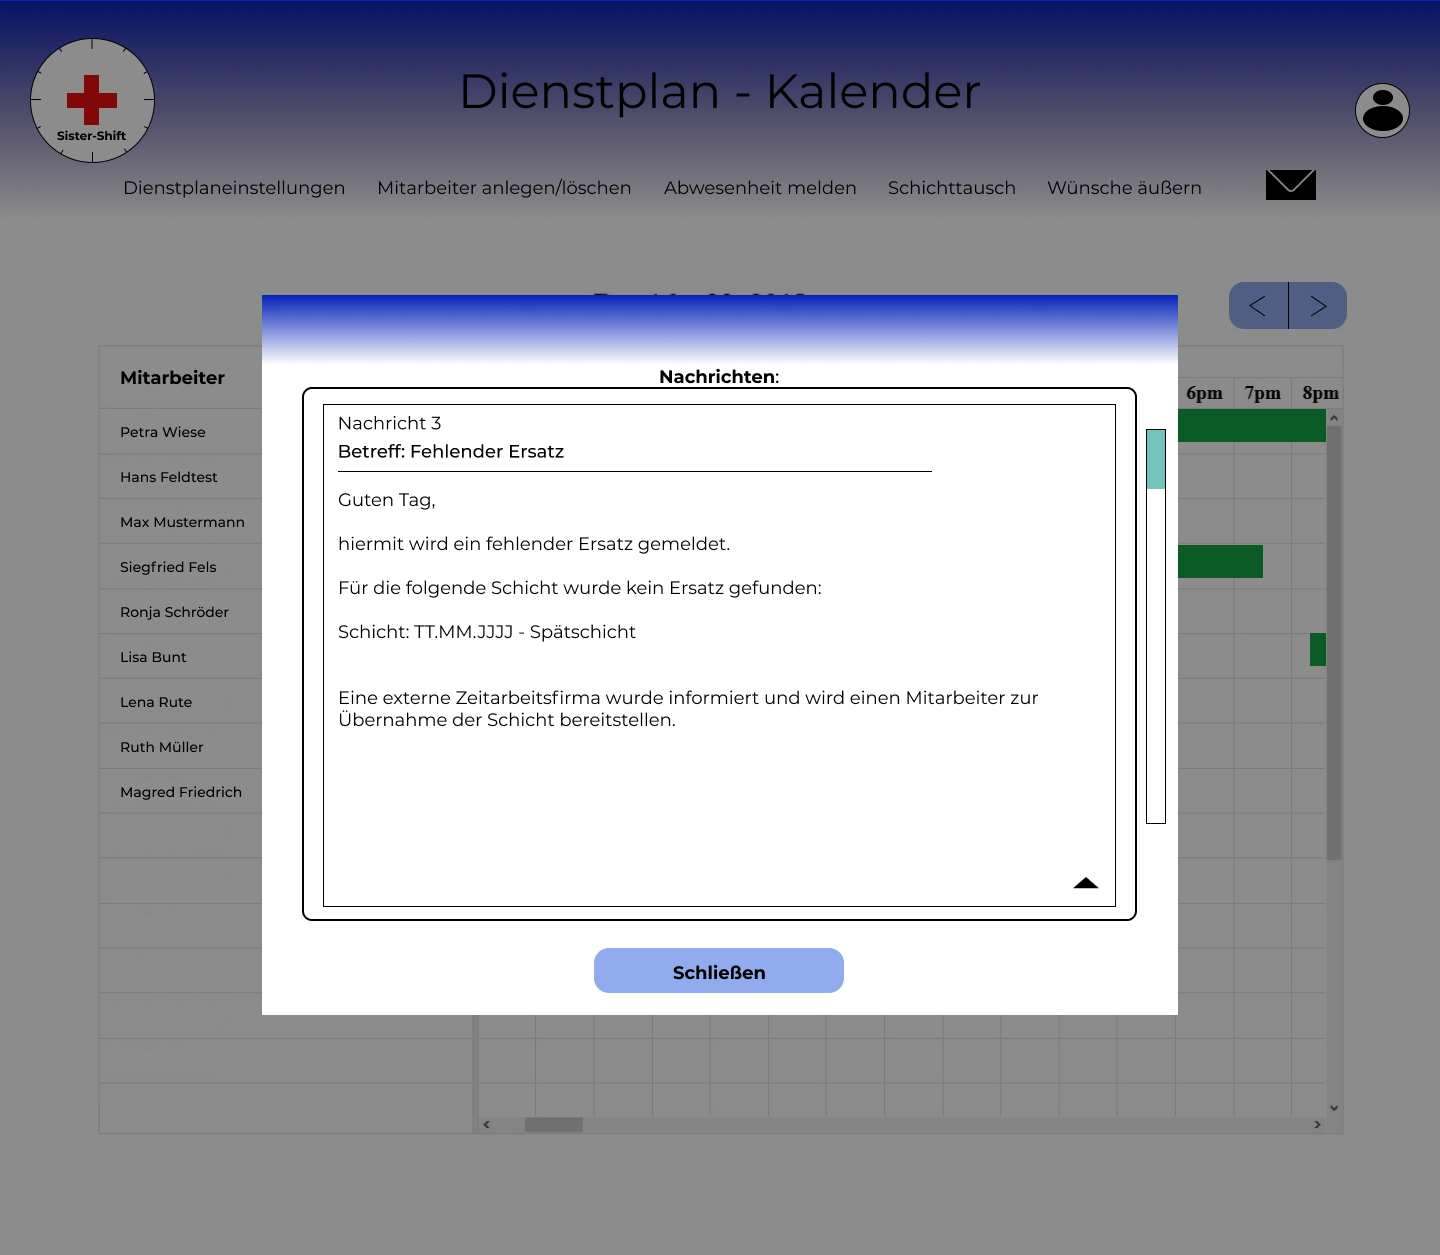
\includegraphics[width=1\textwidth]{Bilder/Screens/NachrichtStatleitungFehlenderErsatz.jpg}{\centering}
\caption{Nachricht fehlender Ersatz}
\end{figure}
\subsection{Dienstplaneinstellungen}
Zu sehen ist der Screen, auf welchem die Stationsleitung einen Dienstplan generieren kann. Bei erfolgreichem Generieren oder beim Misserfolg auf Grund fehlender Angaben erfolgt das Feedback über Dialogboxen.
\begin{figure}[H]
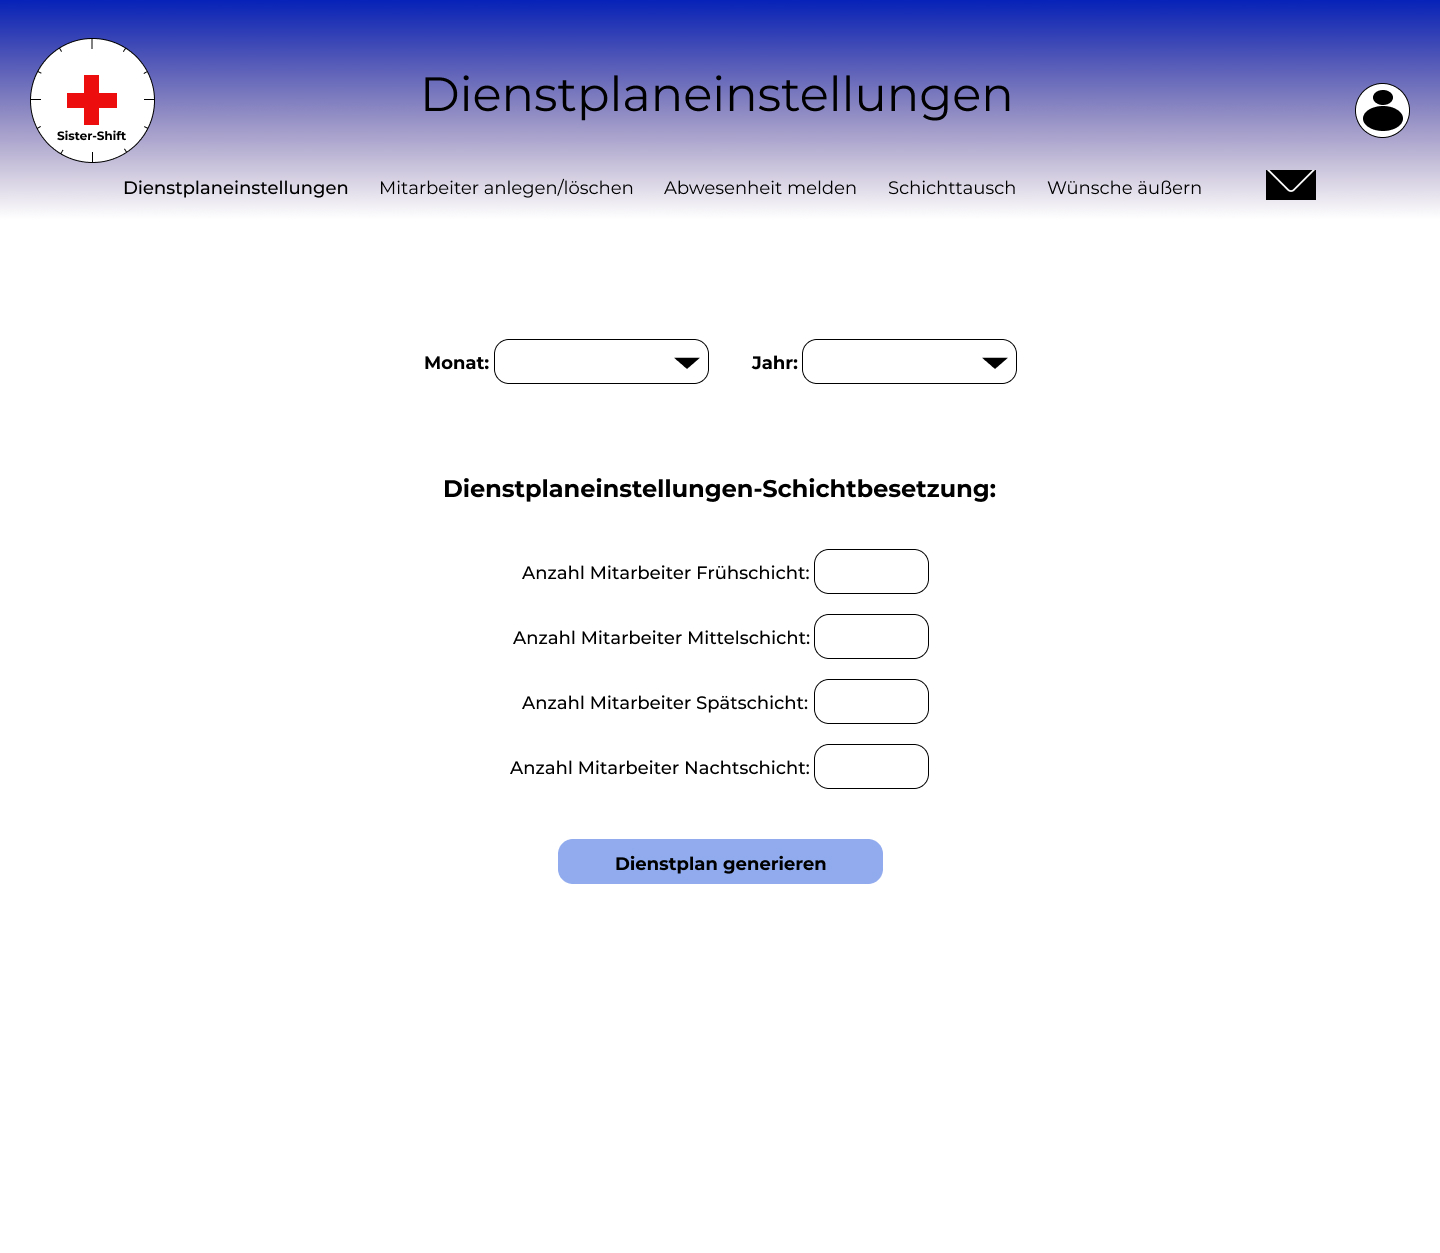
\includegraphics[width=1\textwidth]{Bilder/Screens/Dienstplaneinstellungen.jpg}{\centering}
\caption{Dienstplaneinstellungen}
\end{figure}
\begin{figure}[H]
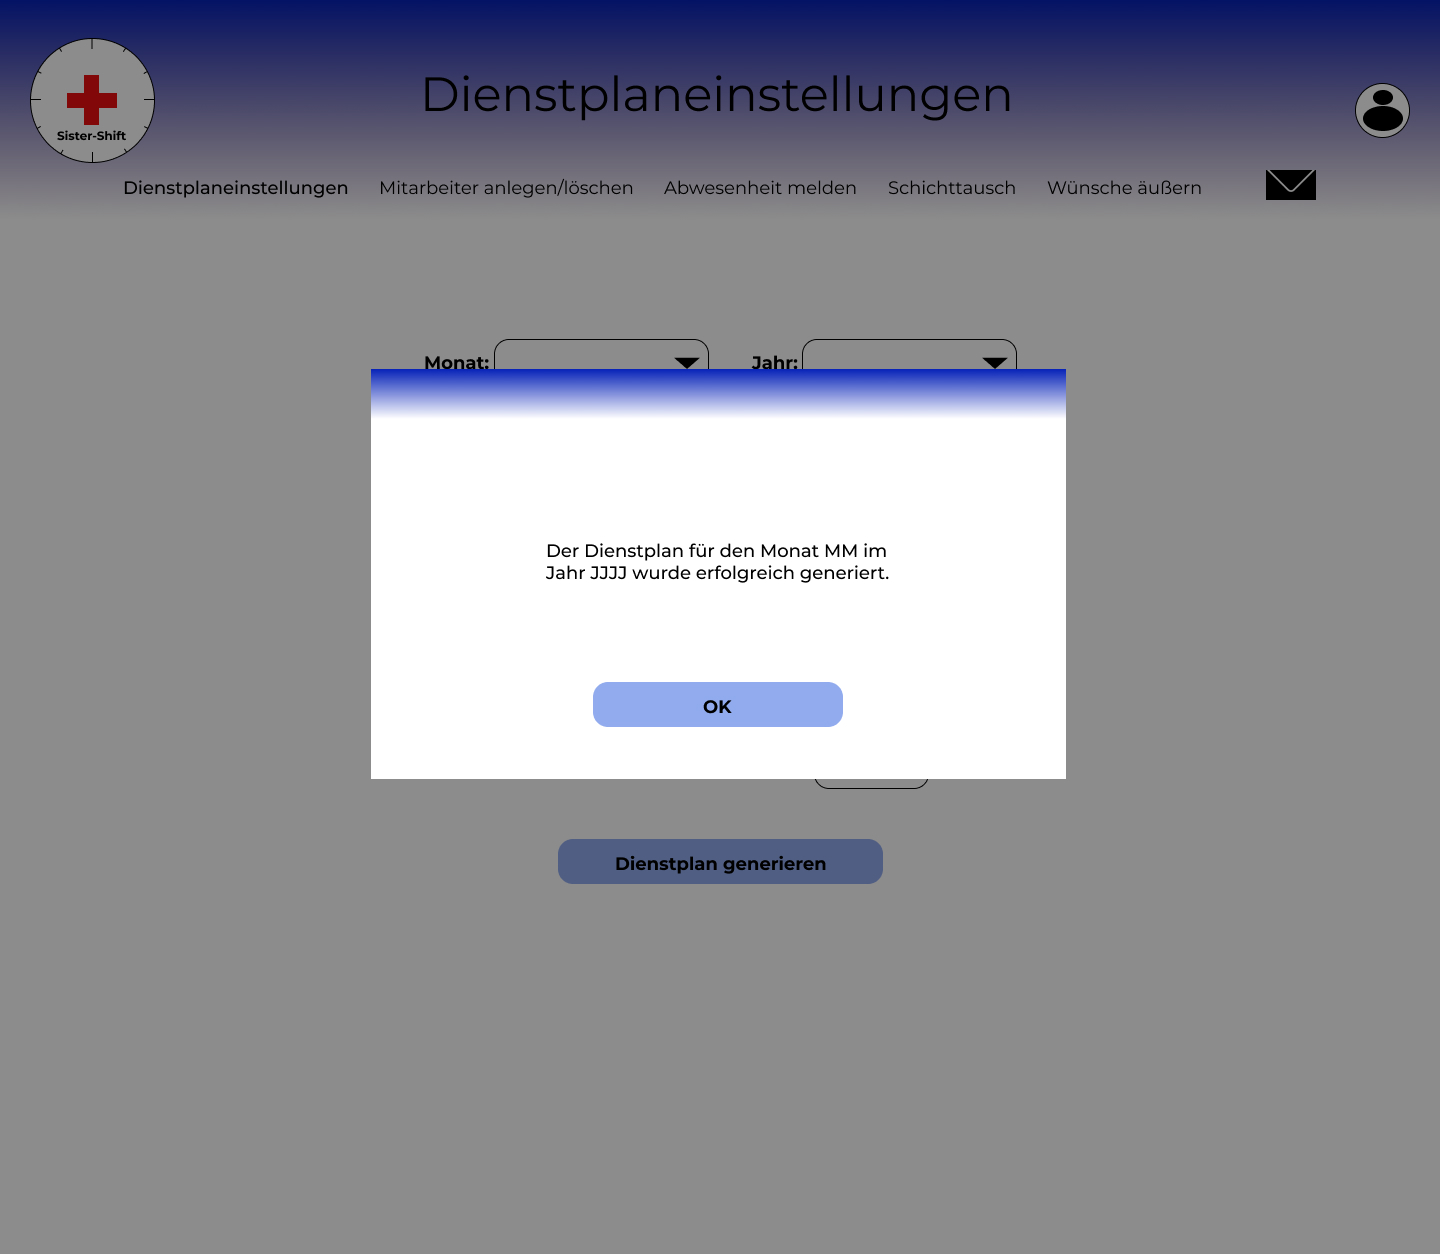
\includegraphics[width=1\textwidth]{Bilder/Screens/Dienstplaneinstellungen-Dialogbox.jpg}{\centering}
\caption{Dialogbox erfolgreiches Generieren}
\end{figure}
\begin{figure}[H]
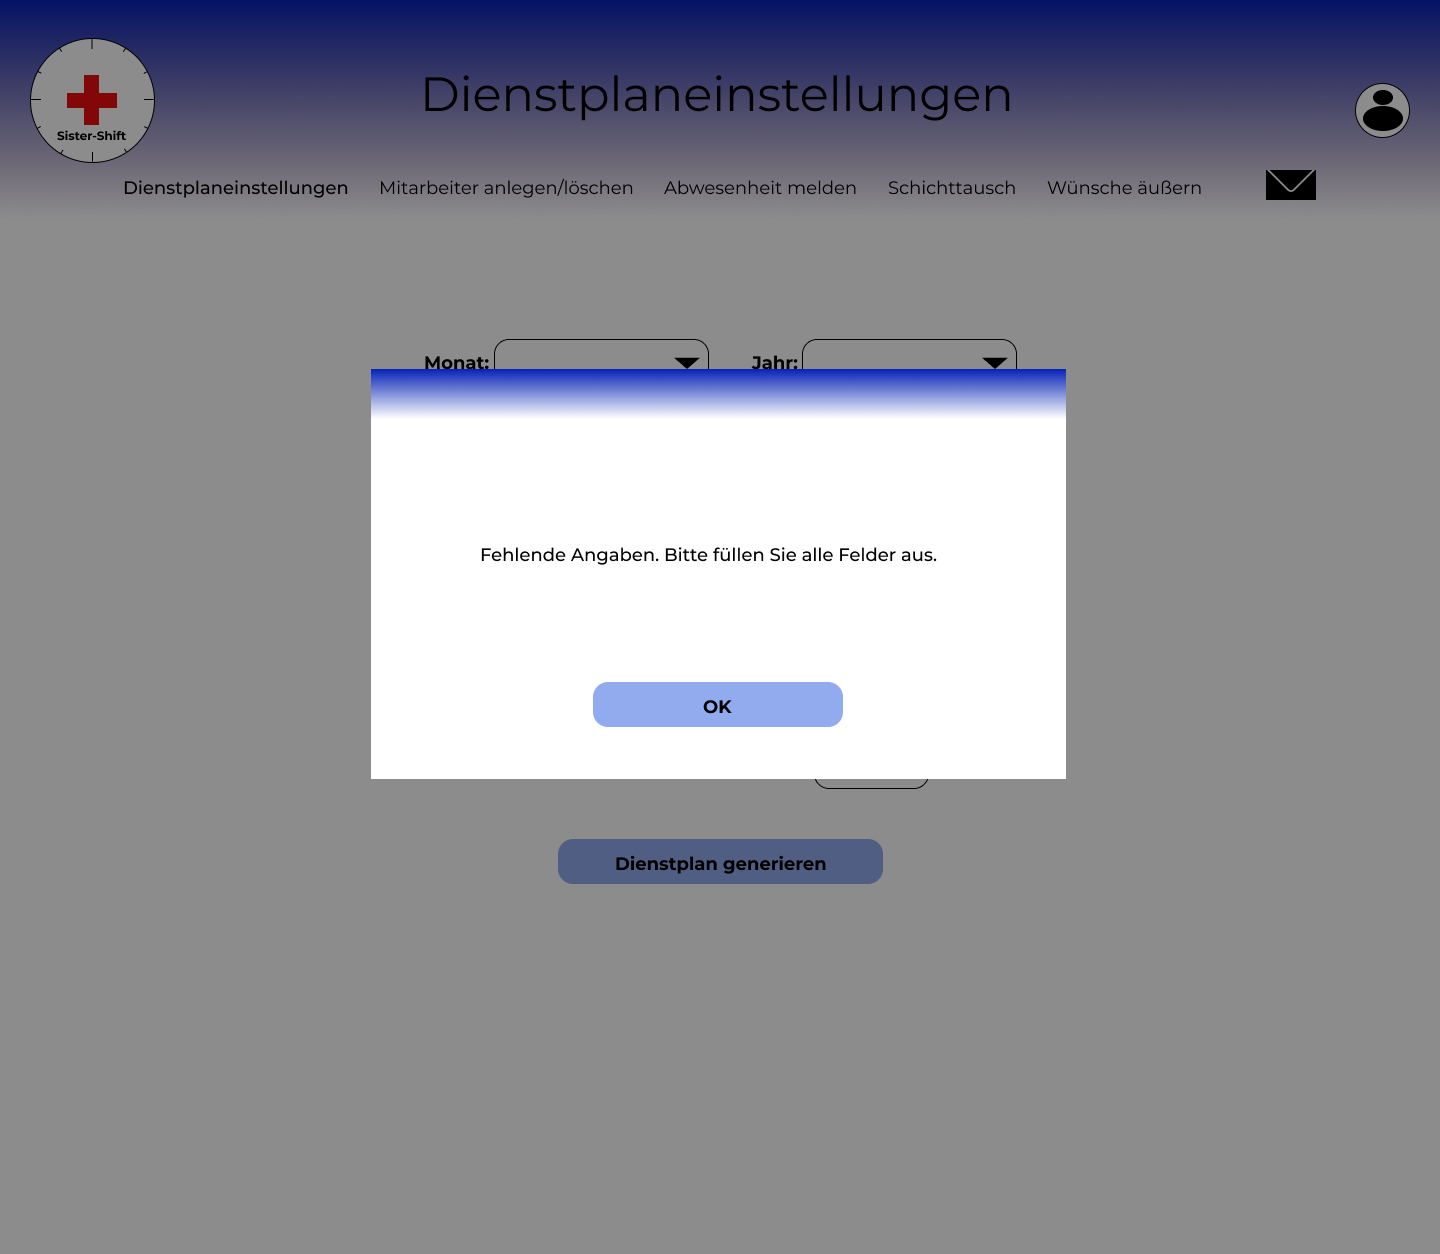
\includegraphics[width=1\textwidth]{Bilder/Screens/Dienstplaneinstellungen-Dialogbox(2).jpg}{\centering}
\caption{Dialogbox fehlende Angaben}
\end{figure}
Auf diesem Screen wird beispielhaft für alle Dropdown-Menüs der Anwendung die Gestaltung dieses gezeigt. Dies betrifft auch die Gestaltung der Interaktionsfläche, welche unter dem User-Icon zu finden ist.
\begin{figure}[H]
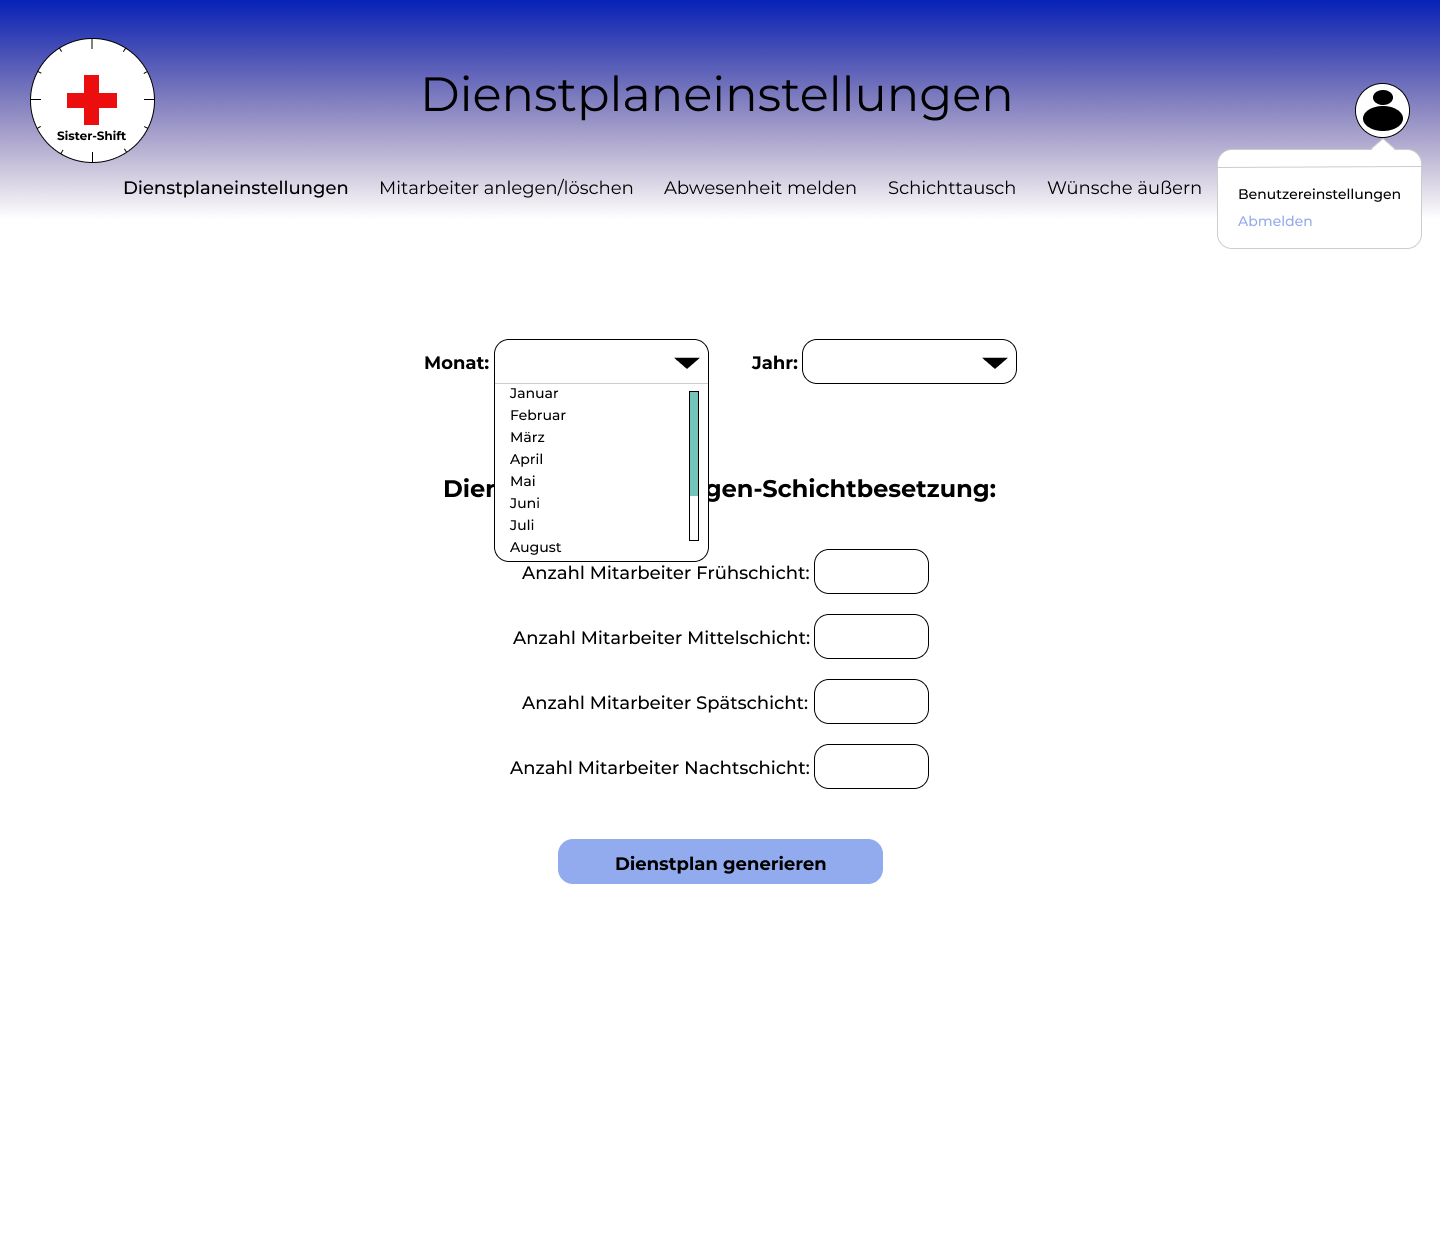
\includegraphics[width=1\textwidth]{Bilder/Screens/DropdownundUsersettings.jpg}{\centering}
\caption{Dropdown User Icon}
\end{figure}
\subsection{Benutzereinstellungen}
Durch Klicken auf den Unterpunkt Benutzereinstellungen unter dem Menü des User-Icons gelangt der Nutzer auf den Screen der Benutzereinstellungen. Hier können diverse Daten angepasst werden.
\begin{figure}[H]
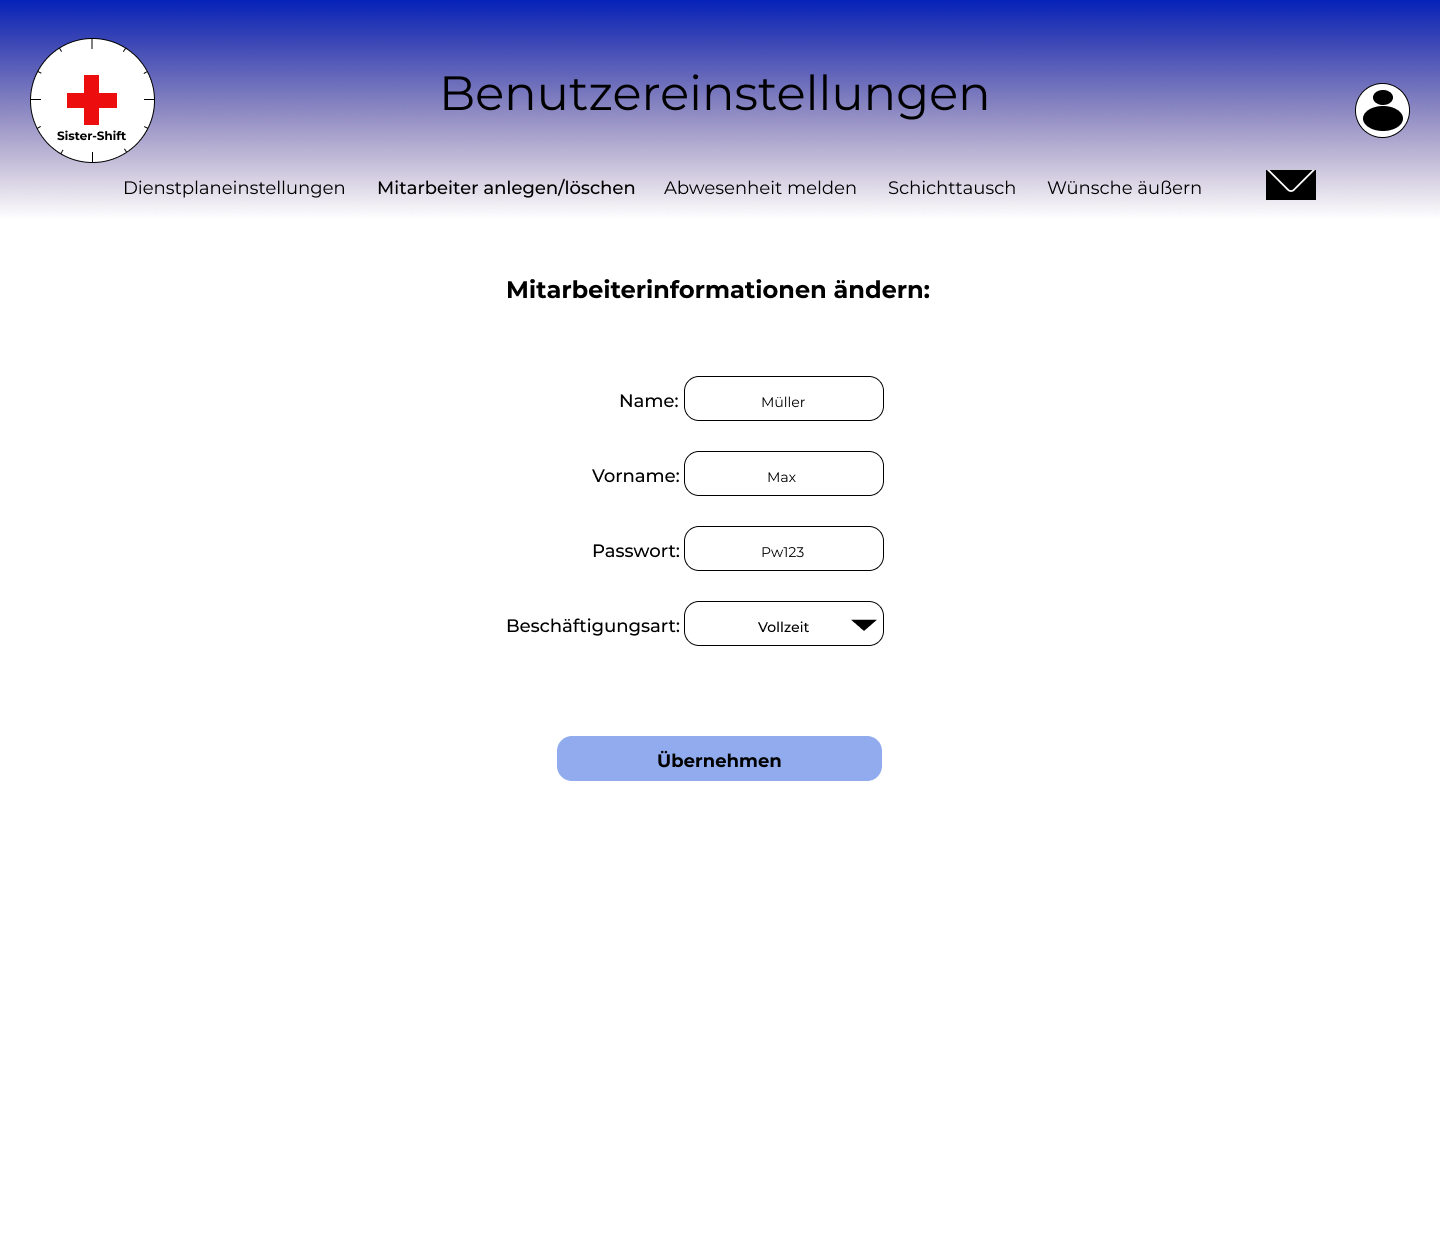
\includegraphics[width=1\textwidth]{Bilder/Screens/Benutzereinstellungen.jpg}{\centering}
\caption{Benutzereinstellungen}
\end{figure}
\begin{figure}[H]
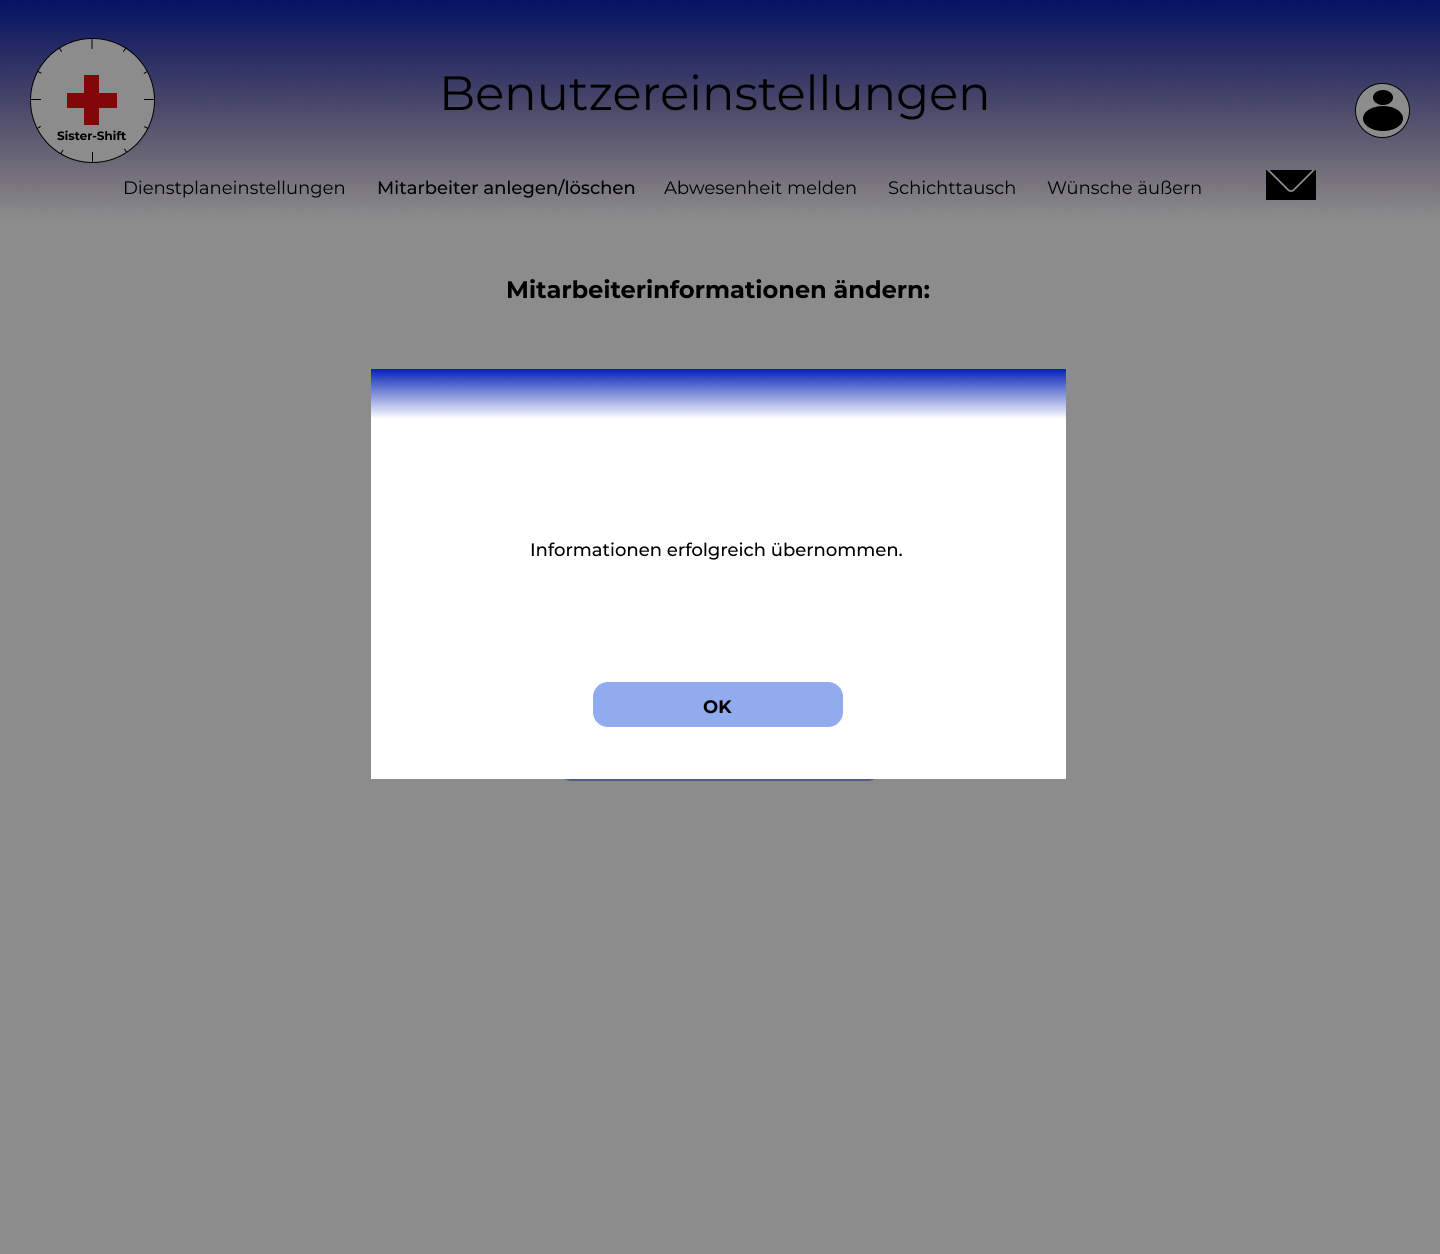
\includegraphics[width=1\textwidth]{Bilder/Screens/Benutzereinstellungen(1).jpg}{\centering}
\caption{Benutzereinstellungen - Dialogbox Erfolg}
\end{figure}
\begin{figure}[H]
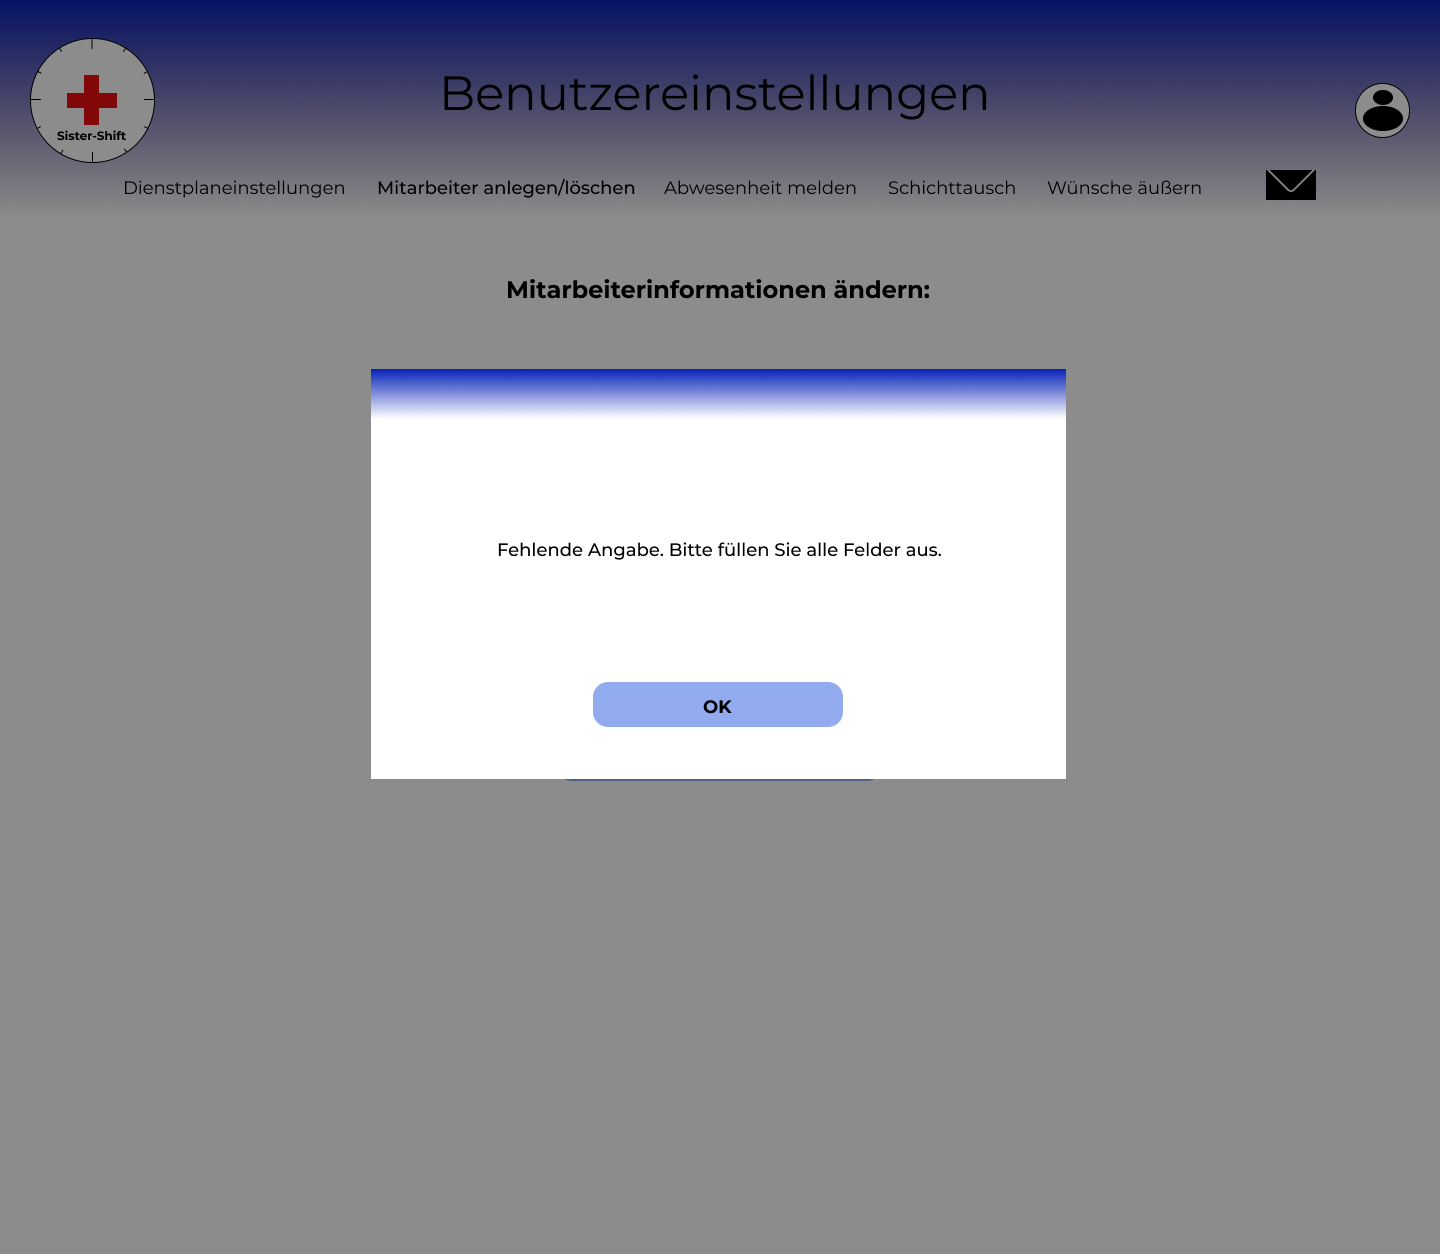
\includegraphics[width=1\textwidth]{Bilder/Screens/Benutzereinstellungen(2).jpg}{\centering}
\caption{Benutzereinstellungen Dialogbox Fehler}
\end{figure}
\subsection{Mitarbeiter anlegen/löschen}
Auf diesem Screen kann die Stationsleitung neue Mitarbeiter im System hinterlegen und bei Bedarf auch Mitarbeiter aus dem System entfernen.
\begin{figure}[H]
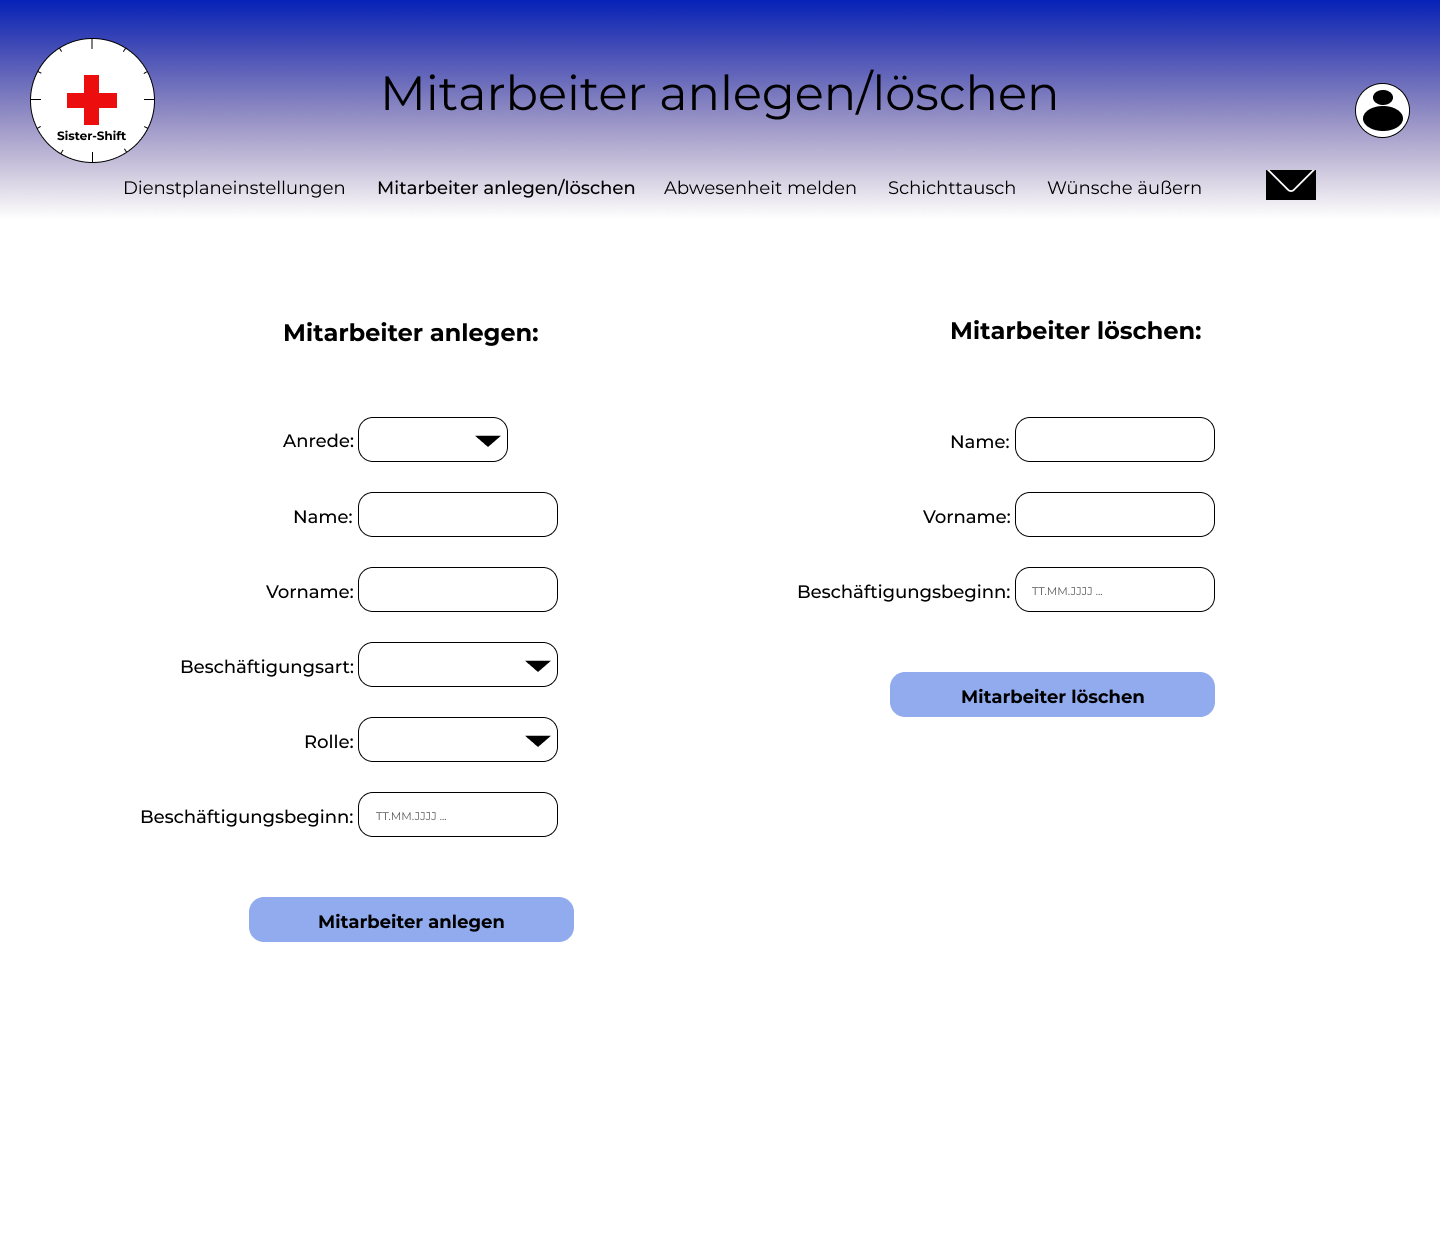
\includegraphics[width=1\textwidth]{Bilder/Screens/MAanlegen_Loeschen.jpg}{\centering}
\caption{Mitarbeiter anlegen/löschen}
\end{figure}
\begin{figure}[H]
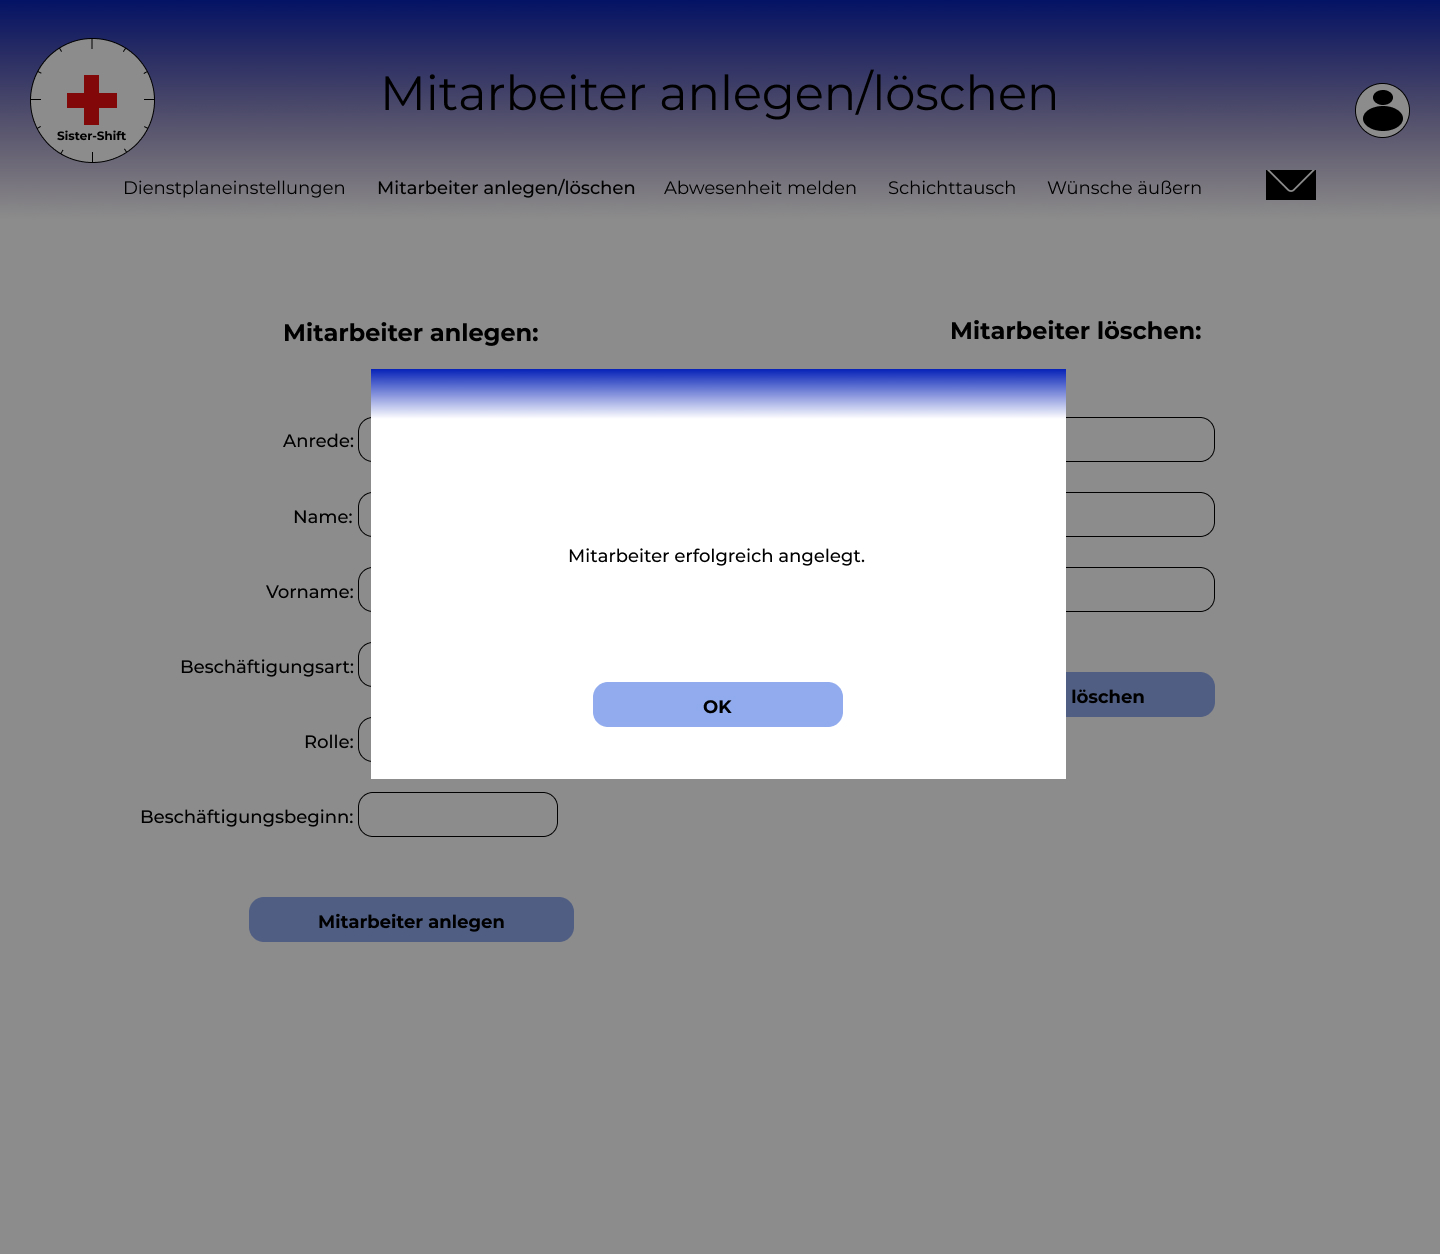
\includegraphics[width=1\textwidth]{Bilder/Screens/loeschen-Dialogbox(1).jpg}{\centering}
\caption{Dialogbox Erfolg Anlegen}
\end{figure}
\begin{figure}[H]
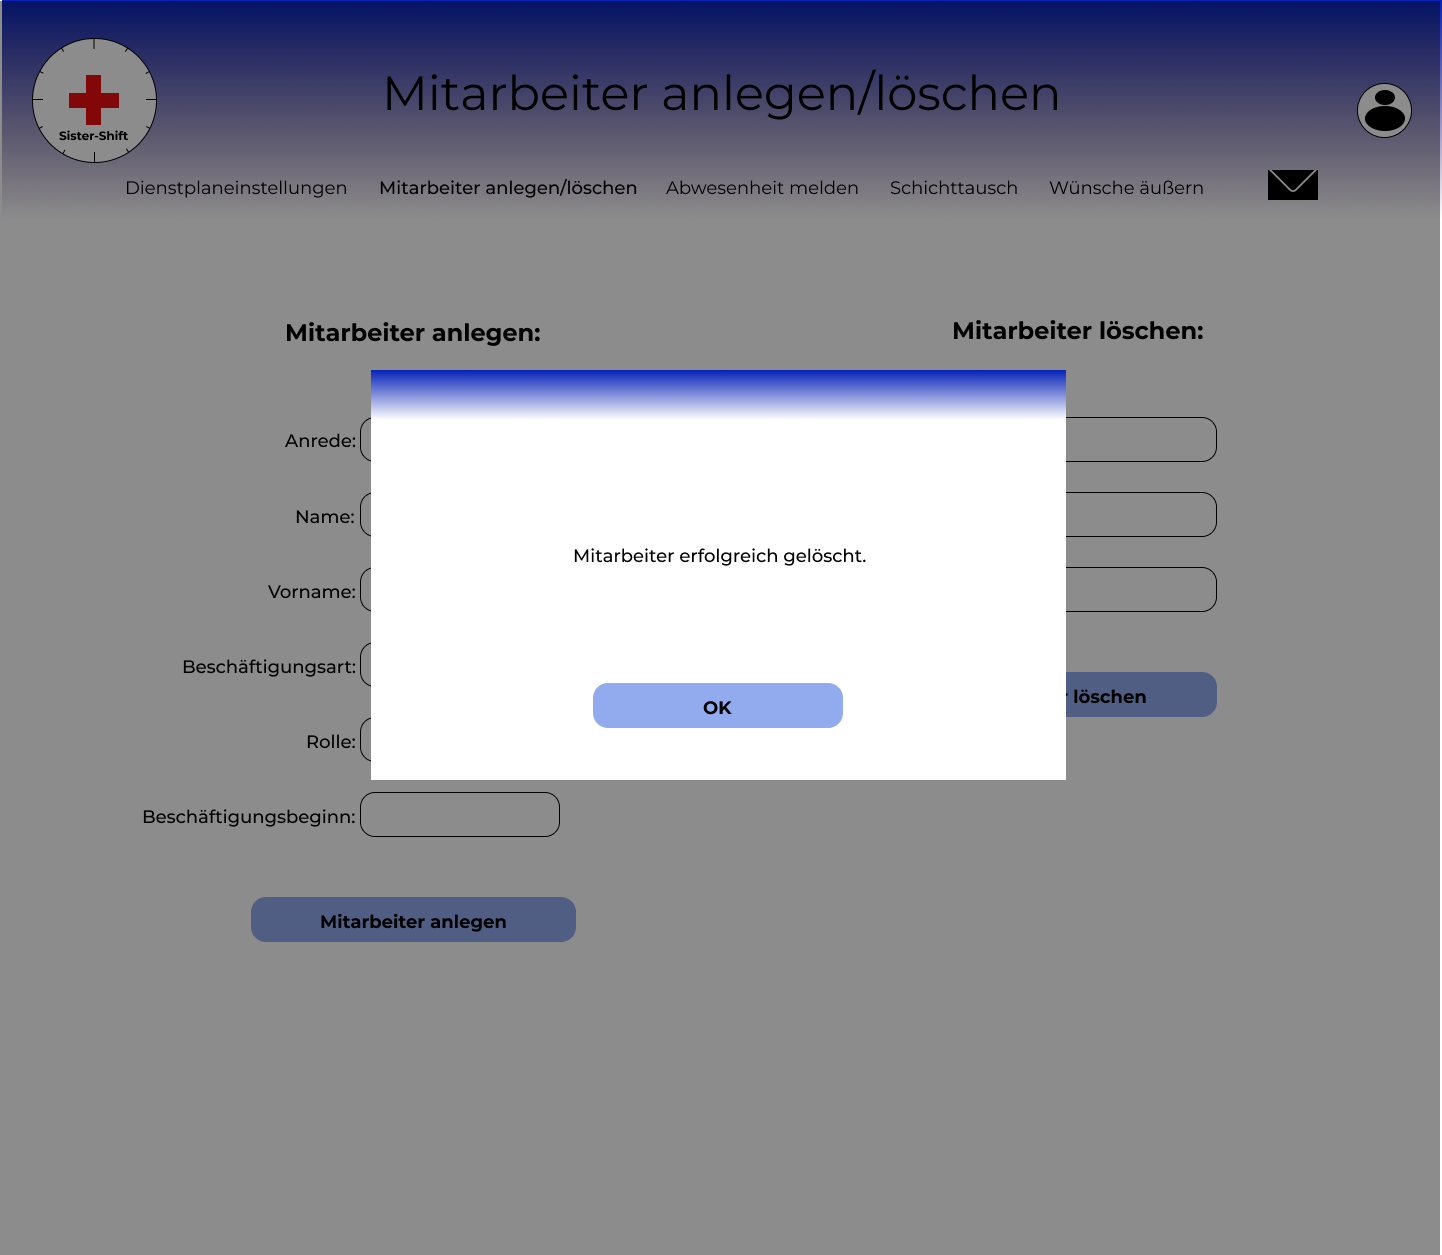
\includegraphics[width=1\textwidth]{Bilder/Screens/loeschen-Dialogbox(2).jpg}{\centering}
\caption{Dialogbox Erfolg Mitarbeiter löschen}
\end{figure}
\begin{figure}[H]
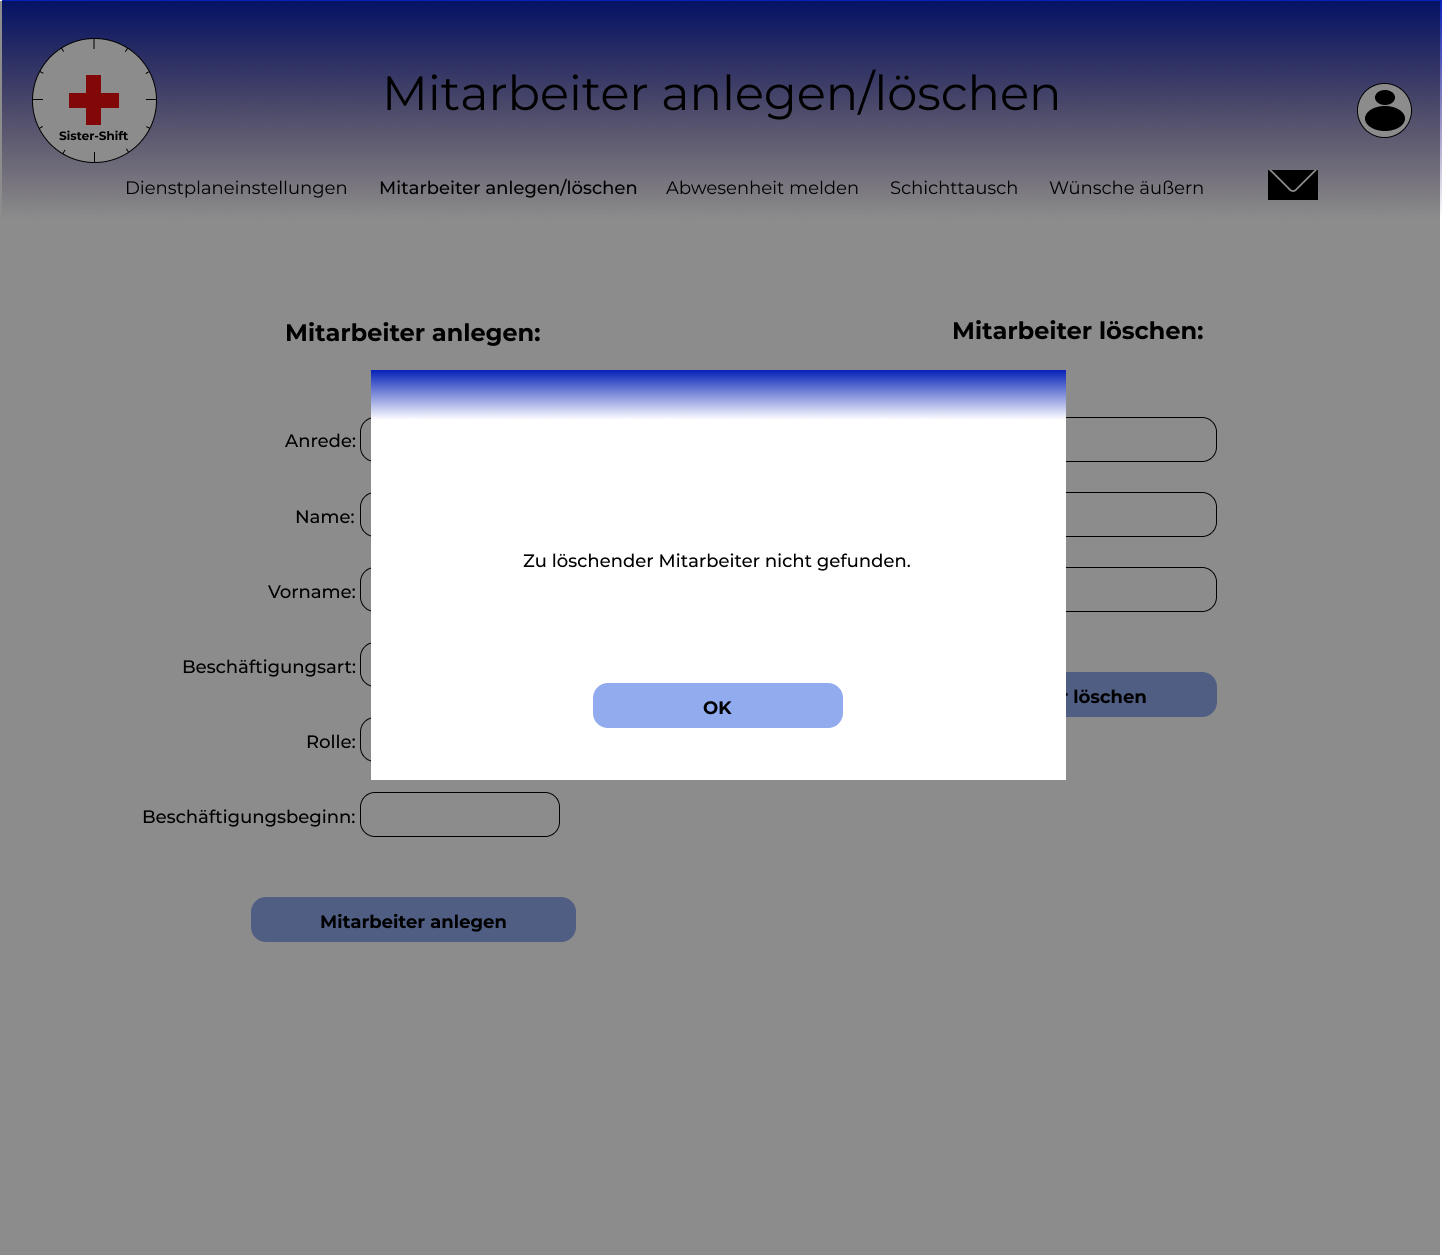
\includegraphics[width=1\textwidth]{Bilder/Screens/loeschen-Dialogbox(3).jpg}{\centering}
\caption{Dialogbox Misserfolg löschen}
\end{figure}
\begin{figure}[H]
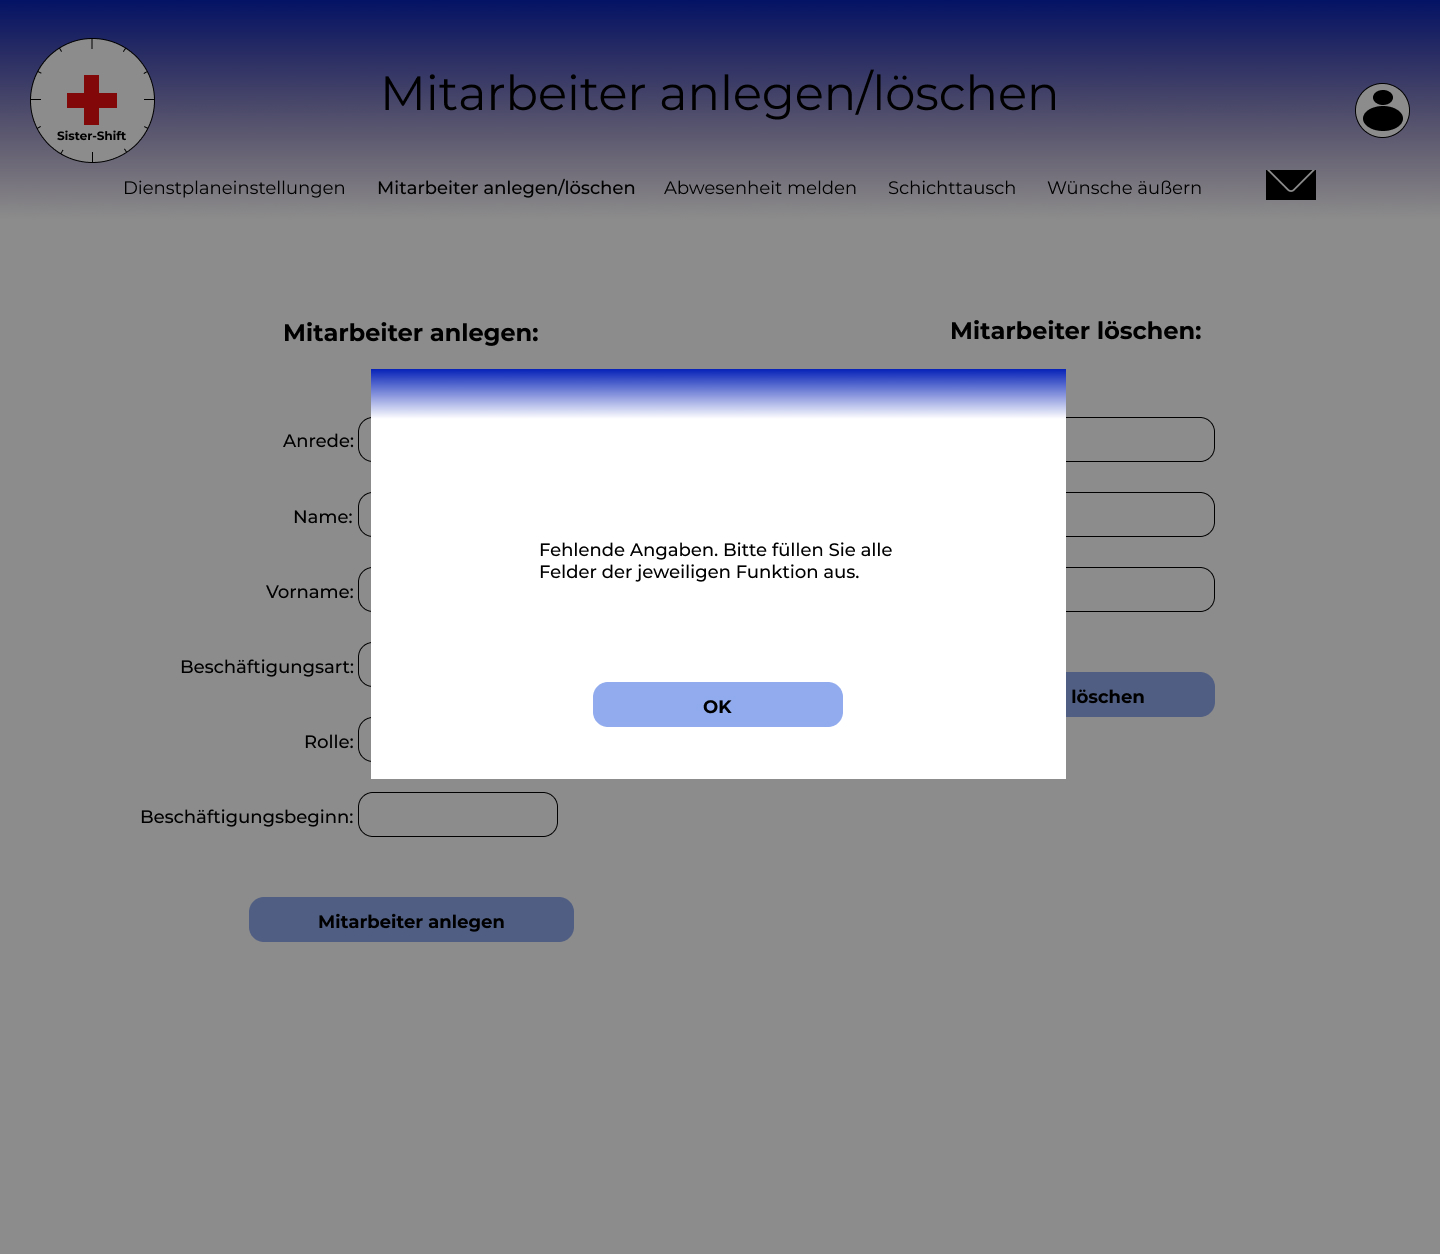
\includegraphics[width=1\textwidth]{Bilder/Screens/loeschen-Dialogbox(1)-1.jpg}{\centering}
\caption{Dialogbox Fehlende Angaben}
\end{figure}
\subsection{Abwesenheit melden}
Auf diesem Screen können sich die Krankenpfleger und Medizinischen Fachangestellten für einen Zeitraum abwesend melden und bei Bedarf einen Anhang und Kommentar mit an diese Meldung hängen.
Durch Klicken auf Abwesenheit melden, öffnet sich ein Dialogfenster, in dem eine Interaktion vom Nutzer erzwungen wird. Er wird aufgefordert die Eingabe zu kontrollieren und die Abwesenheit anschließend zu bestätigen. Wird diese Bestätigt, erhält der Nutzer eine Nachricht als Bestätigung für das Melden der Abwesenheit.
\begin{figure}[H]
\includegraphics[width=1\textwidth]{Bilder/Screens/Abwesenheitmelden.jpg}{\centering}
\caption{Abwesenheit melden}
\end{figure}
Durch Klicken auf Abwesenheit melden, öffnet sich ein Dialogfenster, in dem eine Interaktion vom Nutzer erzwungen wird. Er wird aufgefordert die Eingabe zu kontrollieren und die Abwesenheit anschließend zu bestätigen. Wird diese Bestätigt, erhält der Nutzer eine Nachricht als Bestätigung für das Melden der Abwesenheit.
\begin{figure}[H]
\includegraphics[width=1\textwidth]{Bilder/Screens/Abwesenheitmelden-1.jpg}{\centering}
\caption{Dialogbox Überprüfung}
\end{figure}
\begin{figure}[H]
\includegraphics[width=1\textwidth]{Bilder/Screens/Abwesenheitmelden-2.jpg}{\centering}
\caption{Dialogbox fehlende Angaben}
\end{figure}
\subsection{Schichttausch}
Zu sehen ist der Screen, auf dem ein Schichttausch angefragt werden kann. Der User gibt das Datum an, an dem die Schicht liegt, die dieser gerne tauschen würde. Ist der Tausch erfolgreich, wird die Schicht entfernt, und der jeweilige User bekommt eine neue Schicht über eine Benachrichtigung zugewiesen. Diese Information ist für den User auch nochmal nachzulesen. 
\begin{figure}[H]
\includegraphics[width=1\textwidth]{Bilder/Screens/Schichttausch.jpg}{\centering}
\caption{Schichttausch}
\end{figure}
\begin{figure}[H]
\includegraphics[width=1\textwidth]{Bilder/Screens/Schichttausch-1.jpg}{\centering}
\caption{Dialogbox Schichttausch Erfolg}
\end{figure}
\begin{figure}[H]
\includegraphics[width=1\textwidth]{Bilder/Screens/Schichttausch-2.jpg}{\centering}
\caption{Dialogbox Schichttausch fehlende Angaben}
\end{figure}
\subsection{Wunschäußerung}
Auf diesem Screen können die Mitarbeiter Wünsche zum Dienstplan äußern. Dabei geben diese ein Datum an, auf das nach Möglichkeit keine Schicht gelegt wird. Falls dies nicht umsetzbar ist, können die Mitarbeiter eine Schicht priorisieren, welche an dem Datum am passendsten wäre. Diese Informationen sind ebenfalls auf dem Screen nachzulesen.
\begin{figure}[H]
\includegraphics[width=1\textwidth]{Bilder/Screens/Wunschaeusserung.jpg}{\centering}
\caption{Wunschäußerung}
\end{figure}
\begin{figure}[H]
\includegraphics[width=1\textwidth]{Bilder/Screens/Wunschaeusserung-1.jpg}{\centering}
\caption{Dialogbox Wunschäußerung Erfolg}
\end{figure}
\begin{figure}[H]
\includegraphics[width=1\textwidth]{Bilder/Screens/Wunschaeusserung-2.jpg}{\centering}
\caption{Dialogbox Wunschäußerung fehlende Angaben}
\end{figure}
\section{Evaluation}
Im Usability Engineering Lifecycle nach Deborah J. Mayhew gibt es 3 Phasen der Evaluation. Zunächst gibt es die Iterative Conceptual Model Evaluation [vgl. Deborah J. Mayhew: The Usability Engineering Lifecycle, S.229], darauf folgt die Iterative Screen Design Standards Evaluation [vgl. Deborah J. Mayhew: The Usability Engineering Lifecycle, S.297] und schlussendlich erfolgt die Iterative Detailed User Interface Design Evaluation [Deborah J. Mayhew: The Usability Engineering Lifecycle, S.339]. Da das Projekt zeitlich sehr begrenzt ist, können die Phasen nicht alle durchlaufen werden. In diesem Projekt wird nur eine Evaluation nach der Erstellung des Detailed User Interface durchgeführt. Es wird also das Interface aus dem Kapitel Detailed User Interface evaluiert. Dabei wird die Methode des Cognitive Walkthrough gewählt, welche von Professor Dr. Hartmann an der TH Köln Campus Gummersbach im Modul Mensch-Computer-Interaktion gelehrt wurde. 
\subsection{Benutzer}
Die Benutzer des Systems sind bereits im Kapitel User-Profiles ermittelt und beschrieben worden.
\subsection{Szenarien}
Um einen Cognitive Walkthrough durchführen zu können müssen realistische und dem späteren Einsatz des Systems entsprechende Szenarien konstruiert und abgearbeitet werden. Es werden für die User Stationsleitung und Krankenpfleger Szenarien beschrieben. Medizinische Fachangestellte fallen in diesem Fall unter das Szenario der Krankenpfleger.\\\\

1. Stationsleitung: Die Stationsleitung soll einen Dienstplan für einen beliebigen Monat generieren.\\\\
2. Stationsleitung: Die Stationsleitung soll einen neuen Mitarbeiter im System anlegen.\\\\
3. Krankenpfleger: Ein Krankenpfleger soll seinen Dienstplan einsehen. \\\\
4 Krankenpfleger: Ein Krankenpfleger soll eine Abwesenheit melden. \\\\
5 Krankenpfleger: Ein Krankenpfleger soll die ungelesenen Nachrichten lesen und falls nötig beantworten.\\\\
\subsection{Handlungen zu den Szenarien}
Szenario 1: \\\\
Die Stationsleitung loggt sich in das System ein. Danach klickt diese auf den Menüpunkt Dienstplaneinstellungen in der Navigationsleiste. Auf dem entsprechenden Screen füllt diese die erforderten Eckdaten aus und klickt auf den Button “Dienstplan generieren”. Sofern alle Eingaben gemacht wurden, bestätigt die Stationsleitung nur noch das Feedback zur erfolgreichen Generierung eines Dienstplans.\\\\
Szenario 2: \\\\
Die Stationsleitung loggt sich in das System ein. Danach klickt diese auf den Menüpunkt Mitarbeiter anlegen/löschen in der Navigationsleiste. Auf dem entsprechenden Screen füllt diese die erforderten Eckdaten aus und klickt auf den Button “Mitarbeiter anlegen”. Sofern alle Eingaben gemacht wurden, bestätigt die Stationsleitung nur noch das Feedback der erfolgreichen Aktion.\\\\
Szenario 3:\\\\
Der Krankenpfleger loggt sich in das System ein. Danach landet jeder User auf dem Hauptscreen der Dienstplan – Kalender – Ansicht. Auf diesem muss der Krankenpfleger nur noch seinen Namen suchen und kann seine Schichten einsehen. Falls eine weiter Woche eingesehen werden möchte, klickt der Krankenplfeger auf den entsprechenden Button um die Woche auf dem Kalender zu wechseln.\\\\
Szenario 4:\\\\
Der Krankenpfleger loggt sich in das System ein. Danach klickt dieser auf den Menüpunkt Abwesenheit melden in der Navigationsleiste. Auf dem entsprechenden Screen füllt diese die erforderten Eckdaten aus (Abwesenheitszeitraum) und klickt auf den Button “Abwesenheit melden”. Sofern alle Eingaben gemacht wurden, bestätigt der Krankenpfleger nur noch das Feedback der erfolgreichen Aktion. Optional können durch einen “Anhang”- Button auch Dokumente mitgeschickt werden und nach Bedarf ein Kommentar zur Meldung verfasst werden. \\\\
Szenario 5:\\\\
Der Krankenpfleger loggt sich in das System ein. Um Nachrichten einzusehen, klickt dieser auf das Briefsymbol in der Navigationsleiste. Nach dem Öffnen einer Dialogbox kann der Krankenpfleger alle Benachrichtigungen einsehen. Durch Klicken auf eine, kann dieser eine Nachricht im Detail lesen und bei Bedarf direkt beantworten.
\subsection{Fazit des Cognitive Walkthrough}
Die Evaluation mit einer Krankenschwester der Notaufnahme des Klinikum Leverkusen hat gezeigt, dass die entworfenen Szenarien bereits bei der erstmaligen Benutzung des Systems erfolgreich absolviert wurden. Dieses Ergebnis ist der leichten, strukturierten und übersichtlichen Gestaltung des Interfaces zu verdanken. Zudem sind die Usereingaben kurz und das System erfordert allgemein nur sehr wenig Input eines Users. Ein Faktor, der ebenfalls zur Lernförderlichkeit beiträgt, sind kleine Informationstexte an Inputfeldern, welche etwaige Fragen des Users im Vorhinein klären. \\\\
Da die Stationsleitung nicht für eine Evaluation bereitstehen , wurden die 2 Szenarien dieser ebenfalls von einer Krankenschwester durchgeführt. Auch bei diesen Szenarien gab es auf Grund der Einfachheit und dem minimalen Aufwand keine Probleme die Szenarien reibungslos und ohne Auftauchen von Fragen abzuarbeiten. 

\subsection{Fazit}
Insgesamt wären 3 Evaluationen erstrebenswert gewesen, um die Ergebnisse noch zu perfektionieren. Dies ist allerdings auf Grund des knappen Zeitrahmens nicht möglich gewesen. Die Evaluation dient dazu, den User mit in den Entwicklungsprozess einzubinden und etwaige Probleme, oder schlechte Umsetzungen zu identifizieren und in einer Iteration zu beseitigen.
Bei der Evaluation zum Interface tauchten keine Probleme oder Anmerkungen zur Verbesserung der Benutzeroberfläche auf, weshalb keine weiteren Iterationen nötig sind.
\section{Zielerreichung}
Nach der Erstellung des Detailed User Interface werden die im Kapitel Usability Goals genannten Ziele an das User Interface überprüft und ausgewertet.
\subsection{Einfaches,intutives,lernförderliches Design}
Die gewählten Farben im Styleguide suggerieren dem User eine gewissen Positivität und Einfachheit. Durch einen weißen Untergrund wirkt das Interface sehr aufgeräumt. Verschiedene Elemente sind zeitgemäß und überlagern sich nicht. Der User erhält nur Informationen, sofern dies nötig ist und wird nicht mit unnötigem Input belastet. Einem immer fest fixierte Menüleiste erleichtert das Navigieren. Durch die Umsetzung der Screen Design Standards wird der Nutzer schnell mit der Benutzung der Anwendung vertraut.
\subsection{Aussagekräftige, einfach verständliche Darstellungen der wichtigsten Informationen und Herausstellen von Benachrichtigungen}
Benachrichtigungen können in einer separaten Dialogbox übersichtlich und schnell eingesehen werden. Die Nachrichten des Systems selbst sind verständlich und kurz gehalten.  Hat ein Nutzer ungelesene Nachrichten, so wird dies durch eine Rote Zahl am Benachrichtigung-Icon deutlich gemacht. Der Dienstplan-Kalender ist gut lesbar, und die Sekundärfarbe des Styleguides hebt die Schichten deutlich vom weißen Untergrund ab. Zusatzinformationen zu Eingabefeldern sind verständlich formuliert und in schwarzer Farbe gehalten.
\subsection{Datenkosistenz}
Da alle Nutzer des Systems auf denselben Dienstplan zugreifen und angezeigt bekommen, ist eine Datenkonsistenz gegeben. Ändert sich z.B. die Schicht eines Krankenpflegers, so wird diese Aktualisierung bei jedem Nutzer zu sehen sein.
\subsection{Automatisierung der Verarbeitung von Tauschanfrage, Wunschäußerungen und Ersatzfindung}
Die jeweiligen Funktionen sind gut über die Navigationsleiste zu erreichen. Der Input zu diesen beschränkt sich auf 1-2 Usereingaben. Somit ist der Input, der vom Benutzer zu tätigen ist sehr gering. Die Eingabefelder sind verständlich benannt und bei Bedarf erhält der User einen Informationstext zu der jeweiligen Eingabe. Durch das einfache Design und dem Vorhandensein von nur einem Button wird dem User die Nutzung der jeweiligen Funktionen schnell klar. Der User erhält nach jedem Ausführen einer Aktion Feedback und das System übernimmt den Rest der jeweiligen Funktion.
\subsection{Benutzer zugeschnittene Interfaces}
Verschiedene Nutzer haben verschiedene Zugriffsrechte auf Funktionen. So beinhaltet das Interface für die Krankenpfleger und medizinischen Fachangestellten nicht die Ansichten für die Funktionen Dienstplaneinstellungen und Mitarbeiter anlegen/löschen. Diese Funktionen sind der Stationsleitung vorbehalten.
\section{Spezifikation der Dienstschnittstellen}
\subsection{Dienstgeber}
Der Dienstgeber stellt eine Schnittstelle nach dem defacto Standard REST dar.
Über diese Schnittstelle kann der Dienstnutzer den Dienstgeber ansprechen. Somit kann dieser den Service des Dienstgebers nutzen. Der Service umfasst das Erstellen von automatisierten Dienstplänen und das Finden von Ersatz bei Abwesenheiten. Beim Erstellen des Dienstplans müssen folgende Faktoren beachtet werden: Gesetzliche Rahmenbedingungen, Krankenhaus spezifische Rahmenbedingungen [vgl. Konzept Domänenrecherche], die Wünsche der Mitarbeiter, die faire Verteilung der Schichten (Aufteilung Feiertage, Wocheneden sowie Schichtenwechsel). Dies soll vom Dienstgeber allein beachtet werden. Bei der Ersatzfindung muss der Dienstgeber geeigneten Ersatz finden. Dies bedeutet, dass nach Eingang einer Abwesenheitsmeldung, nur Personal angefragt werden darf, das auf derselben Station arbeitet, das am Tag der Abwesenheit nicht arbeitet, dass trotz Einspringens 10 oder mehr Stunden Ruhepause hat und im Idealfall keine oder am wenigsten Überstunden hat. Wurde geeignetes Personal gefunden muss die Stationsleitung über den gesamten Vorgang informiert werden und der Dienstplan angepasst werden.
\subsection{Dienstnutzer}
Der Dienstnutzer stellt dem Endnutzer ein Interface bereit, um die Dienste des Dienstgebers zu nutzen.
Außer der Nutzung des Dienstgebers, ermittelt der Dienstnutzer die Möglichkeit eines Schichten Tauschs zwischen den Mitarbeitern. Hierbei wird es den Nutzern ermöglicht zwei Datumstage einzutragen. Daraufhin wird vom Dienstnutzer überprüft ob die Schicht getauscht werden darf. Hierbei sind wieder die gesetzlichen Rahmenbedingungen [siehe Konzept Domänenrecherche] relevant. Wird ein Tausch vollzogen, muss die Stationsleitung über diesen Vorgang informiert werden und der Dienstplan angepasst werden.
\subsection{Message Broker}
Der Message Broker dient dem temporären sichern von Mitteilungen bzw. Informationen die an den Dienstnutzer übermittelt werden sollen. Die ist sinnvoll, falls dieser zurzeit der Absendung nicht erreichbar ist. In verschiedenen Informationswarteschlangen, wie den Ersatzanfragen oder den Tauschbestätigungen werden diese Mitteilungen temporär bis zur Absendung an den Dienstnutzer eingereiht.
\subsection{Kommunikation}
Informationen werden verschlüsselt übertragen. Besonders kritische Informationen wie z.B. das Passwort beim Login sollen mit dem base64 Verfahren, vor der Übertragung zusätzlich verschlüsselt werden.
\section{Verteilung der Anwendungslogik}
\subsection{Server}
Auf dem Server wird die automatisierte Dienstplanerstellung erfolgen. Bei dieser müssen viele verschiedene Aspekte berücksichtigt werden. Das System erstellt einen Dienstplan, welcher für einen Monat gültig ist. Vor der Erstellung können von einem Benutzer Eckdaten, wie die Schichtdauer festgelegt werden. Bei der Erstellung wird auf eine faire Einteilung aller Mitarbeiter geachtet. Die Fairness ist durch Daten aus vorhergegangenen Dienstplänen (Einsätze an Wochenenden, Einsätze an Feiertagen, Anzahl Einsatztage am Stück), gesetzlichen und domänenspezifischen Vorgaben, und Wünschen zu Einsatzzeiten der jeweiligen Krankenpfleger definiert. Die Mitarbeiterwünsche werden über ein Ranking gewichtet. Das Ranking der Wünsche ist dynamisch, basierend auf den Einbezug in die aktuelle Dienstplanung. Gesetzliche Vorgaben zu Arbeitnehmerschutz und Jugendschutz werden im Algorithmus eingebettet. Domänenspezifische Bedingungen können über das Setzen von Eckdaten ergänzt werden. Zusätzlich erfolgen Änderungen an Dienstplänen ebenfalls auf dem Server. Bei einem Schichttausch erhält der Server die nötigen Informationen vom Client, und passt die Dienstpläne der betroffenen Krankenpfleger an. Bei Vorkommen einer Abwesenheitsmeldung, ermittelt der Server geeignetes Ersatzpersonal und fragt dieses auf einen Ersatzdienst für den kommenden Personalausfall an. Das Ermitteln erfolgt über einen Abgleich des Dienstplans. Krankenpfleger, welche zu der Zeit der Ersatzbedürftigen Schicht frei haben, werden über den Client angefragt, ob diese für den abwesenden Kollegen einspringen können. Sofern ein Krankenpfleger einspringen kann, wird der Dienstplan dieses angepasst und ihm werden Überstunden angerechnet. Sofern kein Krankenpfleger bis zu 18 Stunden vor der betreffenden Schicht zugesagt hat, wird eine Zeitarbeitsfirma engagiert. Nach erfolgreichem Tauschen einer Schicht, oder Ersatzfindung für eine Schicht, informiert der Server stets alle betroffenen Benutzer und die Stationsleitung.
\subsection{Client}
Auf dem Client erfolgt die Ermittlung und Abwicklung von Schichttauschanfragen. Erfolgt eine Tauschanfrage für eine Schicht unter Kollegen, so muss geprüft werden, ob die Dienstpläne der betroffenen Krankenpfleger nach dem vollzogenen Tausch immer noch den gesetzlichen- und domänenspezifischen Anforderungen entsprechen. Diese Kontrolle erfolgt auf dem Client. Es wird geprüft, ob die vor dem Erstellen angegebenen Eckedaten noch erfüllt sind und ob die veränderten Dienstpläne den gesetzlichen Rahmen zum Arbeitsschutz, wie z.B. einhalten der min. Ruhezeit zwischen den Schichten erfüllen. Ist ein Tausch valide, teilt der Client dem Server die Änderungen an den entsprechenden Dienstplänen mit. Der Client bietet zudem die Schnittstelle zum System, über den die Benutzer den generierten Dienstplan abrufen, eine Abwesenheit einreichen, und Wünsche zum Dienstplan an das System weitergeben können. 
\subsection{Nutzen}
Durch das Verteilen der Anwendungslogik auf Client und Server, wird die Verarbeitungsgeschwindigkeit des Systems optimiert. Der Server kann so, Dienstpläne erstellen/ändern und sich um die Findung von Ersatzpersonal kümmern, während der Client simultan die Prüfung von Tauschanfragen abarbeiten und den Benutzern Zugang zum System gewähren kann.
\subsection{Externer Webservice}
Diskutiert wurde eine Verwendung der Google Calendar API, um den Dienstplan mit dem Privatkalender der Mitarbeiter abzugleichen. Wodurch ein vollfunktionsfähiger Kalender bereitstehen würde. Dies wurde jedoch ausfolgenden Gründen verworfen. Die Calendar API setzt für jeden Mitarbeiter ein Google Konto Voraus, doch nicht alle Mitarbeiter, in der Regel die älteren, besitzen so ein Konto oder wären bereit sich eines zu Erstellen. Hinzu kommen die Datenschutztechnischen Risiken bezüglich der Firma Google und der mögliche Kostenfaktor nach Expansion der Software Sister Shift. Als alternative bieten sich genügend Pakete an, die die Funktionalität besitzen, die für die Umsetzung des Projekts notwendig sind. Die Pakete werden unter dem Punkt Pakete gennant.
\subsection{Zuverlässigkeit}
Falls der Dienstgeber oder Dienstnutzer ausfällt, ist das System nicht völlig ausgefallen. Im Fall des Dienstgeber Ausfalls könnten sich die Mitarbeiter immer noch abwesend melden oder Tauschanfragen senden. Diese werden dann in den vorgesehenen Warteschlangen platziert, und sobald möglich an den Dienstgeber übermittelt. Anders, wenn der Dienstnutzer ausfällt, ist der Dienstgeber noch in der Lage, den Dienstplan zu generieren und diesen sobald möglich für die Mitarbeiter bereitzustellen. 
\subsection{Datenschutz}
Da es keine externe Partei gibt, die an diesem Projekt mitwirkt, besteht keine Gefahr bezüglich der Nutzung der persönlichen Daten durch dritte. Allein durch Hacker Angriffe könnten Informationen abhandenkommen. Vorbeugend werden alle Informationen über das HTTPS Protokoll übertragen. Kritische Informationen wie Zugangsdaten werden zu dem vor der Übertragung noch einmal mit dem Base64 verfahren verschlüsselt. Alternativ kann eine Übertragung über HMAC (Keyed-Hashing for Messages) in Betracht gezogen werden. Hierbei haben Server und Client, pro Client ein Shared Secret. Dadurch kann vom Server und Client sichergestellt werden, dass die erhaltenen Nachrichten, von einer vertrauenswürdigen Stelle kommen. Zwar wird einer Man in the Middle Attacke dadurch vorgebeugt, jedoch können ausgetauschte Informationen mitgelesen werden. Da unser System keine kritischen Informationen wie Zahlungsvorgänge umfasst, stellen Man in the Middle Attacken ein geringes Risiko dar, weshalb zur Übertragung von Informationen die HTTPS + Basic-Auth Methode sinnvoller erscheint. Vor der Eintragung eines jeden Mitarbeiters in das System, ist eine Einwilligung der Datenschutzerklärung bei diesen einzuholen. Außerdem ist ein Datenschutzbeauftragter vor der Bereitstellung des Systems zu engagieren. Die verwaltende Stationsleitung muss über das Datengeheimnis nach § 5 BDSG vor der Administration der Personaldaten belehrt werden. 
\section{Verwendung von Programmiersprachen}
\subsection{JavaScript}
Die Wahl der ausgewählten Programmiersprachen hängt an verschiedenen Faktoren. Zu nächst wurde überlegt ob eine mobile Applikation mit Hilfe von Java implementiert werden soll. Da in der Notaufnahme nur Computer für die Mitarbeiter zur Verfügung stehen und nicht bestätigt werden kann, dass alle Mitarbeiter ein mobiles Endgerät nutzen, wurde als Nutzerschnittstelle eine Website zur Verwaltung der Personalplanung gewählt. Woraufhin NodeJS als Laufzeitumgebung für den Dienstnutzer und Dienstgeber gewählt wurde. NodeJS basiert auf der Chromes V8 JavaScript-Engine. JavaScript wird in diesem Projekt jedoch nicht nur im Backend, sondern auch im Frontend genutzt. Dazu mehr unter dem folgenden Punkt Frameworks.
\subsection{MySQL}
MySQL ist eine gängige Datenbanksprache. MySQL ist Open Source, weshalb unterandere Lizenzgebühren für die Datenbank wegfallen. Selbst große Unternehmen wie Facebook, Google oder Adobe setzen auf MySQL. Die Dokumentation zu MySQL ist im Web ausgiebig Vertreten. MySQL wurde aufgrund der langen Bewährtheit, der Skalierbarkeit und der freien Nutzbarkeit als Datenbanksprache gewählt.
\subsection{JSON}
Als Sprache zum Austausch von Daten zwischen Softwarekomponenten, wurde die JavaScript Object Notation gewählt. Die Beweggründe für die Auswahl von JSON werden im Folgenden erläutert.
JSON ist ein standardisiertes Format, welches dazu dient Informationen auf Basis eines JavaScript Objekts darzustellen. Das Format ist besonders bei Webanwendungen verbreitet. Die Verbreitung liegt unteranderem daran, dass JSON als eine Zeichenkette existiert. Dies ist besonders für die Übertragung über ein Netzwerk nützlich. In JSON können alle Arten von Datentypen und Objekten übertragen werden. JSON ist ein weit verbreitetes Format, weshalb es sehr interoperable ist. Als Alternative wurde XML gewählt, das vor allem sehr vielseitig, aber dadurch auch komplexer ist. JSON ist für das Projekt die bessere Wahl, da es schlanker ist als XML und trotzdem für den Projektkontext völlig ausreicht.
Da der Client einer Website entspricht und das System im JavaScript Umfeld umgesetzt wird, bietet sich die Nutzung von JSON aufgrund der Objektstrukturen an. Außerdem ermöglicht es JSON den Systemkomponenten, alle notwendigen Informationen über das Netz auszutauschen.
\subsection{Pakete}
Npm ist ein Paketmanager für die JavaScript-Laufzeitumgebung Node.js. 
Folgende Pakete werden im Projekt genutzt.
\subsubsection{Express}
Express wird zur Implementierung der Server auf dem Dienstgeber und Dienstnutzer genutzt.
\subsubsection{MySQL}
Das Paket Mysql bietet eine Reihe an Funktionen, die zur Interaktion mit der Datenbank benötigt werden.
\subsubsection{Semaphore}
Dieses Paket ermöglicht uns die Nutzung von Semaphoren bei Datenbank kritischen zugriffen. 
\subsubsection{Faye}
Dient der Umsetzung der topicbasierten asynchronen Kommunikation im System.
\subsubsection{Events}
Events bietet eine Reihe von Funktionen, um Ereignisse auszulösen und auf diese zu reagieren.
\subsubsection{Got}
Got wird verwendet, um eine sichere Übertragung von kritischen Informationen über das HTTPS Protokoll zu ermöglichen.
\subsubsection{Js-base64}
Dieses Paket wird verwendet, um kritische Informationen vor der Übertragung zu kodieren und bei Erhalt diese wieder zu dekodieren.
\subsubsection{German-holiday}
Dieses Paket spielt eine Rolle dabei, um zu Prüfen ob ein Tag ein deutscher Feiertag ist. Dies ist für unser System sehr wichtig. Da dies eine Rolle bei der Dienstplanerstellung spielt.
\subsubsection{Calendar}
Dieses Paket wird für Kalenderinformationen bezüglich des Dienstplans benötigt. 
\subsubsection{jsonschema}
Jsonschema wird für die Validierung der Übertragenen JSON's verwendet.
\section{Public Subscribe}
Es wurden die Topics Abwesenheiten und Tauschanfragen gewählt. Falls sich eine Person abwesend meldet, also eine Abwesenheit publiziert, müssen die anderen Mitarbeiter und die Stationsleitung dieser Station diese Nachricht erhalten, darum subscriben sie auf die Abwesenheiten der eigenen Station in diesem Fall also /abwesenheiten{StationsID}. Für die Tauschanfragen gilt genau dasselbe. Hat ein Mitarbeiter noch niemanden zum Tauschen privat gefunden, kann er seine Bitte auf dem Topic /tauschanfragen{StationsID} publizieren. Somit erhalten alle anderen Mitarbeiter der Station die Nachricht, dass es eine neue Tauschanfrage auf dem dafür vorgesehene Markt gibt.
\begin{figure}[H]
\includegraphics[width=1\textwidth]{Bilder/topic.jpg}
\caption{Topics}
\end{figure}
\section{Message Queue}
\subsection{Ersatzfindung}
Da es sich bei der Ersatzfindung, um eine besonders Asynchrone Kommunikation die unteranderem langwierig sein kann handelt, empfiehlt sich hier der Einsatz einer Message Queue.
Die Message Queue /Ersatzanfragen, speichert temporär die Anfragen an potentielle Ersatzmitarbeiter. Sobald diese erreichbar sind, werden sie über die Ersatzanfragen benachrichtigt und können diese ggf. bestätigen. Falls in der Zwischenzeit bereits Ersatz gefunden wurde, aber noch Ersatzanfragen in der Queue vorhanden sind können diese Verworfen werden. Eine Ersatzanfrage bezüglich der Softwarekomponenten funktioniert folgendermaßen. Nachdem ein Nutzer sich mithilfe des Dienstnutzers beim Dienstgeber abwesend gemeldet hat, sucht der Dienstgeber nun nach Mitarbeitern die als Ersatz infrage kommen. Für diese produziert er jeweils eine Ersatzanfrage und sendet sie an die Message Queue /Ersatzanfragen. Wird eine Bestätigung übermittelt, werden die in der Queue noch zu konsumierenden Nachrichten verworfen. Der Dienstgeber informiert die Stationsleitung über den Prozess und trägt die Änderungen im Dienstplan ein. Ein genauerer Ablauf ist in Schritt 1-12 in Folgender Grafik zu sehen.
\begin{figure}[H]
\includegraphics[width=1\textwidth]{Bilder/Queue.jpg}
\caption{MQ Ersatzanfragen}
\end{figure}
\subsection{Tauschanfragen}
Nicht nur bei der Ersatzfindung, sondern auch bei den Tauschanfragen handelt es sich um eine asynchrone Kommunikation, weshalb sich auch hier die Nachrichtenwarteschlange /tauschanfragen anbietet. Deren Verwendung ist in Folgender Grafik beschrieben.
\begin{figure}[H]
\includegraphics[width=1\textwidth]{Bilder/mq2.jpg}
\caption{MQ Tauschanfragen}
\end{figure}
\section{Datenstrukturen}
Im Folgenden werden die Objekte des Systems und deren Datenstrukturen aufgezählt.
Die Objekte Mitarbeiter, Station, Abwesenheitsmeldung, Ersatzeintragung, Schichttausch, Wunsch, Dienstplan und Tag werden nach Erstellung oder Veränderung persistent auf einer relationalen Datenbank gesichert. 
\begin{figure}[H]
\includegraphics[width=1\textwidth]{Bilder/Dmitarbeiter.jpg}
\caption{Datenstruktur Mitarbeiter}
\end{figure}
\begin{figure}[H]
\includegraphics[width=1\textwidth]{Bilder/Dstation.jpg}
\caption{Datenstruktur Station}
\end{figure}
\begin{figure}[H]
\includegraphics[width=1\textwidth]{Bilder/Dabwesenheit.jpg}
\caption{Datenstruktur Abwesenheitsmeldung}
\end{figure}
\begin{figure}[H]
\includegraphics[width=1\textwidth]{Bilder/Dersatz.jpg}
\caption{Datenstruktur Ersatzanfrage}
\end{figure}
\begin{figure}[H]
\includegraphics[width=1\textwidth]{Bilder/Dersatz2.jpg}
\caption{Datenstruktur Ersatzeintragung}
\end{figure}
\begin{figure}[H]
\includegraphics[width=1\textwidth]{Bilder/Dschichttausch.jpg}
\caption{Datenstruktur Schichttausch}
\end{figure}
\begin{figure}[H]
\includegraphics[width=1\textwidth]{Bilder/Dwunsch.jpg}
\caption{Datenstruktur Wunsch}
\end{figure}
\begin{figure}[H]
\includegraphics[width=1\textwidth]{Bilder/Ddienstplan.jpg}
\caption{Datenstruktur Dienstplan}
\end{figure}
\begin{figure}[H]
\includegraphics[width=1\textwidth]{Bilder/Dtag.jpg}
\caption{Datenstruktur Tag}
\end{figure}
\subsection{Bezihungen zwischen den Objekten}
Im Folgenden ER-Diagramm werden die Beziehungen zwischen den Objekten visualisiert.
\begin{figure}[H]
\includegraphics[width=1\textwidth]{Bilder/Er.jpg}
\caption{ER-Diagramm}
\end{figure}
\subsection{Validierung}
Da viele der Eigenschaften vom Nutzer auf Formularseiten ausgefüllt werden, wie z.B. das Datum der Abwesenheit, wurde eine Validierung über folgende JSON Schemas gewählt. Dies dient dazu fehlerhaften eingaben vorzubeugen und den Nutzer darüber zu Informieren.
Die JSON Validierung wird mit Hilfe des Pakets jsonschema auf dem Dienstgeber ausgeführt.
\begin{figure}[H]
\includegraphics[width=1\textwidth]{Bilder/validMitarbeiterPost.jpg}
\caption{Mitarbeiter POST JSON}
\end{figure}
\begin{figure}[H]
\includegraphics[width=1\textwidth]{Bilder/validMitarbeiterPut.jpg}
\caption{Mitarbeiter PUT JSON}
\end{figure}
\begin{figure}[H]
\includegraphics[width=1\textwidth]{Bilder/validAbwesenheiten.jpg}
\caption{Abwesenheitsmeldung JSON}
\end{figure}
\begin{figure}[H]
\includegraphics[width=1\textwidth]{Bilder/validSchichttausch.jpg}
\caption{Schichttausch JSON}
\end{figure}
\begin{figure}[H]
\includegraphics[width=1\textwidth]{Bilder/validWunsch.jpg}
\caption{Wunsch JSON}
\end{figure}
\section{REST Modellierung}
Die Folgende Tabelle spiegelt die REST Modellierung wieder. Die Tabelle wurde nach dem Richardson Maturity Model entworfen. Da wir über HTTP bzw. HTTPS kommunizieren, über mehrere Ressourcen verfügen und die Semantik der HTTP Verben einhalten, erreichen wir vorab schon das Level 2 dieses Models. Bezüglich HATEOAS (Hypertext As The Engine Of Application State) wird jeder Dienstplan auf seine einzelnen Tage referenzieren. Damit wird dem Nutzer ermöglicht einzusehen an welchem Tag er mit welchen Kollegen zusammenarbeitet. Außerdem referenziert der aktuelle Dienstplan auf den Dienstplan des nächsten Monats. Somit wird das Level 3 und damit das Glory of REST erreicht.
\begin{figure}[H]
\includegraphics[width=1\textwidth]{Bilder/Rest1.jpg}
\end{figure}
\begin{figure}[H]
\includegraphics[width=1\textwidth]{Bilder/Rest2.jpg}
\end{figure}
\begin{figure}[H]
\includegraphics[width=1\textwidth]{Bilder/Rest3.jpg}
\caption{REST Modellierung}
\end{figure}
\subsection{HTTP Statuscodes}
Folgende Status Codes werden bei der Implementierung verwendet. Die Zuordnung ist in der REST Tabelle zu finden.
\begin{figure}[H]
\includegraphics[width=1\textwidth]{Bilder/status.jpg}
\caption{HTTP Statuscodes}
\end{figure}
\section{Pseudocode}
Die Kernfunktionen wurden bereits in Pseudocode entworfen.
\subsection{Dienstplan}
\begin{figure}[H]
\includegraphics[width=1\textwidth]{Bilder/pseudoD.jpg}
\caption{Pseudocode Dienstplan}
\end{figure}
\begin{figure}[H]
\includegraphics[width=1\textwidth]{Bilder/DienstplanPseudo.png}
\caption{Pseudocode Dienstplan Visualisiert}
\end{figure}
\begin{figure}[H]
\includegraphics[width=1\textwidth]{Bilder/pseudoW.jpg}
\caption{Pseudocode Wunsch}
\end{figure}
\begin{figure}[H]
\includegraphics[width=1\textwidth]{Bilder/WuenschePseudo.png}
\caption{Pseudocode Wunsch Visualisiert}
\end{figure}
\begin{figure}[H]
\includegraphics[width=1\textwidth]{Bilder/pseudoT.jpg}
\caption{Pseudocode Schichttausch}
\end{figure}
\begin{figure}[H]
\includegraphics[width=1\textwidth]{Bilder/TauschanfragenPseudo.png}
\caption{Pseudocode Schichttausch Visualisiert}
\end{figure}
\begin{figure}[H]
\includegraphics[width=1\textwidth]{Bilder/pseudoE.jpg}
\caption{Pseudocode Ersatzfindung}
\end{figure}
\begin{figure}[H]
\includegraphics[width=1\textwidth]{Bilder/ersatzPseudo.png}
\caption{Pseudocode Ersatzfindung Visualisiert}
\end{figure}
\section{Reflexion der Bestehenden Risiken}
\subsection{Simultane Rückmeldung auf Ersatzanfragen}
Durch die Verwendung des Pakets Semaphore, wird das Risiko „Simultane Rückmeldung auf Ersatzanfragen“ das im Konzept beschrieben wurde eliminiert. Die Semaphore ermöglicht es einen Exklusiven Zugriff auf dieses Objekt zu implementieren. 
\subsection{Fehlerhafte Informationen}
Mit Hilfe des Validierung Pakets jsonschema kann die Fehlerrate bei der Informationsspeicherung minimiert werden.
\subsection{Dienstplanerstellung Feiertage}
Das Paket German-Holidays unterstützt uns bei der richtigen Erstellung des Dienstplans. Hiermit können Feiertage identifiziert werden und bei der Diensplanerstellung berücksichtigt werden.
\section{Quellen}
\begin{description}
\item
Interviews mit Gesundheits- und Krankenpflegerinnen aus dem Klinikum Leverkusen und der LVR Klinik Langenfeld
\item
Fragebögen, ausgefüllt von Mitarbeitern der Notaufnahme des Klinikum Leverkusen
\item
Ralph Grossmann und Hubert Lobnig (03.06.2013): Organisationsentwicklung im Krankenhaus – Grundlagen und Interventionskonzepte, [online] \href{http://www.mwv-berlin.de/buecher-bestellen-2016/images/product_images/leseproben_images/9783954660025_Leseprobe.pdf}{Link zur Seite} (28.10.2018)
\item
Arbeitszeitgesetz [online] \href{https://www.gesetze-im-internet.de/arbzg/BJNR117100994.html}{Link zur Seite} (23.10.2018)
\item
Jugendarbeitsschutzgesetz, [online]\href{https://www.gesetze-im-internet.de/jarbschg/}{Link zur Seite} (23.10.2018)
\item
Bundesurlaubsgesetz, [online] \href{https://www.gesetze-im-internet.de/burlg/}{Link zur Seite} (23.10.2018)
\item
Dr. Jürgen Fleig (08.07.2016): Vorgehensweise bei einer Marktanalyse, [online] \href{https://www.business-wissen.de/hb/vorgehensweise-bei-einer-marktanalyse/}{Link zur Seite} (23.10.2018)
\item
JuraForum.de-Redaktion (02.10.2017): Dienstplan erstellen: Gesetzliche Regelung & Rechte des Arbeitnehmers, [online] \href{https://www.juraforum.de/ratgeber/arbeitsrecht/dienstplan-erstellen-gesetzliche-regelung-und-rechte-des-arbeitnehmers}{Link zur Seite} (26.10.2018)
\item
Softguide der Softwareführer: NEXUS/ Dienstplan & NEXUS/ PERSONALMANAGEMENT, [online] \href{https://www.softguide.de/programm/nexus-dienstplan}{Link zur Seite} (30.10.2018)
\item
Papershift GmbH: Dienstplan (HR-Lexikon), [online] \href{https://www.papershift.com/lexikon/dienstplan}{Link zur Seite} (23.10.2018)
\item
„REST und HTTP" Stefan Tilkov Dpunkt Verlag ISBN:978-3-86490-120-1
\item
Waterfall-Model: [online]
\href{https://upload.wikimedia.org/wikipedia/commons/thumb/e/e2/Waterfall_model.svg/1200px-Waterfall_model.svg.png}{Link zur Seite}
\item
ISO-EN-DIN 9241, Teil 210
\item
Deborah J. Mayhew: The Usability Engineering Lifecycle a practitioner´s handbook for user interface design, Morgan Kaufmann Publishers, 1999
\item
Semantic UI: Semantic UI, [online] \href{https://semantic-ui.com} {Link zur Seite} (03.12.2018)
\item
Datenschutz [online]\href{https://www.datenschutz.org/unternehmen/}{Link zur Seite} (03.12.2018)
\item
MySQL [online] \href{https://www.mysql.com/de/why-mysql/}{Link zur Seite} (06.12.2018)
\item
 RESTful Web Service Stefan Marr [online]\href{http://stefan-marr.de/pages/restful-web-services/}{Link zu Seite}(04.12.18)
\item JSON / XML / YAML [online]\href{ https://www.predic8.de/xml-json-yaml.htm}{Link zur Seite} (11.12.18)
\item HTTP Statuscodes [online]\href{https://developer.mozilla.org/de/docs/Web/HTTP/Status} {Link zur Seite} (29.11.18)
\item Glory of REST [online]\href{https://martinfowler.com/articles/richardsonMaturityModel.html} {Link zur Seite} (04.12.2018)
\end{description}
\section{Anhang}
\subsection{Fragebogen Auswertung}
\begin{figure}[H]
\includegraphics[width=1\textwidth]{Bilder/ausw1.jpg}
\end{figure}
\begin{figure}[H]
\includegraphics[width=1\textwidth]{Bilder/ausw2.jpg}
\end{figure}
\begin{figure}[H]
\includegraphics[width=1\textwidth]{Bilder/ausw3.jpg}
\end{figure}
\begin{figure}[H]
\includegraphics[width=1\textwidth]{Bilder/ausw4.jpg}
\end{figure}
\subsection{Fragebogen Muster}
\includepdf[pages=-]{Umfragebogen.pdf}
\subsection{Fragebögen}
\subsection{Konzept}
\includepdf[pages=-]{JovanoskiSchroederKonzeptSisterShift.pdf}





\end{document}